\documentclass{article}

\usepackage{packages}
\usepackage{environments}
\usepackage{commands}

\begin{document}

\title{Лекции по Линейной Алгебре}
\author{Дима Трушин}
\date{2020 --- 2021}
	
\maketitle
\tableofcontents

\ProvidesFile{lecture01.tex}[Лекция 1]

\newpage

\section{Системы линейных уравнений}

% TO DO
% Добавить вступительное слово про линейную алгебру и что в ней интересного

\subsection{Системы линейных уравнений и связанная с ними терминология}

Наша задачи научиться решать Системы Линейных Уравнений (СЛУ), то есть находить все их решения или доказывать, что решений нет.
Общий вид СЛУ и ее однородная версия (ОСЛУ):
\[
\left\{
\begin{aligned}
a_{11}x_1 + &\ldots + a_{1n}x_n = b_1\\
&\ldots \\
a_{m1}x_1 + &\ldots + a_{mn}x_n = b_m
\end{aligned}
\right.\quad\quad
\left\{
\begin{aligned}
a_{11}x_1 + &\ldots + a_{1n}x_n = 0\\
&\ldots \\
a_{m1}x_1 + &\ldots + a_{mn}x_n = 0
\end{aligned}
\right.
\]
\paragraph{Коэффициенты}
Где живут коэффициенты $a_{ij}$ и $b_j$? Варианты:
\begin{itemize}
\item Вещественные числа $\mathbb R$
\item Комплексные числа $\mathbb C$
\item Рациональные числа $\mathbb Q$
\end{itemize}
Для решения СЛУ {\bf НЕ} имеет значения откуда берутся коэффициенты, так как решения будут лежать там же.
Потому мы будем работать с числами из $\mathbb R$.

\paragraph{Решение}
Решением системы линейных уравнений называется набор чисел $(c_1,\ldots,c_n)$, $c_i\in\mathbb R$ такой, что при подстановке $c_i$ вместо $x_i$, все уравнения системы превращаются в верные равенства.
Введем обозначение $\mathbb R^n = \mathbb R\times \ldots \times \mathbb R = \{(c_1,\ldots,c_n)\mid c_i\in \mathbb R\}$.
То есть элемент $\mathbb R^n$ -- это набор из $n$ вещественных чисел.
Потому любое решение $c=(c_1,\ldots,c_n)$ является элементом $\mathbb R^n$.

\subsection{Матрицы связанные со СЛУ}

Для каждой СЛУ введем следующие обозначения:
\[
A= 
\begin{pmatrix}
a_{11}&\ldots& a_{1n}\\
\vdots&\ddots&\vdots\\
a_{m1}& \ldots &a_{mn}
\end{pmatrix}\quad
b = 
\begin{pmatrix}
b_1\\
\vdots\\
b_m
\end{pmatrix} \quad
x =
\begin{pmatrix}
x_1\\
\vdots\\
x_n
\end{pmatrix}\quad
(A|b) =
\left(\left.
\begin{matrix}
a_{11}&\ldots&a_{1n}\\
\vdots&\ddots&\vdots\\
a_{m1}&\ldots&a_{mn}\\
\end{matrix}
\:\right|\:
\begin{matrix}
b_1\\
\vdots\\
b_m\\
\end{matrix}\right)
\]
Названия:
\begin{itemize}
\item $A$ -- матрица системы
\item $b$ -- вектор правой части
\item $(A|b)$ -- расширенная матрица системы
\item $x$ -- вектор решений
\end{itemize}
Будем кратко записывать СЛУ и ее однородную версию так: $Ax = b$ и $Ax = 0$.
Также для краткости будем обозначать системы буквами $\Sigma$. 

При решении системы линейных уравнений приходится помногу раз переписывать кучу данных, чтобы сократить эти записи целесообразно сократить количество записываемой на бумаге информации.
Расширенная матрица системы $(A|b)$ является необходимым минимумом такой информации.
Потому сейчас к такой записи можно относиться как к удобному способу компактно записать систему.

\paragraph{Количество решений}
Случай одного уравнения и одной неизвестной $ax = b$, где $a, b\in \mathbb R$:
\begin{itemize}
\item При $a\neq 0$ -- одно решение $x = b/a$.
\item При $a = 0$, $b\neq 0$ -- нет решений.

\item При $a = 0$, $b = 0$ -- любое число является решением, т.е. бесконечное число решений.
\end{itemize}

\paragraph{Что значит решить систему}
Решить систему значит описать множество ее решений, то есть либо доказать, что система не имеет решений вовсе, либо описать все наборы, которые являются решениями.
Если система не имеет решений, она называется несовместной, в противном случае -- совместной.

\paragraph{Эквивалентные системы}
Пусть даны две системы линейных уравнений с одинаковым числом неизвестных (но быть может разным числом уравнений) $\Sigma_1$ и $\Sigma_2$.
Будем говорить, что эти системы эквивалентны и писать $\Sigma_1 \sim \Sigma_2$, если множества решений этих систем совпадают.
Если $E_i\subseteq \mathbb R^n$ -- множество решений $i$-ой системы, то системы эквивалентны, если $E_1 = E_2$.

Вот полезный пример эквивалентных систем:
\[
\left\{
\begin{aligned}
x + y &= 1\\
x - y &= 0
\end{aligned}
\right.\quad\sim\quad
\left\{
\begin{aligned}
2x &= 1\\
2y &= 1
\end{aligned}
\right.
\]

\paragraph{Как решать систему}
Пусть нам надо решить систему $\Sigma$.
Идея состоит в том, чтобы постепенно менять ее на эквивалентную до тех пор, пока она не упростится до такого состояния, что все ее решения становятся легко описываемые.
\[
\Sigma = \Sigma_1 \mapsto \Sigma_2 \mapsto \ldots \mapsto \Sigma_n \leftarrow\text{ легко решается}
\]
Теперь надо объяснить две вещи: (1) какого сорта преобразования над системами мы будем делать и (2) к какому замечательному виду мы их приводим и как в нем выглядят все решения.
Ответам на эти два вопроса и будет посвящена оставшаяся часть лекции.

\subsection{Элементарные преобразования} 

Мы разделим все преобразования на три типа%
\footnote{Стоит отметить, что нумерация типов преобразования не является общепринятой и отличается от учебника к учебнику.}:
\begin{align*}
\text{I тип: }&
\left(\left.
\begin{matrix}
a_{11}&\ldots&a_{1n}\\
a_{i1}&\ldots&a_{in}\\
a_{j1}&\ldots&a_{jn}\\
a_{m1}&\ldots&a_{mn}
\end{matrix}
\:\right|\:
\begin{matrix}
b_1\\
b_i\\
b_j\\
b_m
\end{matrix}
\right)
\mapsto
\left(\left.
\begin{matrix}
a_{11}&\ldots&a_{1n}\\
a_{i1}&\ldots&a_{in}\\
a_{j1} + \lambda a_{i1}&\ldots&a_{jn}+ \lambda a_{in}\\
a_{m1}&\ldots&a_{mn}
\end{matrix}
\:\right|\:
\begin{matrix}
b_1\\
b_i\\
b_j+ \lambda b_i\\
b_m\\
\end{matrix}
\right)
\quad i\neq j
\\
\text{II тип: }&
\left(\left.
\begin{matrix}
a_{11}&\ldots&a_{1n}\\
a_{i1}&\ldots&a_{in}\\
a_{j1}&\ldots&a_{jn}\\
a_{m1}&\ldots&a_{mn}
\end{matrix}
\:\right|\:
\begin{matrix}
b_1\\
b_i\\
b_j\\
b_m
\end{matrix}
\right)
\mapsto
\left(\left.
\begin{matrix}
a_{11}&\ldots&a_{1n}\\
a_{j1}&\ldots&a_{jn}\\
a_{i1}&\ldots&a_{in}\\
a_{m1}&\ldots&a_{mn}
\end{matrix}
\:\right|\:
\begin{matrix}
b_1\\
b_j\\
b_i\\
b_m
\end{matrix}
\right)
\\
\text{III тип: }&
\left(\left.
\begin{matrix}
a_{11}&\ldots&a_{1n}\\
a_{i1}&\ldots&a_{in}\\
a_{m1}&\ldots&a_{mn}
\end{matrix}
\:\right|\:
\begin{matrix}
b_1\\
b_i\\
b_m
\end{matrix}
\right)
\mapsto
\left(\left.
\begin{matrix}
a_{11}&\ldots&a_{1n}\\
\lambda a_{i1}&\ldots&\lambda a_{in}\\
a_{m1}&\ldots&a_{mn}
\end{matrix}
\:\right|\:
\begin{matrix}
b_1\\
\lambda b_i\\
b_m
\end{matrix}
\right)
\quad \lambda \neq 0
\end{align*}
Поясним словами, что делают преобразования:
\begin{enumerate}
\item Прибавляем к $j$-ой строке $i$-ю, умноженную на константу $\lambda\in\mathbb R$.
\item Меняем местами $i$-ю и $j$-ю строки.
\item Умножаем $i$-ю строку на ненулевую константу $\lambda\neq 0$, $\lambda\in \mathbb R$.
\end{enumerate}

\subsection{Алгоритм Гаусса}

%\paragraph{Приведение к ступенчатому виду}
Этот метод заключается в приведении СЛУ к некоторому <<ступенчатому виду>>, где множество решений очевидно.%
\footnote{Данный метод является самым быстрым возможным как для написания программ, так и для ручного вычисления.
При вычислениях руками, однако, полезно местами пользоваться <<локальными оптимизациями>>, то есть, если вы видите, что какая-то хитрая комбинация строк сильно упростит вид системы, то сделайте ее.}
Разберем типичный ход алгоритма Гаусса на примере $3$ уравнений и $4$ неизвестных.%
\footnote{При переходе от одной матрицы к другой я новым коэффициентам даю старые имена, чтобы не захламлять текст новыми обозначениями.}

\paragraph{Прямой ход алгоритма Гаусса}
\begin{align*}
\left(\left.
\begin{matrix}
a_{11}& a_{12}&a_{13}& a_{14}\\
a_{21}& a_{22}&a_{23}& a_{24}\\
a_{31}& a_{32}&a_{33}& a_{34}\\
\end{matrix}
\:\right|\:
\begin{matrix}
b_1\\
b_2\\
b_3\\
\end{matrix}
\right)&
\quad 2\text{-я строка }-\frac{a_{21}}{a_{11}}\cdot1\text{-я строка}\quad\\
\left(\left.
\begin{matrix}
a_{11}& a_{12}&a_{13}& a_{14}\\
0& a_{22}&a_{23}& a_{24}\\
a_{31}& a_{32}&a_{33}& a_{34}\\
\end{matrix}
\:\right|\:
\begin{matrix}
b_1\\
b_2\\
b_3\\
\end{matrix}
\right)&
\quad 3\text{-я строка }-\frac{a_{31}}{a_{11}}\cdot1\text{-я строка}\quad\\
\left(\left.
\begin{matrix}
a_{11}& a_{12}&a_{13}& a_{14}\\
0& a_{22}&a_{23}& a_{24}\\
0& a_{32}&a_{33}& a_{34}\\
\end{matrix}
\:\right|\:
\begin{matrix}
b_1\\
b_2\\
b_3\\
\end{matrix}
\right)&
\quad 3\text{-я строка }-\frac{a_{32}}{a_{22}}\cdot2\text{-я строка}\quad\\
\left(\left.
\begin{matrix}
a_{11}& a_{12}&a_{13}& a_{14}\\
0& a_{22}&a_{23}& a_{24}\\
0& 0&a_{33}& a_{34}\\
\end{matrix}
\:\right|\:
\begin{matrix}
b_1\\
b_2\\
b_3\\
\end{matrix}
\right)&
\end{align*}
В результате данного хода какие-то коэффициенты, например $a_{33}$, могли занулиться, потому возможны следующие принципиально другие случаи%
\footnote{Это не полный список всех случаев.}
\[
\left(\left.
\begin{matrix}
\underline{a_{11}}& a_{12}&a_{13}& a_{14}\\
0& \underline{a_{22}}&a_{23}& a_{24}\\
0& 0&0& \underline{a_{34}}\\
\end{matrix}
\:\right|\:
\begin{matrix}
b_1\\
b_2\\
b_3\\
\end{matrix}
\right)
\quad
\left(\left.
\begin{matrix}
\underline{a_{11}}& a_{12}&a_{13}& a_{14}\\
0& 0&\underline{a_{23}}& a_{24}\\
0& 0&0& \underline{a_{34}}\\
\end{matrix}
\:\right|\:
\begin{matrix}
b_1\\
b_2\\
b_3\\
\end{matrix}
\right)
\quad
\left(\left.
\begin{matrix}
\underline{a_{11}}& a_{12}&a_{13}& a_{14}\\
0& \underline{a_{22}}&a_{23}& a_{24}\\
0& 0&0& 0\\
\end{matrix}
\:\right|\:
\begin{matrix}
b_1\\
b_2\\
\underline{b_3}\\
\end{matrix}
\right)
\quad
\left(\left.
\begin{matrix}
\underline{a_{11}}& a_{12}&a_{13}& a_{14}\\
0& \underline{a_{22}}&a_{23}& a_{24}\\
0& 0&0& 0\\
\end{matrix}
\:\right|\:
\begin{matrix}
b_1\\
b_2\\
0\\
\end{matrix}
\right)
\]

\paragraph{Главные и неглавные переменные}
Подчеркнутые элементы считаются не равными нулю.
В ступенчатом виде все переменные (и соответственно коэффициенты перед ними) делятся на главные и неглавные.
Главные коэффициенты -- это первые ненулевые коэффициенты в строке (подчеркнутые).
Переменные при них называются главными, остальные ненулевые коэффициенты и переменные -- неглавные.


\paragraph{Обратный ход алгоритма Гаусса}
Разберем типичный обратный ход алгоритма Гаусса.
Подчеркнутые элементы считаются не равными нулю.
\begin{align*}
\left(\left.
\begin{matrix}
\underline{a_{11}}& a_{12}&a_{13}& a_{14}\\
0& \underline{a_{22}}&a_{23}& a_{24}\\
0& 0&\underline{a_{33}}& a_{34}\\
\end{matrix}
\:\right|\:
\begin{matrix}
b_1\\
b_2\\
b_3\\
\end{matrix}
\right)&
\quad \text{разделить }i\text{-ю строку на }a_{ii}\\
\left(\left.
\begin{matrix}
1& a_{12}&a_{13}& a_{14}\\
0& 1&a_{23}& a_{24}\\
0& 0&1& a_{34}\\
\end{matrix}
\:\right|\:
\begin{matrix}
b_1\\
b_2\\
b_3\\
\end{matrix}
\right)&
\quad 2\text{-я строка }-a_{23}\cdot3\text{-я строка}\\
\left(\left.
\begin{matrix}
1& a_{12}&a_{13}& a_{14}\\
0& 1&0& a_{24}\\
0& 0&1& a_{34}\\
\end{matrix}
\:\right|\:
\begin{matrix}
b_1\\
b_2\\
b_3\\
\end{matrix}
\right)&
\quad 1\text{-я строка }-a_{13}\cdot3\text{-я строка}\\
\left(\left.
\begin{matrix}
1& a_{12}&0& a_{14}\\
0& 1&0& a_{24}\\
0& 0&1& a_{34}\\
\end{matrix}
\:\right|\:
\begin{matrix}
b_1\\
b_2\\
b_3\\
\end{matrix}
\right)&
\quad 1\text{-я строка }-a_{12}\cdot2\text{-я строка}\\
\left(\left.
\begin{matrix}
1& 0&0& a_{14}\\
0& 1&0& a_{24}\\
0& 0&1& a_{34}\\
\end{matrix}
\:\right|\:
\begin{matrix}
b_1\\
b_2\\
b_3\\
\end{matrix}
\right)&
\end{align*}
В специальных случаях приведенных выше, получим
\[
\left(\left.
\begin{matrix}
1& 0&a_{13}& 0\\
0& 1&a_{23}& 0\\
0& 0&0&1\\
\end{matrix}
\:\right|\:
\begin{matrix}
b_1\\
b_2\\
b_3\\
\end{matrix}
\right)
\quad
\left(\left.
\begin{matrix}
1& a_{12}&0& 0\\
0& 0&1& 0\\
0& 0&0&1\\
\end{matrix}
\:\right|\:
\begin{matrix}
b_1\\
b_2\\
b_3\\
\end{matrix}
\right)
\quad
\left(\left.
\begin{matrix}
1& 0&a_{13}& a_{14}\\
0&1&a_{23}& a_{24}\\
0& 0&0& 0\\
\end{matrix}
\:\right|\:
\begin{matrix}
0\\
0\\
1\\
\end{matrix}
\right)
\quad
\left(\left.
\begin{matrix}
1&0&a_{13}& a_{14}\\
0& 1&a_{23}& a_{24}\\
0& 0&0& 0\\
\end{matrix}
\:\right|\:
\begin{matrix}
b_1\\
b_2\\
0\\
\end{matrix}
\right)
\]
Полученный в результате обратного хода вид расширенной матрицы называется улучшенным ступенчатым видом, т.е., это ступенчатый вид, где все коэффициенты при главных неизвестных -- единицы, и все коэффициенты над ними равны нулю.


\paragraph{Удобный формализм}
Пока мы подробно не говорили о матрицах, введем некие удобные обозначения, которые упростят запись решений СЛУ. 
\[
a=
\begin{pmatrix}
{a_1}\\{\vdots}\\{a_n}
\end{pmatrix}
\in\mathbb R^n
\text{ и }
b=
\begin{pmatrix}
{b_1}\\{\vdots}\\{b_n}
\end{pmatrix}
\in\mathbb R^n.
\text{ Тогда }
a + b =
\begin{pmatrix}
{a_1 + b_1}\\{\vdots}\\{a_n + b_n}
\end{pmatrix}
\in\mathbb R^n
\text{ и }
\lambda a =
\begin{pmatrix}
{\lambda a_1}\\{\vdots}\\{\lambda a_n}
\end{pmatrix}
\in\mathbb R^n\text{ для любого }\lambda\in\mathbb R.
\]

\paragraph{Получение решений}
В системе ниже, выберем переменную $x_4$ как параметр
\[
\left(\left.
\begin{matrix}
1& 0&0& a_{14}\\
0& 1&0& a_{24}\\
0& 0&1& a_{34}\\
\end{matrix}
\:\right|\:
\begin{matrix}
b_1\\
b_2\\
b_3\\
\end{matrix}
\right)
\]
Тогда решения имеют вид%
\footnote{Операция умножения матрицы на число покомпонентная (умножаем каждый элемент на число).
Сумма и разность двух матриц покомпонентная (складываем или вычитаем числа на одних и тех же позициях).}
\[
\begin{pmatrix}
x_1\\
x_2\\
x_3
\end{pmatrix}
=
\begin{pmatrix}
b_1\\
b_2\\
b_3
\end{pmatrix}
-
x_4
\begin{pmatrix}
a_{14}\\
a_{24}\\
a_{34}
\end{pmatrix}
\]
Специальные случаи:
\begin{align*}
\left(\left.
\begin{matrix}
1& 0&a_{13}& 0\\
0& 1&a_{23}& 0\\
0& 0&0&1\\
\end{matrix}
\:\right|\:
\begin{matrix}
b_1\\
b_2\\
b_3\\
\end{matrix}
\right)&\quad
\text{Решения:}\quad
\begin{pmatrix}
x_1\\
x_2\\
x_4
\end{pmatrix}
=
\begin{pmatrix}
b_1\\
b_2\\
b_3
\end{pmatrix}
-
x_3
\begin{pmatrix}
a_{13}\\
a_{23}\\
0
\end{pmatrix}\\
\left(\left.
\begin{matrix}
1& a_{12}&0& 0\\
0& 0&1& 0\\
0& 0&0&1\\
\end{matrix}
\:\right|\:
\begin{matrix}
b_1\\
b_2\\
b_3\\
\end{matrix}
\right)&\quad
\text{Решения:}\quad
\begin{pmatrix}
x_1\\
x_3\\
x_4
\end{pmatrix}
=
\begin{pmatrix}
b_1\\
b_2\\
b_3
\end{pmatrix}
-
x_2
\begin{pmatrix}
a_{12}\\
0\\
0
\end{pmatrix}\\
\left(\left.
\begin{matrix}
1& 0&a_{13}& a_{14}\\
0&1&a_{23}& a_{24}\\
0& 0&0& 0\\
\end{matrix}
\:\right|\:
\begin{matrix}
0\\
0\\
1\\
\end{matrix}
\right)&\quad
\text{Решения:}\quad
\text{Нет решений, т.к. последнее уравнение }0 = 1
\\
\left(\left.
\begin{matrix}
1&0&a_{13}& a_{14}\\
0& 1&a_{23}& a_{24}\\
0& 0&0& 0\\
\end{matrix}
\:\right|\:
\begin{matrix}
b_1\\
b_2\\
0\\
\end{matrix}
\right)&\quad
\text{Решения:}\quad
\begin{pmatrix}
x_1\\
x_2
\end{pmatrix}
=
\begin{pmatrix}
b_1\\
b_2
\end{pmatrix}
-
x_3
\begin{pmatrix}
a_{13}\\
a_{23}
\end{pmatrix}
-
x_4
\begin{pmatrix}
a_{14}\\
a_{24}
\end{pmatrix}
\end{align*}

\paragraph{Количество решений в ступенчатом виде}

Если во время прямого хода алгоритма Гаусса в расширенной матрице системы вам встретилась строка вида $(0 \ldots 0 \mid b)$, где $b$ -- произвольное ненулевое число, то данная система решений не имеет.
В этом случае нет необходимости переходить к обратному ходу.
Если же таких строк не встретилось, то система обязательно имеет решения.
При этом, если есть свободные переменные, то решений бесконечное число, а если их нет, то решение единственное.

\paragraph{Технические рекомендации}
Работая с целочисленными матрицами,  старайтесь во время прямого хода алгоритма Гаусса не выходить за рамки целых чисел. 
\begin{itemize}
\item Используйте элементарные преобразования I типа только с целым параметром. 
\item Полезно не злоупотреблять умножением на ненулевое целое, умножайте только на $\pm1$.
Иначе придется работать с большими числами.
\end{itemize}
На этапе обратного хода алгоритма Гаусса избавиться от деления уже не возможно.

\paragraph{Связь решений однородной и неоднородной систем}

Пусть у нас задано две системы
\[
(A|0) =
\left(\left.
\begin{matrix}
a_{11}&\ldots&a_{1n}\\
\vdots&\ddots&\vdots\\
a_{m1}&\ldots&a_{mn}\\
\end{matrix}
\:\right|\:
\begin{matrix}
0\\
\vdots\\
0\\
\end{matrix}\right)
\quad\text{и}\quad
(A|b) =
\left(\left.
\begin{matrix}
a_{11}&\ldots&a_{1n}\\
\vdots&\ddots&\vdots\\
a_{m1}&\ldots&a_{mn}\\
\end{matrix}
\:\right|\:
\begin{matrix}
b_1\\
\vdots\\
b_m\\
\end{matrix}\right)
\]
Я хочу обсудить, как связаны решения этих систем.
Прежде всего заметим, что однородная система (слева) всегда имеет решение состоящие из одних нулей.
Такое решение называется нулевым.
Неоднородная система может при этом не иметь решение.
Например,
\[
0 \, x = 0
\quad \text{и} \quad
0 \, x = 1
\]
В этом примере мы видим, что левая система имеет бесконечное число решений, а у правой их просто нет.
Однако, если у неоднородной системы есть хотя бы одно решение, то обе системы имеют одинаковый запас решений.
Давай те обсудим строгий смысл этой фразы.
Предположим, что неоднородная система справа имеет хотя бы одно решение $x_0\in\mathbb R^n$.
Рассмотрим отображения
\[
\xymatrix@R=10pt{
	{\text{Решения ОСЛУ}}\ar@/^10pt/[r]&{\text{Решения СЛУ}}\ar@/^10pt/[l]\\
	{y}\ar@{|->}[r]&{x_0 + y}\\
	{z-x_0}&{z}\ar@{|->}[l]\\
}
\]
Для начала заметим, что эти отображения взаимно обратные.
Это делается методом пристального взгляда.
Теперь надо понять, почему они корректно определены, то есть почему решение ОСЛУ переходит в решение СЛУ и наоборот.
В этом случае, эти отображения будут устанавливать взаимно однозначное соответствие между решениями однородной и неоднородной системам.
Давайте проверим слева направо.
Пусть $y\in \mathbb R^n$ -- решение однородной системы, то есть
\[
a_{i1}y_1 + \ldots + a_{in}y_n = 0\quad\text{для любого $i$}
\]
И пусть $x_0 = (x_1,\ldots,x_n)$ -- частное решение, то есть
\[
a_{i1}x_1 + \ldots + a_{in}x_n = b_i\quad\text{для любого $i$}
\]
Если мы сложим попарно два $i$-ых уравнения, то получим, что
\[
a_{i1}(x_1 + y_1) + \ldots + a_{in}(x_n + y_n) = b_i\quad\text{для любого $i$}
\]
То есть $x_0  + y$ является решением неоднородной системы, что и требовалось.
Аналогично делается в обратную сторону.
Так что знайте, если кто-то подсказал вам одно решение неоднородной системы, то для ее решения вам достаточно решить однородную и все ее решения прибавить к подсказанному.

\ProvidesFile{lecture02.tex}[Лекция 2]

\newpage

\section{Матрицы}

\subsection{Определение матриц}

Матрица -- это прямоугольная таблица чисел
\[
A=
\begin{pmatrix}
a_{11}&\ldots& a_{1n}\\
\vdots&\ddots&\vdots\\
a_{m1}& \ldots &a_{mn}
\end{pmatrix},\text{ где } a_{ij}\in \mathbb R
\]
Множество всех матриц с $m$ строками и $n$ столбцами обозначается $\MatrixDim{m}{n}$.
Множество квадратных матриц размера $n$ будем обозначать $\Matrix{n}$.
Матрицы с одним столбцом или одной строкой называются векторами (вектор-столбцами и вектор-строками соответственно).
Множество всех векторов с $n$ координатами обозначается через $\Vector{n}$.
Мы по умолчанию считаем, что наши вектора -- вектор-столбцы.%
\footnote{Важно, directX и openGL используют вектор-строки!
Потому часть инженерной литературы на английском связанной с трехмерной графикой оперирует со строками.
Это важно учитывать, так как нужно вносить поправки в соответствующие формулы.}

\subsection{Операции над матрицами}

\paragraph{Сложение}
Пусть $A,B\in \MatrixDim{m}{n}$.
Тогда сумма $A+B$ определяется покомпонентно, т.е. $C = A + B$, то $c_{ij} = a_{ij} + b_{ij}$ или
\[
\begin{pmatrix}
a_{11}&\ldots& a_{1n}\\
\vdots&\ddots&\vdots\\
a_{m1}& \ldots &a_{mn}
\end{pmatrix}
+
\begin{pmatrix}
b_{11}&\ldots& b_{1n}\\
\vdots&\ddots&\vdots\\
b_{m1}& \ldots &b_{mn}
\end{pmatrix}
=
\begin{pmatrix}
a_{11}+b_{11}&\ldots& a_{1n} + b_{1n}\\
\vdots&\ddots&\vdots\\
a_{m1}+b_{m1}& \ldots &a_{mn} + b_{mn}
\end{pmatrix}
\]
Складывать можно только матрицы одинакового размера.%
\footnote{Можно по аналогии определить и вычитание матриц, но в этом нет необходимости.
Например, потому что вычитание можно определить как $A + (-1)B$, где $(-1)B$ -- умножение на скаляр.
Либо можно определить аксиоматически, как это сделано ниже в следующем разделе.}

\paragraph{Умножение на скаляр}
Если $\lambda\in \mathbb R$ и $A\in \MatrixDim{m}{n}$, то $\lambda A$ определяется так: $\lambda A = C$, где $c_{ij} = \lambda a_{ij}$ или
\[
\lambda
\begin{pmatrix}
a_{11}&\ldots& a_{1n}\\
\vdots&\ddots&\vdots\\
a_{m1}& \ldots &a_{mn}
\end{pmatrix}
=
\begin{pmatrix}
\lambda a_{11}&\ldots& \lambda a_{1n}\\
\vdots&\ddots&\vdots\\
\lambda a_{m1}& \ldots &\lambda a_{mn}
\end{pmatrix}
\]
\paragraph{Умножение матриц}
Пусть $A\in\MatrixDim{m}{n}$ и $B\in\MatrixDim{n}{k}$, то произведение $AB\in\MatrixDim{m}{k}$ определяется так: $AB = C$, где $c_{ij} = \sum_{t=1}^n a_{it}b_{tj}$ или
\[
\begin{pmatrix}
a_{11}&\ldots& a_{1n}\\
\vdots&\ddots&\vdots\\
a_{m1}& \ldots &a_{mn}
\end{pmatrix}
\begin{pmatrix}
b_{11}&\ldots& b_{1k}\\
\vdots&\ddots&\vdots\\
b_{n1}& \ldots &b_{nk}
\end{pmatrix}
=\begin{pmatrix}
\sum_{t=1}^n a_{1t}b_{t1}&\ldots& \sum_{t=1}^n a_{1t}b_{tk}\\
\vdots&\ddots&\vdots\\
\sum_{t=1}^n a_{mt}b_{t1}& \ldots &\sum_{t=1}^n a_{mt}b_{tk}
\end{pmatrix}
\]
На умножение матриц можно смотреть следующим образом.
Чтобы получить коэффициент $c_{ij}$ надо, из матрицы $A$ взять $i$-ю строку (она имеет длину $n$), а из матрицы $B$ взять $j$-ый столбец (он тоже имеет длину $n$).
Тогда их надо скалярно перемножить и результат подставить в $c_{ij}$.


\paragraph{Транспонирование}
Пусть $A$ -- матрица вида
\[
\begin{pmatrix}
{a_{11}}&{\ldots}&{a_{1n}}\\
{\vdots}&{\ddots}&{\vdots}\\
{a_{m1}}&{\ldots}&{a_{mn}}\\
\end{pmatrix}\quad \text{или}\quad
\begin{pmatrix}
{a_{11}}&{a_{12}}&{a_{13}}\\
{a_{21}}&{a_{22}}&{a_{23}}
\end{pmatrix}\quad \text{или}\quad
\begin{pmatrix}
{x_1}\\
{x_2}\\
{x_3}\\
\end{pmatrix}
\]
Определим транспонированную матрицу $A^t = (a'_{ij})$ так: $a'_{ij} = a_{ji}$.
Наглядно, транспонированная матрица для приведенных выше
\[
\begin{pmatrix}
{a_{11}}&{\ldots}&{a_{m1}}\\
{\vdots}&{\ddots}&{\vdots}\\
{a_{1n}}&{\ldots}&{a_{mn}}\\
\end{pmatrix}\quad\text{или}\quad
\begin{pmatrix}
{a_{11}}&{a_{21}}\\
{a_{12}}&{a_{22}}\\
{a_{13}}&{a_{23}}\\
\end{pmatrix}\quad \text{или}\quad
\begin{pmatrix}
{x_1}&{x_2}&{x_3}\\
\end{pmatrix}
\]

\paragraph{След матрицы}
Пусть $A\in\Matrix{n}$, тогда определим след матрицы $A$, как сумму ее диагональных элементов: $\tr A = \sum_{i=1}^n a_{ii}$.

% TO DO
% поместить сюда свойства следа

\subsection{Специальные виды матриц}

Ниже мы перечислим названия некоторых специальных классов матриц:
\begin{itemize}
\item 
$A = 
\begin{pmatrix}
{\lambda_1}&{\ldots}&{0}\\
{\vdots}&{\ddots}&{\vdots}\\
{0}&{\ldots}&{\lambda_n}\\
\end{pmatrix}$ -- диагональная матрица.
Все ненулевые элементы стоят на главной диагонали, то есть в позиции, где номер строки равен номеру столбца.

\item
$A = 
\begin{pmatrix}
{\lambda}&{\ldots}&{0}\\
{\vdots}&{\ddots}&{\vdots}\\
{0}&{\ldots}&{\lambda}\\
\end{pmatrix}$ -- скалярная матрица.
Диагональная матрица с одинаковыми элементами на диагонали.
\end{itemize}

\subsection{Свойства операций}

Все операции на матрицах обладают <<естественными свойствами>> и согласованы друг с другом.
Вот перечень базовых свойств операций над матрицами:%
\footnote{Все эти свойства объединяет то, что они являются аксиомами в различных определениях для алгебраических структур.
Позже мы столкнемся с такими структурами.}
\begin{enumerate}
\item {\bf Ассоциативность сложения}
$(A + B) + C = A + (B + C)$ для любых $A,B,C\in \MatrixDim{m}{n}$
\item {\bf Существование нейтрального элемента для сложения}
Существует единственная матрица $0$ обладающая следующим свойством $A + 0 = 0 + A = A$ для всех $A\in\MatrixDim{m}{n}$.
Такая матрица целиком заполнена нулями.

\item {\bf Коммутативность сложения}
$A + B = B + A$ для любых $A,B\in\MatrixDim{m}{n}$.

\item {\bf Наличие обратного по сложению}
Для любой матрицы $A\in\MatrixDim{m}{n}$ существует матрица $-A$ такая, что $A + (-A) = (-A) + A = 0$.
Такая матрица единственная и состоит из элементов $-a_{ij}$.

\item {\bf Ассоциативность умножения}
Для любых матриц $A\in\MatrixDim{m}{n}$, $B\in\MatrixDim{n}{k}$ и $C\in\MatrixDim{k}{t}$ верно $(AB)C = A(BC)$.

\item {\bf Существование нейтрального элемента для умножения}
Для каждого $k$ существует единственная матрица $E\in\Matrix{k}$ такая, что для любой $A\in\MatrixDim{m}{n}$ верно $E A = A E = A$.
У такой матрицы $E_{ii} = 1$, а $E_{ij} = 0$.
Когда нет путаницы, матрицу $E$ обозначают через $1$.

\item {\bf Дистрибутивность умножения относительно сложения}
Для любых матриц $A,B\in\MatrixDim{m}{n}$ и $C\in\MatrixDim{n}{k}$ верно $(A + B)C = AC + B C$.
Аналогично, для любых $A\in\MatrixDim{m}{n}$ и $B,C\in\MatrixDim{n}{k}$ верно $A(B+C) = AB + AC$.

\item {\bf Умножение на числа ассоциативно}
Для любых $\lambda,\mu \in\mathbb R$ и любой матрицы $A\in\MatrixDim{m}{n}$ верно $\lambda(\mu A) = (\lambda \mu) A$.
Аналогично для любого $\lambda \in \mathbb R$ и любых $A\in\MatrixDim{m}{n}$ и $B\in \MatrixDim{n}{k}$ верно $\lambda(AB) = (\lambda A) B$.

\item {\bf Умножение на числа дистрибутивно относительно сложения матриц и сложения чисел}
Для любых $\lambda,\mu\in \mathbb R$ и $A\in \MatrixDim{m}{n}$ верно $(\lambda + \mu)A = \lambda A +\mu A$.
Аналогично, для любого $\lambda\in\mathbb R$ и $A,B\in\MatrixDim{m}{n}$ верно $\lambda(A+B) = \lambda A + \lambda B$.

\item {\bf Умножение на скаляр нетривиально}
Если $1\in\mathbb R$, то для любой матрицы $A\in \MatrixDim{m}{n}$ верно $1 A = A$.

\item {\bf Умножение на скаляр согласовано с умножением матриц}
Для любого $\lambda \in \mathbb R$ и любых $A\in\MatrixDim{m}{n}$ и $B\in\MatrixDim{n}{k}$ верно $\lambda(AB) = (\lambda A)B = A (\lambda B)$.


\item {\bf Транспонирование согласовано с суммой}
Для любых матриц $A, B\in\MatrixDim{m}{n}$ верно $(A+B)^t = A^t + B^t$.

\item {\bf Транспонирование согласовано с умножением на скаляр}
Для любой матрицы $A\in\MatrixDim{m}{n}$ и любого $\lambda\in\mathbb R$ верно $(\lambda A)^t = \lambda A^t$.

\item {\bf Транспонирование согласовано с умножением}
Для любых матриц $A, B\in\MatrixDim{m}{n}$ верно $(AB)^t = B^t A^t$.
\end{enumerate}

К этим свойствам надо относиться так.
Доказывая что-то про матрицы, можно лезть внутрь определений операций над ними, а можно пользоваться свойствами операций.
Так вот, список выше -- это минимальный набор свойств операций, из которых можно вытащить базовую информацию про эти операции и при этом не лезть внутрь определений.

\paragraph{Нулевые строки и столбцы}

Пусть в матрице $A\in \MatrixDim{m}{k}$ $i$-я строка полностью состоит из нулей и нам дана матрица $B\in \MatrixDim{k}{n}$.
Тогда в произведении $AB$ $i$-я строка тоже будет нулевая.
Изобразим это ниже графически
\[
AB =
\begin{pmatrix}
{*}&{*}&{\ldots}&{*}\\
{*}&{*}&{\ldots}&{*}\\
{0}&{0}&{\ldots}&{0}\\
{*}&{*}&{\ldots}&{*}\\
\end{pmatrix}
\begin{pmatrix}
{*}&{*}&{\ldots}&{*}\\
{*}&{*}&{\ldots}&{*}\\
{*}&{*}&{\ldots}&{*}\\
{*}&{*}&{\ldots}&{*}\\
\end{pmatrix}
=
\begin{pmatrix}
{*}&{*}&{\ldots}&{*}\\
{*}&{*}&{\ldots}&{*}\\
{0}&{0}&{\ldots}&{0}\\
{*}&{*}&{\ldots}&{*}\\
\end{pmatrix}
\]
Действительно, $i$-я строка произведения зависит от $i$-ой строки левого смножителя (матрицы $A$) и всех столбцов $B$.
Но умножая нулевую строку $A$ на что угодно, получим нули в $i$-ой строке результата.
Аналогичное утверждение верно для столбцов в матрице $B$, а именно.
Пусть в матрице $B\in \MatrixDim{k}{n}$ $i$-ый столбец полностью состоит из нулей и нам дана матрица $A\in \MatrixDim{m}{k}$.
Тогда в произведении $AB$ $i$-ый столбец тоже будет нулевой.
\[
AB =
\begin{pmatrix}
{*}&{*}&{*}&{*}\\
{*}&{*}&{*}&{*}\\
{\vdots}&{\vdots}&{\vdots}&{\vdots}\\
{*}&{*}&{*}&{*}\\
\end{pmatrix}
\begin{pmatrix}
{*}&{*}&{0}&{*}\\
{*}&{*}&{0}&{*}\\
{\vdots}&{\vdots}&{\vdots}&{\vdots}\\
{*}&{*}&{0}&{*}\\
\end{pmatrix}
=
\begin{pmatrix}
{*}&{*}&{0}&{*}\\
{*}&{*}&{0}&{*}\\
{\vdots}&{\vdots}&{\vdots}&{\vdots}\\
{*}&{*}&{0}&{*}\\
\end{pmatrix}
\]

\subsection{Связь с системами линейных уравнений}

Пусть нам дана система линейных уравнений соответствующая матрицам
\[
A= 
\begin{pmatrix}
a_{11}&\ldots& a_{1n}\\
\vdots&\ddots&\vdots\\
a_{m1}& \ldots &a_{mn}
\end{pmatrix}\quad
b = 
\begin{pmatrix}
b_1\\
\vdots\\
b_m
\end{pmatrix} \quad
x =
\begin{pmatrix}
x_1\\
\vdots\\
x_n
\end{pmatrix}\quad
(A|b) =
\left(\left.
\begin{matrix}
a_{11}&\ldots&a_{1n}\\
\vdots&\ddots&\vdots\\
a_{m1}&\ldots&a_{mn}\\
\end{matrix}
\:\right|\:
\begin{matrix}
b_1\\
\vdots\\
b_m\\
\end{matrix}\right)
\]
Мы кратко записывали такую систему $Ax = b$, а ее однородную версию через $Ax = 0$.
Но теперь, когда мы знаем умножение матриц, видно, что $Ax$ -- это произведение матрицы $A$, на вектор неизвестных $x$.

Главные бонус от матриц и операций над ними заключается вот в чем.
У нас исходно была большая и неуклюжая система линейных уравнений, в которой участвовали очень знакомые и простые для использования числа.
Теперь же мы заменили много линейных уравнений с кучей неизвестных на одно линейное матричное уравнение $Ax = b$.
Однако, теперь вместо приятных в использовании чисел у нас встретились более сложные объекты -- матрицы.
Потому к матрицам надо относиться как к более продвинутой версии чисел.

\paragraph{Линейная структура}
Пусть у нас дана система $Ax = b$ как выше.
Тогда $y\in\Vector{n}$ является решением этой системы, если выполнено матричное равенство $Ay = b$.
Аналогично и для однородной системы.
Теперь заметим следующее:
\begin{enumerate}
\item Если $y_1, y_2\in \Vector{n}$ -- решения системы $Ax = 0$, то $y_1 + y_2$ тоже является решением системы $Ax = 0$.
Действительно, надо показать, что $A(y_1 + y_2) = 0$. Но $A(y_1 + y_2) = A y_1 + Ay_2 = 0 + 0 = 0$.
\item Если $y\in\Vector{n}$ -- решение системы $Ax = 0$ и $\lambda\in \mathbb R$, то $\lambda y$ -- тоже решение $Ax = 0$.
Действительно, $A(\lambda y) = \lambda Ay = 0$. 
\end{enumerate}

Теперь сравним решения систем $Ax = b$ и $Ax = 0$.
Прежде всего заметим, что однородная система всегда имеет решение $x = 0$.
И вообще говоря, может так оказаться, что $Ax = b$ не имеет решений.
Например, $(A|b) = (0|1)$.
Однако, если $Ax = b$ совместна, то обе системы имеют <<одинаковое число>> решений. 

\begin{claim*}
Пусть система $Ax = b$ имеет хотя бы одно решение $z\in\Vector{n}$ и пусть $E_b\subseteq \Vector{n}$ -- множество решений $Ax = b$ и $E_0\subseteq \Vector{n}$ -- множество решений $Ax = 0$. Тогда $E_b = z + E_0 = \{z +y\mid y\in E_0\}$. 
\end{claim*}
\begin{proof}
Для доказательства $E_b \subseteq z + E_0$ надо заметить, что если $y\in E_0$, то $z+y\in E_b$.
Для обратного включения проверяется, что если $z'\in E_b$, то $z' - z\in E_0$.
\end{proof}

\subsection{Дефекты матричных операций}

\paragraph{Матрицы как новые числа}
Рассмотрим множество квадратных матриц с введенными выше операциями: $(\Matrix{n}, +, -, \cdot, {}^t)$.
Про это множество стоит думать как про новый вид чисел со своими операциями.
Принципиальное отличие -- нельзя делить на любую ненулевую матрицу, как это можно было делать с числами.
Однако, это не единственное отличие.

\paragraph{Аномалии матричных операций}
Матричные операции обладают несколькими аномалиями по сравнению со свойствами операций над обычными числами.
\begin{enumerate}
\item Существование вычитания следует из <<хорошести>> операции сложения.
Она позволяет определить вычитание без проблем.
Однако, операция умножения уже хуже, чем на обычных числах, потому не получится определить на матрицах операцию деления.


\item Умножение матриц НЕ коммутативно.
Действительно 
\[
\begin{pmatrix}
{0}&{1}\\
{0}&{0}
\end{pmatrix}
\begin{pmatrix}
{0}&{0}\\
{1}&{0}
\end{pmatrix}
=
\begin{pmatrix}
{1}&{0}\\
{0}&{0}
\end{pmatrix}\quad\text{но}\quad
\begin{pmatrix}
{0}&{0}\\
{1}&{0}
\end{pmatrix}
\begin{pmatrix}
{0}&{1}\\
{0}&{0}
\end{pmatrix}
=\begin{pmatrix}
{0}&{0}\\
{0}&{1}
\end{pmatrix}
\]
\item В матрицах есть <<делители нуля>>, т.е. существуют две ненулевые матрицы $A$ и $B$ такие, что $AB = 0$.%
\footnote{На самом деле, это очень <<хорошая>> аномалия, так как она связана с тем, что ОСЛУ имеют решения.
Действительно, вопрос решения ОСЛУ $Ax = 0$ -- это в точности вопрос существования правых делителей нуля для $A$ в множестве $\Vector{n}$.}
Пример:
\[
\begin{pmatrix}
{1}&{0}\\
{0}&{0}
\end{pmatrix}
\begin{pmatrix}
{0}&{0}\\
{0}&{1}
\end{pmatrix}
=0
\]
\item В матрицах есть <<нильпотенты>>, то есть можно найти такую ненулевую матрицу $A$, что $A^n=0$.
Пример, 
\[
\begin{pmatrix}
{0}&{1}\\
{0}&{0}
\end{pmatrix}
\begin{pmatrix}
{0}&{1}\\
{0}&{0}
\end{pmatrix}
=0
\]
\end{enumerate}

\subsection{Деление}

\paragraph{Что значит деление в числах?}
Предположим, что у нас есть два числа $a,b\in\mathbb R$.
Тогда деление $a/b = a \cdot b^{-1}$ -- это просто умножение на обратный элемент, а обратный элемент $b^{-1}$ определяется свойством $b b^{-1} = 1$.
Данное наблюдение дает ключ к распространению деления и обращения на случай матриц.
А именно, вместо деления, мы будем рассматривать обратные матрицы и умножение на них.
Вот неочевидное преимущество такого подхода.
Из-за некоммутативности матричного умножения, нам пришлось бы вводить два вида деления: левое и правое.
А значит, пришлось бы изучать свойства двух операций и их согласованность.
Вместо этого, намного проще изучать обратные матрицы и умножать на них слева и справа с помощью обычного умножения.

\paragraph{Односторонняя обратимость}
Пусть $A\in\MatrixDim{m}{n}$, будем говорить, что $B\in\MatrixDim{n}{m}$ является левым обратным к $A$, если $BA = E\in\Matrix{n}$.
Аналогично, $B\in\MatrixDim{m}{n}$ -- правый обратный к $A$, если $AB = E\in\Matrix{m}$.
Надо иметь в виду, что вообще говоря левые и правые обратные между собой никак не связаны и их может быть много.
Например, пусть $A = (1, 0)\in\MatrixDim{1}{2}$.
Тогда у такой матрицы нет левого обратного, а любая матрица вида $(1, a)^t$ является правым обратным.
Если для матрицы $A$ существует левый обратный, то она называется обратимой слева.
Аналогично, при существовании правого обратного -- обратимой справа.

\paragraph{Обратимые матрицы}
Матрица $A\in\Matrix{n}$ называется обратимой, если к ней существует левый и правый обратный.%
\footnote{Можно было бы определить обратимую матрицу и в неквадратном случае.
Однако, можно показать, что не бывает обратимых неквадратных матриц.}

\begin{claim*}
Пусть матрица $A\in\Matrix{n}$ обратима.
Тогда левый обратный и правый обратный единственны и совпадают друг с другом.
\end{claim*}
\begin{proof}
Пусть $L\in\Matrix{n}$ -- произвольный левый обратный к $A$, а $R\in\Matrix{n}$ -- произвольный правый обратный.
Тогда рассмотрим выражение $LAR$, расставляя по разному скобки имеем:
\[
R = ER = (LA)R = L (AR) = LE = L
\]
Теперь, если $L$ и $L'$ -- два разных левых обратных.
Зафиксируем произвольный правый обратный $R$.
Из выше сказанного следует, что $L = R$ и $L' = R$.
Значит все левые обратные равны между собой.
Аналогично для правых.
\end{proof}

Значит, если матрица $A$ обратима, то существует единственная матрица $B$, удовлетворяющая свойствам $AB = BA = E$.
Такую матрицу $B$ обозначают $A^{-1}$ и называют обратной к матрице $A$. 

\begin{claim*}
Пусть $A, B\in \Matrix{n}$ -- обратимые матрицы.
Тогда 
\begin{enumerate}
\item $AB$ тоже обратима и при этом $(AB)^{-1} = B^{-1}A^{-1}$.
\item  $A^t$ также будет обратима и $(A^t)^{-1} = (A^{-1})^t$ и обозначается $A^{-t}$.
\end{enumerate}
\end{claim*}
\begin{proof}
1) Действительно, надо проверить, что для $AB$ существует двусторонняя обратная.
Заметим, что $B^{-1}A^{-1}$ является таковой:
\[
AB B^{-1}A^{-1} = E \quad\text{и}\quad B^{-1}A^{-1} AB = E
\]
В частности, последнее означает, что $(AB)^{-1} = B^{-1}A^{-1}$.

2) Пусть матрица $A$ обратима, тогда
\[
A A^{-1} = E\quad \text{и}\quad A^{-1}A = E
\]
Транспонируем оба равенства, получим
\[
(A^{-1})^t A^t = E\quad \text{и}\quad A^t (A^{-1})^t = E
\]
Это означает, что $A^t$ обратима и при этом $(A^t)^{-1} = (A^{-1})^t$.
\end{proof}

\paragraph{Обратимые преобразования над СЛУ} 
% TO DO
% Оформить это как выделенное утверждение
Пусть у нас есть $A\in\MatrixDim{m}{n}$ и $b\in \Vector{m}$, которые задают систему линейных уравнений $Ax = b$, где $x\in \Vector{n}$.
Возьмем произвольную обратимую матрицу $C\in\Matrix{m}$.
Тогда система $Ax = b$ эквивалентна системе $CAx = Cb$.
Действительно, если для некоторого $y\in\Vector{n}$ имеем $Ay = b$, то, умножая обе части на $C$ слева, получим $CAy = Cb$, значит $y$ решение второй системы.
Наоборот, пусть $CA y = Cb$, тогда, умножая обе части на $C^{-1}$ слева, получим $Ay =b$, значит $y$ решение первой системы.

Сказанное выше значит, что мы можем менять СЛУ на эквивалентные с помощью умножения слева на любую обратимую матрицу.
Мы уже знаем, что есть другая процедура преобразования СЛУ с таким же свойством -- применение элементарных преобразований.
Возникает резонный вопрос: какая процедура лучше?
Оказывается, что между ними нет разницы в том смысле, что умножение на обратимую матрицу всегда совпадает с некоторой последовательностью элементарных преобразований и наоборот любое элементарное преобразование можно выразить с помощью умножения на обратимую матрицу.
Этому свойству и будет посвящен остаток лекции.

\subsection{Матрицы элементарных преобразований}

\paragraph{Тип I}
Пусть $S_{ij}(\lambda)\in\Matrix{n}$ -- матрица, полученная из единичной вписыванием в ячейку $i$ $j$ числа $\lambda$ (при этом $i\neq j$, то есть ячейка берется не на диагонали).
Эта матрица имеет следующий вид:
\[
\begin{tabular}{cc}
{}&{\quad \quad $j$}\\
{
$
\begin{matrix}
{}\\{i}\\{}\\{}
\end{matrix}
$}&{
$
\begin{pmatrix}
{1}&{0}&{\ldots}&{0}\\
{0}&{\ddots}&{\lambda}&{\vdots}\\
{\vdots}&{}&{\ddots}&{0}\\
{0}&{\ldots}&{0}&{1}\\
\end{pmatrix}
$
}
\end{tabular}
\]
Тогда прямая проверка показывает, умножение $A\in\MatrixDim{n}{m}$ на $S_{ij}(\lambda)$ слева прибавляет $j$ строку умноженную на $\lambda$ к $i$ строке матрицы $A$, а умножение $B\in\MatrixDim{m}{n}$ на $S_{ij}(\lambda)$ справа прибавляет $i$ столбец умноженный на $\lambda$ к $j$ столбцу матрицы $B$.
Заметим, что $S_{ij}(\lambda)^{-1} = S_{ij}(-\lambda)$.

\paragraph{Тип II}
Пусть $T_{ij}\in\Matrix{n}$ -- матрица, полученная из единичной перестановкой $i$ и $j$ столбцов (или что то же самое -- строк).
Эта матрица имеет следующий вид
\[
\begin{tabular}{cc}
{}&{$i$\quad \quad\quad $j$}\\
{
$
\begin{matrix}
{}\\{i}\\{}\\{j}\\{}
\end{matrix}
$}&{
$
\begin{pmatrix}
{1}&{}&{}&{}&{}\\
{}&{0}&{}&{1}&{}\\
{}&{}&{\ddots}&{}&{}\\
{}&{1}&{}&{0}&{}\\
{}&{}&{}&{}&{1}\\
\end{pmatrix}
$
}
\end{tabular}
\]
Тогда прямая проверка показывает, умножение $A\in\MatrixDim{n}{m}$ на $T_{ij}$ слева переставляет $i$ и $j$ строки матрицы $A$, а умножение $B\in\MatrixDim{m}{n}$ на $T_{ij}$ справа переставляет $i$ и $j$ столбцы матрицы $B$.
Заметим, что $T_{ij}^{-1} = T_{ij}$.


\paragraph{Тип III}
Пусть $D_i(\lambda)\in\Matrix{n}$ -- матрица, полученная из единичной умножением $i$ строки на $\lambda\in\mathbb R\setminus 0$ (или что то же самое -- столбца).
Эта матрица имеет следующий вид
\[
\begin{tabular}{cc}
{}&{$i$}\\
{
$
\begin{matrix}
{}\\{}\\{i}\\{}\\{}
\end{matrix}
$}&{
$
\begin{pmatrix}
{1}&{}&{}&{}&{}\\
{}&{\ddots}&{}&{}&{}\\
{}&{}&{\lambda}&{}&{}\\
{}&{}&{}&{\ddots}&{}\\
{}&{}&{}&{}&{1}\\
\end{pmatrix}
$
}
\end{tabular}
\]
Тогда прямая проверка показывает, умножение $A\in\MatrixDim{n}{m}$ на $D_i(\lambda)$ слева умножает $i$ строку $A$ на $\lambda$, а умножение $B\in\MatrixDim{m}{n}$ на $D_i(\lambda)$ справа умножает $i$ столбец матрицы $B$ на $\lambda$.
Заметим, что $D_i(\lambda)^{-1}= D_i(\lambda^{-1})$.

\subsection{Невырожденные матрицы}

% Переделать определение так, что 6 эквивалентных условий называются невырожденностью.

Пусть $A\in\Matrix{n}$ -- произвольная квадратная матрица.
Будем говорить, что $A$ невырождена%
\footnote{Классически невырожденные матрицы определяются совсем по-другому, однако, все эти определения между собой эквивалентны.
Будьте готовы к тому, что в литературе вы увидите совсем другое определение.},
если система $Ax = 0$ имеет единственное решение (а именно, нулевое). 

\begin{claim}\label{claim::InvertibleDiscription}
Пусть $A\in\Matrix{n}$ -- произвольная квадратная матрица.
Тогда следующие условия эквивалентны:
\begin{enumerate}
\item $A$ невырождена, т.е. $Ax = 0$ имеет только нулевое решение.
\item $A^t$ невырождена, т.е. $A^ty = 0$ имеет только нулевое решение.
\item Матрица $A$ представляется в виде $A = U_1\cdot \ldots \cdot U_k$, где $U_i$ -- матрицы элементарных преобразований.
\item Матрица $A$ обратима.
\item Матрица $A$ обратима слева, т.е. существует $L$ такая, что $LA = E$.
\item Матрица $A$ обратима справа, т.е. существует $R$ такая, что $AR = E$.
\end{enumerate}
\end{claim}
\begin{proof}
(1)$\Rightarrow$(3).
Приведем $A$ к улучшенному ступенчатому виду с помощью Гаусса.
Так как $Ax = 0$ имеет только нулевое решение, то ступенчатый вид -- это единичная матрица $E$.
Пусть $S_1, \ldots, S_k$ -- матрицы элементарных преобразований, которые мы совершили во время Гаусса.
Это значит, что мы произвели следующие манипуляции
\[
A \mapsto S_1 A \mapsto S_2 S_1 A \mapsto \ldots \mapsto (S_k \ldots S_1 A) = E
\]
То есть $A = S_1^{-1}\ldots S_k^{-1}$.
Заметим, что $S_i^{-1}$ -- это матрица обратного элементарного преобразования к $S_i$.
Обозначим $U_i = S_i^{-1}$ и получим требуемое.

(2)$\Rightarrow$(3).
Проведем предыдущее рассуждение для матрицы $A^t$ вместо $A$.
Получим, что $A^t = U_1\ldots U_k$.
Тогда $A = U_k^t \ldots U_1^t$.
Теперь осталось заметить, что $U_i^t$ тоже является матрицей элементарного преобразования.

(3)$\Rightarrow$(4).
Мы имеем $A=U_1\ldots U_k$, причем каждая из $U_i$ обратима.
Так как произведение обратимых обратима, то $A$ также обратима.

(4)$\Rightarrow$(5) и (4)$\Rightarrow$(6) очевидно, так это переход от более сильного условия к более слабому.

(5)$\Rightarrow$(1).
Пусть $A$ обратима слева и нам надо решить систему $Ax = 0$.
Умножим ее слева на левый обратный к $A$, получим $x = 0$, что и требовалось.

(6)$\Rightarrow$(2).
Пусть $A$ обратима справа и нам надо решить систему $A^ty = 0$.
Умножим эту систему слева на $R^t$, где $R$ -- правый обратный к $A$.
Тогда $R^t A^t x = 0$.
Но $R^t A^t x = (AR)^tx = Ex = x = 0$, что и требовалось.
\end{proof}

В силу этого утверждения, мы не будем различать невырожденные и обратимые матрицы между собой.

\ProvidesFile{lecture03.tex}[Лекция 3]

\paragraph{Делители нуля}
Пусть $A\in\Matrix{n}$ -- некоторая ненулевая матрица и пусть $B\in\MatrixDim{n}{m}$.
Матрица $B$ называется правым делителем нуля для $A$, если $AB = 0$.
Условие~(1) предыдущего утверждения эквивалентно отсутствию правых делителей нуля.
Условие~(1) не сильнее, значит надо показать, что оно влечет отсутствие делителей нуля.
Если $B$ -- правый делитель нуля для $A$, то любой столбец $b$ матрицы $B$ удовлетворяет условию $Ab = 0$, а значит нулевой.

Аналогично определяются левые делители нуля для $A$ и показывается, что их отсутствие равносильно условию~(2) предыдущего результата.

\paragraph{Элементарные преобразования и обратимость}

Пусть $A\in\MatrixDim{m}{n}$ и $b\in\mathbb R^m$.
Тогда у нас есть две процедуры преобразования СЛУ $Ax = b$:
\begin{enumerate}
\item Применение элементарных преобразований к строкам системы.
\item Умножение обеих частей равенства на обратимую матрицу: $Ax=b$ меняем на $CAx = Cb$, где $C\in\Matrix{n}$ -- обратимая.
\end{enumerate}

Так как любое элементарное преобразование сводится к умножению слева на обратимую матрицу, то мы видим, что первый вид модификации систем является частным случаем второго.
Наоборот, из доказанного утверждения следует, что любая обратимая матрица может быть расписана как произведение матриц элементарных преобразований.
Значит, умножить на обратимую матрицу слева -- это все равно что сделать последовательность элементарных преобразований.

Главный плюс элементарных преобразований -- у них простые матрицы, а минус -- их нужно много, очень много, чтобы преобразовать одну систему в другую.
С обратимыми матрицами все наоборот: сами матрицы устроены непонятно как, но зато нужно всего одно умножение матриц, чтобы перевести систему из одной в другую.
Именно на это надо обращать внимание при выборе подхода по преобразованию систем.


\subsection{Массовое решение систем}

Пусть нам надо решить сразу несколько систем $Ax_1 = b_1$, \ldots, $Ax_k = b_k$, где $A\in \MatrixDim{m}{n}$, $b_i\in \Vector{m}$ и $x_i\in \Vector{n}$.
Определим матрицы $X = (x_1|\ldots|x_k)\in \MatrixDim{n}{k}$ и $B = (b_1|\ldots|b_k)\in \MatrixDim{m}{k}$ составленные из столбцов $x_i$ и $b_i$ соответственно.
Тогда по формулам блочного умножения матриц
\[
AX = A(x_1|\ldots|x_k) = (Ax_1|\ldots|Ax_k) = (b_1|\ldots|b_k) = B
\]
То есть массовое решение системы уравнений равносильно решению матричного уравнения $AX = B$.

\paragraph{Решение матричных уравнений}

\paragraph{Дано}
$A\in \MatrixDim{m}{n}$, $B\in \MatrixDim{m}{k}$.

\paragraph{Задача}
Найти $X\in \MatrixDim{n}{k}$ такую, что $AX = B$.

\paragraph{Алгоритм}
\begin{enumerate}
\item Составить расширенную матрицу $(A|B)$.
Например, если $A\in \MatrixDim{3}{3}$, а $B\in \MatrixDim{3}{2}$, то получим
\[
(A|B) = 
\left(
\left.
\begin{matrix}
{a_{11}}&{a_{12}}&{a_{13}}\\
{a_{21}}&{a_{22}}&{a_{23}}\\
{a_{31}}&{a_{32}}&{a_{33}}\\
\end{matrix}
\:\right|\:
\begin{matrix}
{b_{11}}&{b_{12}}\\
{b_{21}}&{b_{22}}\\
{b_{31}}&{b_{32}}\\
\end{matrix}
\right)
\]

\item Привести расширенную матрицу $(A|B)$ к улучшенному ступенчатому виду.
В примере выше, может получиться
\[
\left(
\left.
\begin{matrix}
{1}&{a_{12}}&{0}\\
{0}&{0}&{1}\\
{0}&{0}&{0}\\
\end{matrix}
\:\right|\:
\begin{matrix}
{b_{11}}&{0}\\
{b_{21}}&{0}\\
{0}&{1}\\
\end{matrix}
\right)\text{ или }
\left(
\left.
\begin{matrix}
{1}&{0}&{a_{13}}\\
{0}&{1}&{a_{23}}\\
{0}&{0}&{0}\\
\end{matrix}
\:\right|\:
\begin{matrix}
{b_{11}}&{b_{12}}\\
{b_{21}}&{b_{22}}\\
{0}&{0}\\
\end{matrix}
\right)
\]


\item Для каждого столбца матрицы $X$ выразить его главные переменные через свободные и записать ответ в виде матрицы.
Если для какого-то столбца решений  нет, то нет решений и у матричного уравнения $AX = B$.
В примере выше, в первом случае нет решения для второго столбца, потому решений нет в этом случае.
Во втором случае, 
\[
X = 
\begin{pmatrix}
{b_{11}}&{b_{12}}\\
{b_{21}}&{b_{22}}\\
{0}&{0}\\
\end{pmatrix}
+
\begin{pmatrix}
{-a_{13}}\\{-a_{23}}\\{1}
\end{pmatrix}
\begin{pmatrix}
{t}&{u}
\end{pmatrix},\text{ где } t,u\in \mathbb R
\]
\end{enumerate}

Если нужно решить матричное уравнение $XA = B$ для матриц соответствующего размера, то можно его транспонировать и свести задачу к рассмотренной.
А именно, это уравнение равносильно уравнению $A^t X^t = B^t$.
Тогда его можно решать относительно $X^t$, а потом транспонировать ответ.

\paragraph{Нахождение обратной матрицы методом Гаусса}

\paragraph{Дано}
Матрица $A\in \Matrix{n}$.

\paragraph{Задача}
Понять обратима ли матрица $A$ и если она обратима, то найти ее обратную $A^{-1}$.

\paragraph{Алгоритм} 
\begin{enumerate}
\item Нам надо по сути решить систему $AX = E$, где $E$ -- единичная матрица.
Потому составим расширенную матрицу системы $(A|E)$.

\item Приведем эту матрицу к улучшенному ступенчатому виду.

\item В результате возможны $2$ случая:
\begin{enumerate}
\item После приведения получили матрицу $(E|B)$. Тогда $A$ обратима и $A^{-1} = B$. 
\item После приведения получили матрицу $(D|B)$ и у матрицы $D$ есть свободные позиции.
Тогда матрица $A$ не обратима.
\end{enumerate}
\end{enumerate}
Заметим, что если в процессе алгоритма, мы слева от черты в расширенной матрице нашли свободную переменную, то на этом можно остановиться -- матрица $A$ необратима.

% Добавить пояснение почему алгоритм работает.


\subsection{Классификация СЛУ}

\paragraph{Единственность улучшенного ступенчатого вида}

\begin{claim}
Пусть $A\in\MatrixDim{m}{n}$ и $B\in\MatrixDim{k}{n}$ -- матрицы в ступенчатом виде, причем $B$ получена из $A$ выкидыванием одного уравнения.
Тогда системы $Ax = 0$ и $Bx = 0$ не эквивалентны.%
\footnote{То есть имеют разное множество решений.}
\end{claim}
\begin{proof}
Пусть для определенности $A$ и $B$ имеют следующий вид (все незаполненные места предполагаются нулями):
\[
A = 
\begin{matrix}
{k\quad\quad\quad\quad\;}\\
\begin{pmatrix}
{*}&{*}&{*}&{*}&{*}&{*}&{*}&{*}\\
{}&{}&{*}&{*}&{*}&{*}&{*}&{*}\\
{}&{}&{}&{}&{*}&{*}&{*}&{*}\\
{}&{}&{}&{}&{}&{}&{*}&{*}\\
\end{pmatrix}
\end{matrix}
\quad
B =
\begin{matrix}
{k\quad\quad\quad\quad\;}\\
\begin{pmatrix}
{*}&{*}&{*}&{*}&{*}&{*}&{*}&{*}\\
{}&{}&{}&{}&{}&{}&{}&{}\\
{}&{}&{}&{}&{*}&{*}&{*}&{*}\\
{}&{}&{}&{}&{}&{}&{*}&{*}\\
\end{pmatrix}
\end{matrix}
\]
И пусть уравнение, которым они различаются начинается с $k$-ой позиции, т.е. $x_k$ -- главная переменная в $A$, но неглавная в $B$.

Пусть $E_A, E_B\subseteq \mathbb R^n$ -- множества решений систем $Ax = 0$ и $Bx = 0$, соответственно.
Так как в $A$ уравнений больше, чем в $B$, то $E_A \subseteq E_B$. 

Чтобы показать неравенство, предположим, что наоборот $E_A = E_B$.
Рассмотрим следующие подмножества в них:
\begin{align*}
E_A^0 &= \{x\in E_A\mid x_i = 0\text{ при }i>k\}\\
E_B^0 &= \{x\in E_B\mid x_i = 0\text{ при }i>k\}
\end{align*}
То есть среди всех решений в $E_A$ и $E_B$, соответственно, рассмотрим только те, у которых координаты с номерами больше $k$ обращаются в ноль.
Это не пустые подмножества, например, там есть нулевое решение.
Если $E_A = E_B$, то и $E_A^0 = E_B^0$, так как последние задаются одинаковыми условиями.
Значит, чтобы прийти к противоречию, достаточно показать, что в $E_B^0$ есть элемент, которого нет в $E_A^0$. 

Рассмотрим $E_A^0$.
Так как для $Ax = 0$ переменная $x_k$ -- главная, то она выражается через предыдущие.
А значит, если предыдущие ноль, то и она ноль.
Это значит, что для $x\in E_A^0$ автоматически $x_k = 0$.
С другой стороны, для системы $Bx = 0$ переменная $x_k$ является свободной.
Тогда сделаем так: положим все свободные переменные кроме $x_k$ равными нулю, а $x_k=1$.
Тогда все главные переменные правее $x_k$ (с большими номерами) автоматически станут нулями.
Таким образом мы получили точку $x\in E_B^0$, у которой $x_k\neq 0$.
Последнее приводит к противоречию с предположением, что $E_A = E_B$.
\end{proof}

\begin{claim}
Пусть $S_1\in\MatrixDim{m}{n}$ и $S_2\in\MatrixDim{k}{n}$ -- произвольные матрицы в улучшенном ступенчатом виде.
Если $S_1x = 0$ эквивалентно $S_2x=0$, то $S_1 = S_2$.
\end{claim}
\begin{proof}
Так как $S_1 x = 0$ и $S_2x = 0$ эквивалентны между собой, то если мы возьмем любое уравнение $l$ из системы $S_1 x = 0$ и добавим его к системе $S_2 x = 0$, получив систему $\left(\frac{S_2}{l}\right)x=0$, то новая система будет эквивалентна всем трем.
Аналогично, можно перекладывать уравнения из второй системы в первую, не меняя множества решений.

Пусть для определенности матрицы $S_1$  и $S_2$ имеют следующий вид:
\[
S_1 = 
\begin{pmatrix}
{1}&{*}&{0}&{*}&{0}&{0}&{*}&{*}&{*}\\
{}&{}&{1}&{*}&{0}&{0}&{*}&{*}&{*}\\
{}&{}&{}&{}&{1}&{0}&{*}&{*}&{*}\\
{}&{}&{}&{}&{}&{1}&{*}&{*}&{*}\\
\end{pmatrix}\quad
S_2 = 
\begin{pmatrix}
{1}&{\bullet}&{\bullet}&{0}&{\bullet}&{\bullet}&{0}&{\bullet}&{\bullet}\\
{}&{}&{}&{1}&{\bullet}&{\bullet}&{0}&{\bullet}&{\bullet}\\
{}&{}&{}&{}&{}&{}&{1}&{\bullet}&{\bullet}\\
\end{pmatrix}
\]
Они вообще говоря могут содержать разное количество ненулевых строк, пока мы ничего про это не знаем.

Давайте докажем, что в системах совпадают последние уравнения, потом следующие и так далее.
Будем двигаться снизу вверх от коротких к более длинным.
Нам надо показать три вещи: почему совпадают самые короткие уравнения, объяснить как показать совпадение для произвольного промежуточного уравнения и почему у одной из системы уравнения не закончатся раньше, чем у другой.

Пусть для определенности последнее уравнение $S_2$ не длиннее последнего уравнения $S_1$, как на картинке.
Добавим это уравнение к системе $S_1$.
Тогда возможны два случая: уравнение либо строго короче, либо имеет такую же длину.
В первом случае получим, две эквивалентные системы с матрицами
\[
S_1 = 
\begin{pmatrix}
{1}&{*}&{0}&{*}&{0}&{0}&{*}&{*}&{*}\\
{}&{}&{1}&{*}&{0}&{0}&{*}&{*}&{*}\\
{}&{}&{}&{}&{1}&{0}&{*}&{*}&{*}\\
{}&{}&{}&{}&{}&{1}&{*}&{*}&{*}\\
\end{pmatrix}\quad
S_1' = 
\begin{pmatrix}
{1}&{*}&{0}&{*}&{0}&{0}&{*}&{*}&{*}\\
{}&{}&{1}&{*}&{0}&{0}&{*}&{*}&{*}\\
{}&{}&{}&{}&{1}&{0}&{*}&{*}&{*}\\
{}&{}&{}&{}&{}&{1}&{*}&{*}&{*}\\
{}&{}&{}&{}&{}&{}&{1}&{\bullet}&{\bullet}\\
\end{pmatrix}\quad
\]
Но по предыдущему утверждению это не возможно.
Значит уравнения имеют одинаковую длину, потому эквивалентны системы
\[
S_1 = 
\begin{pmatrix}
{1}&{*}&{0}&{*}&{0}&{0}&{*}&{*}&{*}\\
{}&{}&{1}&{*}&{0}&{0}&{*}&{*}&{*}\\
{}&{}&{}&{}&{1}&{0}&{*}&{*}&{*}\\
{}&{}&{}&{}&{}&{1}&{*}&{*}&{*}\\
\end{pmatrix}\quad
S_1' = 
\begin{pmatrix}
{1}&{*}&{0}&{*}&{0}&{0}&{*}&{*}&{*}\\
{}&{}&{1}&{*}&{0}&{0}&{*}&{*}&{*}\\
{}&{}&{}&{}&{1}&{0}&{*}&{*}&{*}\\
{}&{}&{}&{}&{}&{1}&{*}&{*}&{*}\\
{}&{}&{}&{}&{}&{1}&{\bullet}&{\bullet}&{\bullet}\\
\end{pmatrix}\quad
\]
В матрице $S_2'$ вычтем предпоследнее уравнение из последнего.
Новая система  $S_2''x=0$ будет эквивалентна $S_1x =0$.
Если уравнения не совпадают, то разность даст новую ступеньку и по предыдущему утверждению системы не могут быть эквивалентными.
Значит последние уравнения совпадают.

Теперь мы знаем, что матрицы $S_1$ и $S_2$ имеют вид (где треугольниками отмечены элементы одинаковых строк):
\[
S_1 = 
\begin{pmatrix}
{1}&{*}&{0}&{*}&{0}&{0}&{*}&{*}&{*}\\
{}&{}&{1}&{*}&{0}&{0}&{*}&{*}&{*}\\
{}&{}&{}&{}&{1}&{0}&{*}&{*}&{*}\\
{}&{}&{}&{}&{}&{1}&{\blacktriangle}&{\blacktriangle}&{\blacktriangle}\\
\end{pmatrix}\quad
S_2 = 
\begin{pmatrix}
{1}&{\bullet}&{\bullet}&{0}&{\bullet}&{0}&{\bullet}&{\bullet}&{\bullet}\\
{}&{}&{}&{1}&{\bullet}&{0}&{\bullet}&{\bullet}&{\bullet}\\
{}&{}&{}&{}&{}&{1}&{\blacktriangle}&{\blacktriangle}&{\blacktriangle}\\
\end{pmatrix}
\]
Теперь посмотрим на следующую пару уравнений.
Пусть для определенности уравнение в $S_1$ будет не длиннее, чем уравнение в $S_2$.
Добавим второе уравнение из $S_1$ в $S_2$ и получим эквивалентную систему.
У нас как и выше два варианта: либо длина уравнения строго меньше, либо длины одинаковые.
Рассмотрим случай первый:
\[
S_2' = 
\begin{pmatrix}
{1}&{\bullet}&{\bullet}&{0}&{\bullet}&{0}&{\bullet}&{\bullet}&{\bullet}\\
{}&{}&{}&{1}&{\bullet}&{0}&{\bullet}&{\bullet}&{\bullet}\\
{}&{}&{}&{}&{1}&{0}&{*}&{*}&{*}\\
{}&{}&{}&{}&{}&{1}&{\blacktriangle}&{\blacktriangle}&{\blacktriangle}\\
\end{pmatrix}\quad
S_2 = 
\begin{pmatrix}
{1}&{\bullet}&{\bullet}&{0}&{\bullet}&{0}&{\bullet}&{\bullet}&{\bullet}\\
{}&{}&{}&{1}&{\bullet}&{0}&{\bullet}&{\bullet}&{\bullet}\\
{}&{}&{}&{}&{}&{1}&{\blacktriangle}&{\blacktriangle}&{\blacktriangle}\\
\end{pmatrix}
\]
В этом случае по предыдущему утверждению системы не эквивалентны, чего быть не может.
Значит у нас второй случай:
\[
S_2' = 
\begin{pmatrix}
{1}&{\bullet}&{\bullet}&{0}&{\bullet}&{0}&{\bullet}&{\bullet}&{\bullet}\\
{}&{}&{}&{1}&{\bullet}&{0}&{\bullet}&{\bullet}&{\bullet}\\
{}&{}&{}&{1}&{*}&{0}&{*}&{*}&{*}\\
{}&{}&{}&{}&{}&{1}&{\blacktriangle}&{\blacktriangle}&{\blacktriangle}\\
\end{pmatrix}\quad
S_2 = 
\begin{pmatrix}
{1}&{\bullet}&{\bullet}&{0}&{\bullet}&{0}&{\bullet}&{\bullet}&{\bullet}\\
{}&{}&{}&{1}&{\bullet}&{0}&{\bullet}&{\bullet}&{\bullet}\\
{}&{}&{}&{}&{}&{1}&{\blacktriangle}&{\blacktriangle}&{\blacktriangle}\\
\end{pmatrix}
\]
Как и раньше, в $S_2'$ вычтем из нового уравнения вышестоящее.
Предположим, что уравнения были разные и получилась ненулевая строка.
Вопрос: где не может начинаться эта строка?
Ответ, там где у обеих строк были нули.
Теперь воспользуемся тем, что все нижестоящие уравнения у нас одинаковые.
Это значит, что нули у обеих строк в одних и тех же местах (это места где начинаются нижестоящие строки).
Значит, может получится что-то вроде
\[
S_2'' = 
\begin{pmatrix}
{1}&{\bullet}&{\bullet}&{0}&{\bullet}&{0}&{\bullet}&{\bullet}&{\bullet}\\
{}&{}&{}&{1}&{\bullet}&{0}&{\bullet}&{\bullet}&{\bullet}\\
{}&{}&{}&{}&{*}&{0}&{*}&{*}&{*}\\
{}&{}&{}&{}&{}&{1}&{\blacktriangle}&{\blacktriangle}&{\blacktriangle}\\
\end{pmatrix}\quad\text{или}\quad
S_2'' = 
\begin{pmatrix}
{1}&{\bullet}&{\bullet}&{0}&{\bullet}&{0}&{\bullet}&{\bullet}&{\bullet}\\
{}&{}&{}&{1}&{\bullet}&{0}&{\bullet}&{\bullet}&{\bullet}\\
{}&{}&{}&{}&{}&{}&{*}&{*}&{*}\\
{}&{}&{}&{}&{}&{1}&{\blacktriangle}&{\blacktriangle}&{\blacktriangle}\\
\end{pmatrix}\quad\text{и т.д.}
\]
Но по предыдущему утверждению такого опять быть не может, так как новая система не эквивалентна $S_2 x = 0$.
Продолжая аналогично, мы показываем, что все уравнения у систем совпадают.

Осталось объяснить почему уравнения в одной из систем не могу закончиться раньше, чем в другой.
Но тогда у нас они обе в ступенчатом виде и одна получена из другой добавлением нескольких уравнений.
Добавление одного уменьшает множество решений, как показано в предыдущем утверждении, а добавление нескольких -- тем более.
\end{proof}

Из этого утверждения следует, что матрица улучшенного ступенчатого вида для матрицы любой $A\in\MatrixDim{m}{n}$ определена однозначно.
Так как если матрица $A$ приводится к двум разным ступенчатым видам, то их однородные системы эквивалентны, а значит они совпадают.
Потому, говоря о матрице $A$, можно говорить и о ее улучшенном ступенчатом виде без какой-либо неоднозначности.

\paragraph{Классификация}

\begin{claim}
Пусть $A,B\in\MatrixDim{m}{n}$ и пусть $E_A, E_B\subseteq \mathbb R^n$ -- множества решений систем $Ax = 0$ и $Bx = 0$, соответственно.
Тогда следующее эквивалентно:
\begin{enumerate}
\item $E_A = E_B$, т.е. системы эквивалентны.
\item $A$ приводится к $B$ элементарными преобразованиями.
\item Существует обратимая $C\in\Matrix{m}$ такая, что $B = CA$.
\item Матрица улучшенного ступенчатого вида для $A$ совпадает с матрицей улучшенного ступенчатого вида для $B$.
\end{enumerate}
\end{claim}
\begin{proof}
Мы все это уже доказали по сути, потому напомним, что откуда следует.
(2)$\Rightarrow$(1) Так как элементарные преобразования меняют систему на эквивалентную.
(1)$\Rightarrow$(4)  Предыдущее утверждение.
(4)$\Rightarrow$(2) Если матрицы $A$ и $B$ приводятся элементарными преобразованиями к одной и той же матрице (улучшенного ступенчатого вида), то они переводятся и друг в друга.
Эквивалентность (2)$\Leftrightarrow$(3) следует из Утверждения~\ref{claim::InvertibleDiscription} о том, что матрица обратима тогда и только тогда, когда она раскладывается в произведение элементарных.
\end{proof}

Смысл этого утверждения в следующем.
Возьмем множество всех однородных систем фиксированного размера, которое описывается матрицами $\MatrixDim{m}{n}$.
Тогда на этом множестве есть отношение эквивалентности: системы эквиваленты если они имеют одинаковое множество решений.
Это полезное свойство, потому что нам не важно какую из систем решать среди эквивалентных.
Однако, это свойство сложно проверяется.
С другой стороны, у нас есть процедура изменения системы (элементарные преобразования), которая меняет системы на заведомо эквивалентные.
Сделаем следующие замечания:
\begin{enumerate}
\item Утверждается, что эта процедура эффективная в том смысле, что если уж какие-то системы были эквивалентны, то мы обязательно от одной к другой сможем перейти элементарными преобразованиями. 

\item Все то же самое верно и для второй процедуры -- умножение на обратимую матрицу слева (потому что это по сути та же самая процедура).

\item Утверждается, что в каждом классе эквивалентных систем мы можем найти одну единственную матрицу улучшенного ступенчатого вида.
То есть классов попарно неэквивалентных систем ровно столько же, сколько матриц улучшенного ступенчатого вида.

\item Последнее означает, что свойства системы с произвольной матрицей точно такие же, как у какой-то системы в улучшенном ступенчатом виде.
Потому в абстрактных задачах про системы можно всегда предполагать, что система уже имеет улучшенный ступенчатый вид.
\end{enumerate}


\subsection{Блочное умножение матриц}
\paragraph{Формулы блочного умножения}

Пусть даны две матрицы, которые разбиты на блоки как показано ниже:
\[
\begin{matrix}
{}&{
\begin{matrix}
{k}&{s}
\end{matrix}}\\
{
\begin{matrix}
{m}\\
{n}
\end{matrix}}&{
\begin{pmatrix}
{A}&{B}\\
{C}&{D}
\end{pmatrix}}
\end{matrix}
\quad\quad
\begin{matrix}
{}&{
\begin{matrix}
{u}&{v}
\end{matrix}}\\
{
\begin{matrix}
{k}\\
{s}
\end{matrix}}&{
\begin{pmatrix}
{X}&{Y}\\
{W}&{Z}
\end{pmatrix}}
\end{matrix}
\]
Числа $m$, $n$, $k$, $s$, $u$, $v$ -- размеры соответствующих блоков.
Наша цель понять, что эти матрицы можно перемножать блочно.
А именно, увидеть, что результат умножения этих матриц имеет вид
\[
\begin{matrix}
{}&{
u\quad\quad\quad\quad\quad v
}\\
{
\begin{matrix}
{m}\\
{n}
\end{matrix}}&{
\begin{pmatrix}
{A X + B W}&{A Y + B Z}\\
{C X + D W}&{C Y + D Z}
\end{pmatrix}}
\end{matrix}
\]
Делается это таким трюком.
В начале заметим, что
\[
\begin{pmatrix}
{A}&{B}\\
{C}&{D}
\end{pmatrix}
=
\begin{pmatrix}
{A}&{0}\\
{0}&{0}
\end{pmatrix}
+
\begin{pmatrix}
{0}&{B}\\
{0}&{0}
\end{pmatrix}
+
\begin{pmatrix}
{0}&{0}\\
{C}&{0}
\end{pmatrix}
+
\begin{pmatrix}
{0}&{0}\\
{0}&{D}
\end{pmatrix}
\]
После чего методом <<пристального взгляда>> перемножаем матрицы с большим количеством нулей (попробуйте проделать это!). 

На этот факт можно смотреть вот как.
Матрица -- это прямоугольная таблица заполненная числами.
А можно составлять прямоугольные таблица заполненные другими объектами, например матрицами.
Тогда они складываются и перемножаются так же как и обычные матрицы из чисел.
Единственное надо учесть, что в блочном умножении есть разница между $AX + BW$ и $XA + BW$, так как $A$, $B$, $X$ и $W$ не числа, а матрицы, то их нельзя переставлять местами, порядок теперь важен.

Вот полезный пример.
Пусть дана матрица из $\Matrix{n+1}$ вида
\[
\begin{pmatrix}
{A}&{v}\\
{0}&{\lambda}
\end{pmatrix},
\quad\text{где}\quad
A\in\Matrix{n},\quad
v\in\Vector{n},\quad
\lambda\in\mathbb R
\]
Тогда
\[
\begin{pmatrix}
{A}&{v}\\
{0}&{\lambda}
\end{pmatrix}
\begin{pmatrix}
{A}&{v}\\
{0}&{\lambda}
\end{pmatrix}
=
\begin{pmatrix}
{A^2}&{Av + v\lambda}\\
{0}&{\lambda^2}
\end{pmatrix}
=
\begin{pmatrix}
{A^2}&{Av + \lambda v}\\
{0}&{\lambda^2}
\end{pmatrix}
=
\begin{pmatrix}
{A^2}&{(A + \lambda E) v}\\
{0}&{\lambda^2}
\end{pmatrix}
\]
Предпоследнее равенство верно, так как не важно с какой стороны умножать $v$ на скаляр $\lambda$.

Вот еще один полезный пример блочного умножения.
Пусть $x_1,\ldots,x_m\in \Vector{n}$ и $y_1,\ldots,y_m\in\Vector{n}$ -- столбцы.
Составим из этих столбцов матрицы $X =(x_1|\ldots|x_m)$ и $Y = (y_1|\ldots|y_m)$.%
\footnote{Данная запись означает, что мы берем столбцы $x_i$ и записываем их подряд в одну большую таблицу.} Заметим, что $X,Y \in \MatrixDim{n}{m}$.
Тогда
\[
XY^t = (x_1|\ldots|x_m)(y_1|\ldots|y_m)^t = \sum_{i=1}^m x_iy_i^t
\]

\subsection{Блочные элементарные преобразования}

\paragraph{Преобразования первого типа}

Пусть у нас дана матрица
\[
\begin{matrix}
{}&{
\begin{matrix}
{k}&{s}
\end{matrix}}\\
{
\begin{matrix}
{m}\\
{n}
\end{matrix}}&{
\begin{pmatrix}
{A}&{B}\\
{C}&{D}
\end{pmatrix}}
\end{matrix}
\]
Я хочу взять первую <<строку>> из матриц $(A, B)$ умножить ее на некую матрицу $R$ слева и прибавить результат к <<строке>> $(C, D)$.
Для этого матрица $R$ должна иметь $n$ строк и $m$ столбцов.
То есть процедура будет выглядеть следующим образом
\[
\begin{matrix}
{}&{
\begin{matrix}
{k}&{s\phantom{dd}}
\end{matrix}}\\
{
\begin{matrix}
{m}\\
{n}
\end{matrix}}&{
\begin{pmatrix}
{A}&{B}\\
{C}&{D}
\end{pmatrix}\mapsto}
\end{matrix}
\begin{matrix}
{
\begin{matrix}
{k\phantom{dddddd}}&{s}
\end{matrix}
}&{
}\\
{
\begin{pmatrix}
{A}&{B}\\
{C+RA}&{D+RB}
\end{pmatrix}
}&{
\begin{matrix}
{m}\\
{n}
\end{matrix}
}
\end{matrix}
\]
Оказывается, что такая процедура является умножением на обратимую матрицу слева, а именно
\[
\begin{matrix}
{}&{
\begin{matrix}
{m}&{n}
\end{matrix}}\\
{
\begin{matrix}
{m}\\
{n}
\end{matrix}}&{
\begin{pmatrix}
{E}&{0}\\
{R}&{E}
\end{pmatrix}}
\end{matrix}
\;
\begin{matrix}
{
\begin{matrix}
{k}&{s}
\end{matrix}
}&{
}\\
{
\begin{pmatrix}
{A}&{B}\\
{C}&{D}
\end{pmatrix}
}&{
\begin{matrix}
{m}\\
{n}
\end{matrix}
}
\end{matrix}
\;\;
\begin{matrix}
{
\begin{matrix}
{\phantom{dd}k\phantom{dddddd}}&{s}
\end{matrix}
}&{
}\\
{
=
\begin{pmatrix}
{A}&{B}\\
{C+RA}&{D+RB}
\end{pmatrix}
}&{
\begin{matrix}
{m}\\
{n}
\end{matrix}
}
\end{matrix}
\]
Заметим, что
\[
\begin{pmatrix}
{E}&{0}\\
{R}&{E}
\end{pmatrix}^{-1}
=
\begin{pmatrix}
{E}&{0}\\
{-R}&{E}\\
\end{pmatrix}
\]
В частности из этого наблюдения следует, что блочные элементарные преобразования строк не меняют множества решений соответствующей системы.

Аналогично можно делать блочные элементарные преобразования столбцов.
А именно
\[
\begin{matrix}
{}&{
\begin{matrix}
{k}&{s\phantom{dd}}
\end{matrix}}\\
{
\begin{matrix}
{m}\\
{n}
\end{matrix}}&{
\begin{pmatrix}
{A}&{B}\\
{C}&{D}
\end{pmatrix}\mapsto}
\end{matrix}
\begin{matrix}
{
\begin{matrix}
{k}&{\phantom{ddd}s\phantom{dd}}
\end{matrix}
}&{
}\\
{
\begin{pmatrix}
{A}&{B + AT}\\
{C}&{D + CT}
\end{pmatrix}
}&{
\begin{matrix}
{m}\\
{n}
\end{matrix}
}
\end{matrix}
\]
где $T$ матрица с $k$ строками и $s$ столбцами.
Как и в случае преобразований со строками, эта процедура сводится к операции умножения на обратимую матрицу справа
\[
\begin{matrix}
{}&{
\begin{matrix}
{k}&{s}
\end{matrix}}\\
{
\begin{matrix}
{m}\\
{n}
\end{matrix}}&{
\begin{pmatrix}
{A}&{B}\\
{C}&{D}
\end{pmatrix}}
\end{matrix}
\;
\begin{matrix}
{
\begin{matrix}
{k}&{s}
\end{matrix}
}&{
}\\
{
\begin{pmatrix}
{E}&{T}\\
{0}&{E}
\end{pmatrix}
}&{
\begin{matrix}
{k}\\
{s}
\end{matrix}
}
\end{matrix}
\;\;
\begin{matrix}
{
\begin{matrix}
{\phantom{d}k}&{\phantom{ddd}s\phantom{dd}}
\end{matrix}
}&{
}\\
{
=
\begin{pmatrix}
{A}&{B + AT}\\
{C}&{D + CT}
\end{pmatrix}
}&{
\begin{matrix}
{m}\\
{n}
\end{matrix}
}
\end{matrix}
\]
Как и раньше
\[
\begin{pmatrix}
{E}&{T}\\
{0}&{E}
\end{pmatrix}^{-1}
=
\begin{pmatrix}
{E}&{-T}\\
{0}&{E}
\end{pmatrix}
\]

\paragraph{Замечание}

Обратите внимание, что при блочных преобразованиях строк умножение на матрицу-коэффициент $R$ происходит слева, а при преобразованиях столбцов умножение на матрицу-коэффициент $T$ происходит справа.

\paragraph{Преобразования второго типа}

Преобразование вида
\[
\begin{pmatrix}
{A}&{B}\\
{C}&{D}
\end{pmatrix}
\mapsto
\begin{pmatrix}
{C}&{D}\\
{A}&{B}
\end{pmatrix}
\]
сводится к умножению на обратимую блочную матрицу слева
\[
\begin{pmatrix}
{0}&{E}\\
{E}&{0}
\end{pmatrix}
\begin{pmatrix}
{A}&{B}\\
{C}&{D}
\end{pmatrix}
=
\begin{pmatrix}
{C}&{D}\\
{A}&{B}
\end{pmatrix}
\]
А преобразование
\[
\begin{pmatrix}
{A}&{B}\\
{C}&{D}
\end{pmatrix}
\mapsto
\begin{pmatrix}
{B}&{A}\\
{D}&{C}
\end{pmatrix}
\]
сводится к умножению на обратимую блочную матрицу справа
\[
\begin{pmatrix}
{A}&{B}\\
{C}&{D}
\end{pmatrix}
\begin{pmatrix}
{0}&{E}\\
{E}&{0}
\end{pmatrix}
=
\begin{pmatrix}
{B}&{A}\\
{D}&{C}
\end{pmatrix}
\]
При этом
\[
\begin{pmatrix}
{0}&{E}\\
{E}&{0}
\end{pmatrix}^{-1}
=
\begin{pmatrix}
{0}&{E}\\
{E}&{0}
\end{pmatrix}
\]

\paragraph{Преобразования третьего типа}

Если $R\in \Matrix{m}$ -- обратимая матрица, то
\[
\begin{pmatrix}
{A}&{B}\\
{C}&{D}
\end{pmatrix}
\mapsto
\begin{pmatrix}
{RA}&{RB}\\
{C}&{D}
\end{pmatrix}
\]
является преобразованием умножения на обратимую матрицу слева, а именно
\[
\begin{pmatrix}
{R}&{0}\\
{0}&{E}
\end{pmatrix}
\begin{pmatrix}
{A}&{B}\\
{C}&{D}
\end{pmatrix}
=
\begin{pmatrix}
{RA}&{RB}\\
{C}&{D}
\end{pmatrix}
\]
при этом
\[
\begin{pmatrix}
{R}&{0}\\
{0}&{E}
\end{pmatrix}^{-1}
=
\begin{pmatrix}
{R}&{0}\\
{0}&{E}
\end{pmatrix}
\]
Аналогично, для обратимой матрицы $T\in\Matrix{k}$, преобразование
\[
\begin{pmatrix}
{A}&{B}\\
{C}&{D}
\end{pmatrix}
\mapsto
\begin{pmatrix}
{AT}&{B}\\
{CT}&{D}
\end{pmatrix}
\]
является преобразованием умножения на обратимую матрицу справа, а именно
\[
\begin{pmatrix}
{A}&{B}\\
{C}&{D}
\end{pmatrix}
\begin{pmatrix}
{T}&{0}\\
{0}&{E}
\end{pmatrix}
=
\begin{pmatrix}
{AT}&{B}\\
{CT}&{D}
\end{pmatrix}
\]
Как и раньше, при работе со строками умножение на матрицу-коэффициент происходит слева, а при работе со столбцами -- справа.


\ProvidesFile{lecture04.tex}[Лекция 4]


\subsection{Полиномиальное исчисление от матриц}

Обозначим множество всех многочленов с вещественными коэффициентами через $\mathbb R[x]$.
Формально это значит: $\mathbb R[x]=\{a_0+a_1x + \ldots + a_n x^n\mid n\in \mathbb Z_{+},\, a_i\in \mathbb R\}$.
Аналогично можно обозначать многочлены с рациональными, целыми, комплексными и т.д. коэффициентами.


\paragraph{Подстановка матриц в многочлены}

Пусть $p(x) = a_0+a_1x+\ldots a_n x^n$ -- многочлен с вещественными коэффициентами, а $A\in\Matrix{n}$.
Тогда можно определить $f(A)= a_0 E + a_1 A^1 + \ldots + a_n A^n\in\Matrix{n}$.
Если определить $A^0 = E$, то формула становится более единообразной $f(A)= a_0 A^0 + a_1 A^1 + \ldots + a_n A^n$.
Однако, психологически проще думать так: вместо $x$ подставляем $A$, а свободный член отождествляем со скалярными матрицами.
Отметим что, если два многочлена равны, то и их значения на матрице $A$ тоже равны.

\begin{claim*}
Пусть $A\in\Matrix{n}$ и $f,g\in\mathbb R[x]$ -- два произвольных многочлена, тогда:
\begin{enumerate}
\item $(f+g)(A) = f(A) + g(A)$.
\item $(fg)(A) = f(A)g(A)$.
\item $f(\lambda E) = f(\lambda)E$.
\item $f(C^{-1}AC) = C^{-1}f(A)C$ для любой обратимой $C\in \Matrix{n}$
\item Матрицы $f(A)$ и $g(A)$ коммутируют между собой.
\end{enumerate}
\end{claim*}
\begin{proof}
Все это делается прямой проверкой по определению.
Давайте объясним свойства (2) и (4).

(2) Пусть 
\[
f = \sum_{k=0}^na_k x^k\text{ и }g = \sum_{k=0}^m b_k x^k
\]
тогда 
\[
fg = \sum_{k=0}^{n + m} \left(\sum_{s + t = k }a_s b_t\right) x^k
\]
Потому надо проверить равенство:
\[
\left(\sum_{k=0}^n a_k A^k\right)\left(\sum_{k=0}^mb_k A^k\right) = \sum_{k=0}^{n+m}\left(\sum_{s+t = k} a_s b_t\right)A^k
\]
которое следует из перестановочности $A$ со своими степенями и коэффициентами.

(4) Заметим, что
\[
(C^{-1}AC)^n = C^{-1}ACC^{-1}AC\ldots C^{-1}AC = C^{-1}A^nC
\]
Осталось воспользоваться дистрибутивностью умножения, т.е. $C^{-1}(A + B)C = C^{-1}AC + C^{-1}BC$.
\end{proof}

\paragraph{Обнуляющий многочлен}

\begin{claim}\label{claim::PolyAnnihilator}
Пусть $A\in\Matrix{n}$, тогда:
\begin{enumerate}
\item Существует многочлен $f\in\mathbb R[x]$ не равный тождественно нулю степени не больше $n^2$ такой, что $f(A) = 0$.
\item Если для какого-то многочлена $g\in\mathbb R[x]$ имеем $g(A) = 0$, а для $\lambda\in\mathbb R$ имеем $g(\lambda)\neq 0$, то $A-\lambda E$ является обратимой матрицей.
\end{enumerate}
\end{claim}
\begin{proof}
(1) Давайте искать многочлен $f$ с неопределенными коэффициентами в виде $f = a_0 + a_1 x + \ldots + a_{n^2}x^{n^2}$.
Надо чтобы было выполнено равенство $a_0 E + a_1 A + \ldots + a_{n^2}A^{n^2} = 0$.
Последнее равенство означает равенство матрицы слева нулевой матрице справа.
Это условие задается равенством всех $n^2$ ячеек матриц: $(a_0 E + a_1 A + \ldots + a_{n^2}A^{n^2})_{ij} = 0$ для всех $i,j$.
Каждое из этих условий является линейным уравнением вида $a_0 (E)_{ij} + a_1 (A)_{ij} + \ldots + a_{n^2}(A^{n^2})_{ij} = 0$.
То есть у нас есть система с $n^2$ уравнениями и $n^2 + 1 $ неизвестной.
А значит при приведении этой системы к ступенчатому виду у нас обязательно будет свободная переменная, а значит мы сможем найти ненулевое решение.

(2) Разделим многочлен $g$ на $x - \lambda$ с остатком, получим $g(x) = h(x) (x-\lambda) + g(\lambda)$.
Теперь в левую и правую часть равенства подставим $A$.
Получим 
\[
0 = g(A) = h(A)(A - \lambda E) + g(\lambda)E
\]
Перенесем $g(\lambda)E$ в другую сторону и поделим на $-g(\lambda)$, получим
\[
E = -\frac{1}{g(\lambda)}h(A)(A-\lambda E)
\]
То есть $-\frac{1}{g(\lambda)}h(A)$ является обратным к $A-\lambda E$.
\end{proof}

На самом деле можно показать, что найдется многочлен степени не больше $n$, зануляющий нашу матрицу.
Однако, мы пока не в состоянии этого сделать.

\paragraph{Спектр}

Пусть $A\in\Matrix{n}$ определим вещественный спектр матрицы $A$ следующим образом:
\[
\spec_\mathbb R A =\{\lambda \in \mathbb R\mid A - \lambda E\text{ не обратима}\}
\]
Аналогично определяются спектры в рациональном, комплексном и прочих случаях.

\begin{claim}
Пусть $A\in\Matrix{n}$ и пусть $f\in\mathbb R[x]$ такой, что $f(A) = 0$.
Тогда $|\spec_\mathbb R A|\leqslant \deg f$.
В частности спектр всегда конечен.
\end{claim}
\begin{proof}
Покажем, что любой элемент спектра является корнем $f$.
Для этого достаточно показать двойственное утверждение, если $\lambda$ не корень, то $\lambda$ не в спектре.
Но это в точности Утверждение~\ref{claim::PolyAnnihilator} пункт~(2).
\end{proof}

Так как у нас для любой матрицы найдется многочлен степени $n^2$ ее зануляющий, то спектр всегда конечен и его размер не превосходит $n^2$.
Как говорилось выше, на самом деле, можно найти многочлен степени $n$, потому спектр всегда не превосходит по мощности $n$.

\paragraph{Примеры}

\begin{enumerate}
\item Пусть $A\in\Matrix{n}$ -- диагональная матрица с числами $\lambda_1,\ldots, \lambda_n$ на диагонали, т.е.
\[
A = 
\begin{pmatrix}
{\lambda_1}&{}&{}\\
{}&{\ddots}&{}\\
{}&{}&{\lambda_n}
\end{pmatrix}
\]
Так как диагональные матрицы складываются и умножаются поэлементно
\begin{align*}
\begin{pmatrix}
{\lambda_1}&{}&{}\\
{}&{\ddots}&{}\\
{}&{}&{\lambda_n}
\end{pmatrix}
+
\begin{pmatrix}
{\mu_1}&{}&{}\\
{}&{\ddots}&{}\\
{}&{}&{\mu_n}
\end{pmatrix}
&=
\begin{pmatrix}
{\lambda_1 + \mu_1}&{}&{}\\
{}&{\ddots}&{}\\
{}&{}&{\lambda_n + \mu_n}
\end{pmatrix}\\
\begin{pmatrix}
{\lambda_1}&{}&{}\\
{}&{\ddots}&{}\\
{}&{}&{\lambda_n}
\end{pmatrix}
\begin{pmatrix}
{\mu_1}&{}&{}\\
{}&{\ddots}&{}\\
{}&{}&{\mu_n}
\end{pmatrix}
&=
\begin{pmatrix}
{\lambda_1 \mu_1}&{}&{}\\
{}&{\ddots}&{}\\
{}&{}&{\lambda_n \mu_n}
\end{pmatrix}
\end{align*}
То для любого многочлена $f\in\mathbb R[x]$ верно
\[
f
\begin{pmatrix}
{\lambda_1}&{}&{}\\
{}&{\ddots}&{}\\
{}&{}&{\lambda_n}
\end{pmatrix}
=
\begin{pmatrix}
{f(\lambda_1)}&{}&{}\\
{}&{\ddots}&{}\\
{}&{}&{f(\lambda_n)}
\end{pmatrix}
\]
То есть многочлен $f$ зануляет $A$ тогда и только тогда, когда он зануляет все $\lambda_i$.
Например, в качестве такого многочлена подойдет $f(x) = (x-\lambda_1)\ldots(x-\lambda_n)$.


Давайте покажем, что $\spec_\mathbb R A = \{\lambda_1,\ldots, \lambda_n\}$.
Так как многочлен $f$ зануляет $A$, утверждение~\ref{claim::PolyAnnihilator} пункт~(2) влечет, что спектр содержится среди его корней.
Значит, надо показать, что $A-\lambda_i E$ необратим для любого $i$.
Последнее легко видеть, так как $A-\lambda_i$ содержит $0$ на $i$-ом месте на диагонали.

\item Пусть $A=\left(\begin{smallmatrix}{0}&{-1}\\{1}&{0}\end{smallmatrix}\right)\in\Matrix{2}$.
Прямое вычисление показывает, что $A^2 = -E$, то есть многочлен $f(x) = x^2 + 1$ зануляет $A$.
Покажем, что $\spec_\mathbb R A = \varnothing$.
Действительно, по утверждению~\ref{claim::PolyAnnihilator} пункт~(2) спектр должен содержаться среди корней многочлена $f(x) = x^2 + 1$.
Однако, этот многочлен не имеет вещественных корней.
Этот пример объясняет, почему вещественных чисел иногда не достаточно и мы хотим работать с комплексными числами.
Например, в комплексном случае $\spec_\mathbb C A = \{i, - i\}$.
\end{enumerate}

\paragraph{Минимальный многочлен}

Пусть $A\in\Matrix{n}$ -- некоторая матрица.
Рассмотрим множество всех ненулевых многочленов зануляющих $A$.
Формально мы смотрим на множество
\[
M = \{f\in\mathbb R[x]\mid f(A)=0,\,f\neq 0\}
\]
Пусть $f_{min}\in M$ -- многочлен самой маленькой степени и со старшим коэффициентом $1$.
Тогда он называется минимальным многочленом матрицы $A$.

\begin{claim}\label{claim::MinPoly}
Пусть $A\in \Matrix{n}$, тогда верны следующие утверждения:
\begin{enumerate}
\item Минимальный многочлен $f_{min}$ существует.

\item Минимальный многочлен делит любой другой многочлен зануляющий $A$.

\item Минимальный многочлен единственный.

\item $\lambda\in\spec_\mathbb R A$ тогда и только тогда, когда $f_{min}(\lambda) = 0$.
\end{enumerate}
\end{claim}
\begin{proof}
(1). По утверждению~\ref{claim::PolyAnnihilator} пункт~(1) у нас всегда найдется многочлен зануляющий $A$, а значит $M$ не пусто.
Так как степень не может убывать бесконечно, то мы обязательно найдем многочлен самой маленькой степени, который зануляет $A$.
Осталось разделить его на старший коэффициент.

(2). Пусть $f\in M$ -- произвольный многочлен, а $f_{min}$ -- какой-то минимальный.
Тогда разделим $f$ на $f_{min}$ с остатком, получим 
\[
f(x) = h(x)f_{min}(x) + r(x)
\]
где $\deg r < \deg f_{min}$.
Подставим в это равенство матрицу $A$, получим
\[
0 = f(A) = h(A)f_{min}(A) + r(A) = r(A)
\]
Значит мы нашли многочлен $r$, который зануляет $A$ и меньше $f_{min}$ по степени.
Такое может быть только если $r(x) = 0$.

(3). Пусть $f_{min}$ и $f'_{min}$ -- два минимальных многочлена матрицы $A$.
Тогда у них по определению одинаковая степень.
Рассмотрим $r(x) = f_{min}(x) - f'_{min}(x)$.
Многочлен $r(x)$ степени строго меньше, так как оба минимальных имеют старший коэффициент единица.
Кроме того, $r(A) = f_{min }(A) = f'_{min}(A) = 0$.
А значит $r(x) = 0$.

(4). Мы уже знаем, что $\spec_\mathbb RA$ лежит среди корней $f_{min}$ (утверждение~\ref{claim::PolyAnnihilator} пункт~(2)).
Осталось показать обратное включение.
Предположим обратное, что есть $\lambda\in \mathbb R$ такое, что $f_{min}(\lambda) = 0$, но $\lambda\notin\spec_\mathbb RA$.
Тогда $f_{min}(x) = (x-\lambda)h(x)$.
Подставим в это равенство матрицу $A$ и получим 
\[
0 = f_{min}(A) = (A - \lambda E)h(A)
\]
Так как $\lambda\notin\spec_\mathbb R A$, то матрица $A-\lambda E$ обратима, а значит на нее можно сократить, то есть $h(A) = 0$ и степень $h$ строго меньше степени $f_{min}$, хотя сам $h$ -- ненулевой многочлен.
Последнее противоречит с нашим предположением о том, что $\lambda\notin\spec_\mathbb RA$.
\end{proof}

\paragraph{Поиск минимального многочлена}

Пусть задана матрица $A\in \Matrix{n}$.
То мы знаем, что найдется многочлен $f\in\mathbb R[x]$ такой, что $f(A) = 0$.
Кроме того, я сообщил, что $\deg f\leqslant n$.
Давайте обсудим, как найти подобный многочлен.
Будем искать его с неопределенными коэффициентами $f(x) = a_0 + a_1 x + \ldots + a_n x^n$.
Подставим в многочлен матрицу $A$ и приравняем результат к нулю.
\[
f(A) = a_0 E + a_1 A + \ldots + a_n A^n = 0
\]
Тогда, то что написано является системой из $n^2$ уравнений, а именно
\[
\left\{_{1\leqslant i,j\leqslant n}
E_{ij}a_0 + A_{ij}a_1 + \ldots + (A^n)_{ij}a_n = 0
\right.
\]
Здесь через $B_{ij}$ обозначены коэффициенты матрицы $B$, например, $E_{ij}$ -- это $ij$-ый коэффициент единичной матрицы, а $(A^n)_{ij}$ -- $ij$-ый коэффициент матрицы $A^n$.

Теперь нас интересует ненулевое решение этой системы, у которого как можно больше нулей справа.
Давайте поясню.
Такое решение отвечает зануляющему многочлену.
Мы хотим выбрать такой многочлен как можно меньшей степени.
То есть мы хотим по возможности занулить $a_n$, потом $a_{n-1}$, потом $a_{n-2}$ и так далее, пока находится ненулевое решение.
Предположим, что мы привели систему к ступенчатому виду и $a_k$ -- самая левая свободная переменная.
Я утверждаю, что $k$ и будет степенью минимального многочлена, а чтобы его найти надо положить $a_k = 1$, а все остальные свободные переменные равными нулю.

Действительно, если мы сделали, как описано, то все главные переменные правее $a_k$ тоже равны нулю, ибо они зависят от свободных переменных, стоящих правее, а они в нашем случае нулевые.
То есть $a_k$ будет старший ненулевой коэффициент в искомом многочлене, а значит $k$ будет его степенью.
Почему нельзя найти меньше.
Чтобы найти меньше надо занулить еще и $a_k$.
То есть все свободные переменные в этом случае будут нулевыми, а тогда и все главные будут нулевыми, а это даст нулевое решение, что противоречит нашим намерениям найти ненулевой многочлен.

\paragraph{Вычленение из какого-то зануляющего}

Предположим, что вы угадали какой-нибудь зануляющий многочлен для вашей матрицы $A\in\Matrix{n}$, а именно, нашли какой-то $f\in \mathbb R[x]$ такой, что $f(A) = 0$.
Тогда можно попытаться найти минимальный многочлен среди делителей многочлена $f$.
Эта процедура требует уметь искать эти самые делители.
Но в некоторых ситуациях эта процедура тоже бывает полезна.
Например, в случае большой блочной матрицы $A$ бывает проще найти зануляющий многочлен.

\paragraph{Замечание о спектре}

Можно показать, что любой вещественный многочлен $f\in\mathbb R[x]$ единственным образом разваливается в произведение 
\[
f(x) = (x-\lambda_1)\ldots (x-\lambda_k) q_1(x)\ldots q_r(x)
\]
где числа $\lambda_i\in\mathbb R$ могут повторяться, а $q_i(x)$ -- многочлены второй степени с отрицательным дискриминантом (то есть без вещественных корней).

Пусть теперь $f_{min}$ -- минимальный многочлен некоторой матрицы $A$.
Разложим его подобным образом.
Тогда мы видим из предыдущего утверждения, что $\spec_\mathbb RA$ помнит информацию только о первой половине сомножителей и теряет информацию о квадратичных многочленах.
Однако, если бы мы рассмотрели $f_{min}$ как многочлен с комплексными коэффициентами, то мы бы могли доразложить все $q_i(x)$ на линейные множители и $\spec_\mathbb CA$ помнит информацию о всех сомножителях $f_{min}$.
Еще надо понимать, что каждое $x-\lambda$ может несколько раз участвовать в разложении $f_{min}$, но спектр не помнит это количество, он лишь знает был ли там данный $x-\lambda$ или нет.

\paragraph{Замечание об арифметических свойствах матриц}

Если вы работаете с матрицами, то готовьтесь к тому, чтобы думать про них как про более сложную версию чисел.
А значит, вы будете писать с ними различного рода алгебраические выражения.
Например, для какой-нибудь матрицы $A\in\Matrix{n}$ можно написать $A^3 + 2 A - 3E$.
И предположим вы хотите упростить это выражение как-нибудь, не зная как именно выглядит ваша матрица $A$.
Единственное, что вам поможет в этом случае -- зануляющий многочлен.
Пусть, например, $f(x) = x^2 - 3$ зануляет $A$.
Это значит, что $A^2 = 3 E$.
Тогда выражение выше можно упростить так
\[
A^3 + 2 A - 3 E = 3A + 2 A - 3 E = 5A - 3 E
\]
Роль минимального многочлена заключается в том, что это <<самый лучший>> многочлен, который помнит как можно больше соотношений на матрицу $A$, чтобы можно было упрощать выражения.
Более того, минимальный многочлен автоматически говорит, когда можно делить на выражение от матрицы, а когда нет.
Например, на $A - E$ поделить можно, так как $1$ не является корнем $f$, с другой стороны на матрицы $A \pm\sqrt{3}E$ делить нельзя.

\paragraph{Примеры вычисления минимального многочлена}

Матрица $A\in\Matrix{n}$ называется верхне треугольной, если $a_{ij} = 0$ при $i > j$, то есть матрица имеет вид
\[
A=
\begin{pmatrix}
	{*}&{*}&{\ldots}&{*}\\
	{0}&{*}&{\ldots}&{*}\\
	{\vdots}&{\vdots}&{\ddots}&{\vdots}\\
	{0}&{0}&{\ldots}&{*}
\end{pmatrix}
\]
То есть элементы под главной диагональю обязательно раны нулю, а остальные какие угодно (может быть тоже нули). Аналогично матрица называется нижне треугольной, если $a_{ij} = 0$ при $i < j$, то есть верхний правый угол матрицы над диагональю заполнен нулями.

Матрица $A\in \Matrix{n}$ называется нильверхне треугольной, если она верхне треугольная и на диагонали у нее стоят нули, то есть она имеет вид
\[
\begin{pmatrix}
	{0}&{*}&{\ldots}&{*}\\
	{0}&{0}&{\ldots}&{*}\\
	{\vdots}&{\vdots}&{\ddots}&{\vdots}\\
	{0}&{0}&{\ldots}&{0}
\end{pmatrix}
\]

\begin{claim*}
	Пусть $f\in\mathbb R[x]$, тогда
	\begin{enumerate}
		\item 
		$
		f
		\begin{pmatrix}
			{\lambda_1}&{\ldots}&{*}\\
			{\vdots}&{\ddots}&{\vdots}\\
			{0}&{\ldots}&{\lambda_n}
		\end{pmatrix}
		=
		\begin{pmatrix}
			{f(\lambda_1)}&{\ldots}&{*}\\
			{\vdots}&{\ddots}&{\vdots}\\
			{0}&{\ldots}&{f(\lambda_n)}
		\end{pmatrix}
		$
		
		\item
		$
		\begin{pmatrix}
			{0}&{\ldots}&{*}\\
			{\vdots}&{\ddots}&{\vdots}\\
			{0}&{\ldots}&{0}
		\end{pmatrix}^n = 0
		$
	\end{enumerate}
\end{claim*}
\begin{proof}
	(1). Здесь надо заметить, что 
	\begin{align*}
		\begin{pmatrix}
			{\lambda_1}&{\ldots}&{*}\\
			{\vdots}&{\ddots}&{\vdots}\\
			{0}&{\ldots}&{\lambda_n}
		\end{pmatrix}
		+
		\begin{pmatrix}
			{\mu_1}&{\ldots}&{*}\\
			{\vdots}&{\ddots}&{\vdots}\\
			{0}&{\ldots}&{\mu_n}
		\end{pmatrix}
		&=
		\begin{pmatrix}
			{\lambda_1+\mu_1}&{\ldots}&{*}\\
			{\vdots}&{\ddots}&{\vdots}\\
			{0}&{\ldots}&{\lambda_n+\mu_n}
		\end{pmatrix}\\
		\begin{pmatrix}
			{\lambda_1}&{\ldots}&{*}\\
			{\vdots}&{\ddots}&{\vdots}\\
			{0}&{\ldots}&{\lambda_n}
		\end{pmatrix}
		\begin{pmatrix}
			{\mu_1}&{\ldots}&{*}\\
			{\vdots}&{\ddots}&{\vdots}\\
			{0}&{\ldots}&{\mu_n}
		\end{pmatrix}
		&=
		\begin{pmatrix}
			{\lambda_1\mu_1}&{\ldots}&{*}\\
			{\vdots}&{\ddots}&{\vdots}\\
			{0}&{\ldots}&{\lambda_n\mu_n}
		\end{pmatrix}
	\end{align*}
	Надо понимать, что верхние коэффициенты могли как-то поменяться, но нам все равно как, нас интересует только то, что стоит на диагонали. Так как в записи многочлена $f$ присутствуют операции сложения, умножения и умножения на число, то из этих формул следует первое утверждение.
	
	(2). Давайте вначале рассмотрим следующее произведение\footnote{Звездочка означает, что данный коэффициент может быть не ноль.}
	\[
	\begin{pmatrix}
		{0}&{*}&{*}&{*}&{*}\\
		{}&{0}&{*}&{*}&{*}\\
		{}&{}&{0}&{*}&{*}\\
		{}&{}&{}&{0}&{*}\\
		{}&{}&{}&{}&{0}\\
	\end{pmatrix}
	\begin{pmatrix}
		{0}&{*}&{*}&{*}&{*}\\
		{}&{0}&{*}&{*}&{*}\\
		{}&{}&{0}&{*}&{*}\\
		{}&{}&{}&{0}&{*}\\
		{}&{}&{}&{}&{0}\\
	\end{pmatrix}
	=
	\begin{pmatrix}
		{0}&{0}&{*}&{*}&{*}\\
		{}&{0}&{0}&{*}&{*}\\
		{}&{}&{0}&{0}&{*}\\
		{}&{}&{}&{0}&{0}\\
		{}&{}&{}&{}&{0}\\
	\end{pmatrix}
	\]
	Методом пристального взгляда устанавливается, что ненулевой треугольный блок съезжает на одну ячейку вправо (надо понимать, что коэффициенты могут измениться как угодно, мы не следим за их точными значениями). Теперь умножим последнюю матрицу на изначальную еще раз
	\[
	\begin{pmatrix}
		{0}&{0}&{*}&{*}&{*}\\
		{}&{0}&{0}&{*}&{*}\\
		{}&{}&{0}&{0}&{*}\\
		{}&{}&{}&{0}&{0}\\
		{}&{}&{}&{}&{0}\\
	\end{pmatrix}
	\begin{pmatrix}
		{0}&{*}&{*}&{*}&{*}\\
		{}&{0}&{*}&{*}&{*}\\
		{}&{}&{0}&{*}&{*}\\
		{}&{}&{}&{0}&{*}\\
		{}&{}&{}&{}&{0}\\
	\end{pmatrix}
	=
	\begin{pmatrix}
		{0}&{0}&{0}&{*}&{*}\\
		{}&{0}&{0}&{0}&{*}\\
		{}&{}&{0}&{0}&{0}\\
		{}&{}&{}&{0}&{0}\\
		{}&{}&{}&{}&{0}\\
	\end{pmatrix}
	\]
	И убедимся, что у результата уже будет $3$ нулевые диагонали. В итоге, за $n-1$ умножение, мы получим, что ненулевой блок уедет за границы матрицы и она останется целиком нулевой. С другой стороны $n-1$ умножение -- это возведение в $n$-ю степень.
\end{proof}

Как следствие, мы можем предъявить наивный способ искать минимальный многочлен для верхне треугольных матриц. Пусть у нас $A\in\Matrix{n}$ имеет вид
\[
\begin{pmatrix}
	{\lambda_1}&{\ldots}&{*}\\
	{}&{\ddots}&{\vdots}\\
	{}&{}&{\lambda_n}\\
\end{pmatrix}
\]
Пусть тогда $f(x) = (x-\lambda_1) \ldots (x-\lambda_n)$. Тогда матрица $f(A)$ будет иметь нулевую диагональ по первому пункту утверждения. А значит, по второму пункту, $f(A)^n = 0$. А значит многочлен $f^n$ зануляет $A$.\footnote{На самом деле, можно показать, что $f$ уже зануляет $A$, но пока мы этого сделать не в состоянии. Проверьте это волшебство на матрицах $2$ на $2$.} А так как минимальный многочлен делит $f$, то достаточно искать нужный многочлен среди делителей $f$. То есть минимальный многочлен будет произведением $(x-\lambda_i)$ в каких-то степенях.\footnote{Согласно предыдущему замечанию, достаточно проверить все делители многочлена $(x-\lambda_1)\ldots(x-\lambda_n)$.}

\paragraph{Блочно верхне треугольные матрицы} 
Матрица $A\in\Matrix{n}$ называется блочно верхне треугольной, если она состоит из блоков $A_{ij}\in\MatrixDim{m_{ij}}{n_{ij}}$ и при этом выполнено два условия: (1) диагональные блоки являются квадратными, т.е. $A_{ii}\in\Matrix{n_{ii}}$, (2) блоки ниже главное диагонали равны нулю, т.е. $A_{ij} = 0$ при $i > j$. Для наглядности, следующие матрицы являются блочно верхне треугольными
\[
\begin{pmatrix}
	{*}&{*}&{*}\\
	{0}&{*}&{*}\\
	{0}&{*}&{*}\\
\end{pmatrix},\quad
\begin{pmatrix}
	{*}&{*}&{*}\\
	{*}&{*}&{*}\\
	{0}&{0}&{*}\\
\end{pmatrix},\quad
\begin{pmatrix}
	{*}&{*}&{*}\\
	{0}&{*}&{*}\\
	{0}&{0}&{*}\\
\end{pmatrix}
\]
а вот эта матрица НЕ является блочно верхне треугольной
\[
\begin{pmatrix}
	{*}&{*}&{*}\\
	{*}&{*}&{*}\\
	{0}&{*}&{*}\\
\end{pmatrix}
\]

Аналогично блочной нильверхне треугольной называется матрица $A\in\Matrix{n}$, если она блочно верхне треугольная и ее диагональные блоки равны нулю. Теперь сформулируем блочный аналог предыдущего утверждения, а доказательство оставим в качестве упражнения.

\begin{claim}\label{claim::PolyOfUpperBlock}
	Пусть $f\in\mathbb R[x]$, тогда
	\begin{enumerate}
		\item Для любой блочной верхне треугольной матрицы выполнено 
		\[
		f
		\begin{pmatrix}
			{A_1}&{\ldots}&{*}\\
			{\vdots}&{\ddots}&{\vdots}\\
			{0}&{\ldots}&{A_k}\\
		\end{pmatrix}
		=
		\begin{pmatrix}
			{f(A_1)}&{\ldots}&{*}\\
			{\vdots}&{\ddots}&{\vdots}\\
			{0}&{\ldots}&{f(A_k)}\\
		\end{pmatrix}
		\]
		\item Для любой блочной нильверхне треугольной матрицы $A\in\Matrix{n}$ с $k$ диагональных блоков $A^k = 0$.
	\end{enumerate}
\end{claim}

Аналогично не блочному случаю это утверждение дает метод поиска минимального многочлена. Пусть у нас матрица $A\in\Matrix{n}$ имеет следующий блочный вид
\[
\begin{pmatrix}
	{A_1}&{\ldots}&{*}\\
	{\vdots}&{\ddots}&{\vdots}\\
	{0}&{\ldots}&{A_k}\\
\end{pmatrix}
\]
Тогда вначале надо как-то найти зануляющие многочлены для каждого диагонального блока $A_i$. Пусть это будет $f_i$. Положим $f = f_1\ldots f_k$.\footnote{Как следует из первого пункта утверждения выше, достаточно взять наименьшее общее кратное всех $f_i$.} Тогда по первому пункту утверждения $f(A)$ является блочной нильверхне треугольной матрицей, а значит по второму пункту $f(A)^k = 0$. В этом случае минимальный многочлен надо искать среди делителей многочлена $f^k$.\footnote{Как и в неблочном случае, если $f$ был выбран как произведение $f_i$, то тут достаточно рассматривать делители $f$ так как сам $f$ уже должен занулить нашу матрицу.}




\subsection{Матричные нормы}

Здесь нас ждет пример первого абстрактного определения.
Любое такое определение устроено одинаково, оно состоит из двух частей: первая часть содержит данные, а вторая аксиомы на них.

\paragraph{Нормы}

Будем через $\mathbb R_+$ обозначать множество неотрицательных вещественных чисел, т.е. $\mathbb R_+ = \{r\in \mathbb R\mid r \geqslant 0\}$.

Пусть задано отображение 
\[
\MatrixDim{m}{n}\to \mathbb R_+
\]
т.е. это правило, которое по матрице $A$ выдает некоторое неотрицательное вещественное число, которое будет обозначаться $|A|\in\mathbb R_+$.
Такое отображение называется нормой, если выполнены следующие аксиомы
\begin{enumerate}
\item Для любой матрицы $A\in\MatrixDim{m}{n}$, $|A| = 0$ тогда и только тогда, когда $A = 0$.

\item Для любой матрицы $A\in\MatrixDim{m}{n}$ и любого числа $\lambda\in\mathbb R$ выполнено $|\lambda A| = |\lambda| \cdot |A|$.%
\footnote{Здесь $|\lambda|$ означает модуль числа, а $|A|$ -- норма от матрицы.}

\item Для любых двух матриц $A, B \in\MatrixDim{m}{n}$ выполнено $|A + B|\leqslant |A| + |B|$.
\end{enumerate}


Стоит отметить, что $\mathbb R^n$ можно отождествить с матрицами $\MatrixDim{n}{1}$.
Потому определение выше дает понятие нормы на векторах из $\mathbb R^n$.

\paragraph{Субмультипликативность}

Пусть на квадратных матрицах $\Matrix{n}$ задана некоторая норма.
Тогда она называется субмультипликативной, если выполнено следующее свойство: для любых матриц $A, B\in\Matrix{n}$ выполнено $|AB|\leqslant |A|\cdot |B|$.

\paragraph{Простые примеры}

\begin{enumerate}
\item $1$-норма на $\Matrix{n}$:
\[
|A|_1 = \sum_{ij}|a_{ij}|,\quad A\in\Matrix{n}
\]

\item $\infty$-норма на $\Matrix{n}$:
\[
|A|_\infty = \max_{ij}|a_{ij}|,\quad A\in\Matrix{n}
\]

\item Норма Фробениуса или $2$-норма на $\Matrix{n}$:
\[
|A|_F = |A|_2 = \sqrt{\sum_{ij}|a_{ij}|^2},\quad A\in\Matrix{n}
\]

\item $p$-норма на $\Matrix{n}$:
\[
|A|_p = \sqrt[p\vphantom{\int}]{\sum_{ij}|a_{ij}|^p}
\]
\end{enumerate}

Выясните в качестве упражнения, какие из этих норм являются субмультипликативными.

\paragraph{Индуцированная (согласованная) норма}

Пусть $|{-}|\colon \mathbb R^n \to \mathbb R_+$ -- некоторая фиксированная норма.
Определим индуцированную ей норму $\|{-}\|$ на $\Matrix{n}$ следующим образом:%
\footnote{Можно определить норму на прямоугольных матрицах, но тогда на до иметь две нормы одну на $\mathbb R^n$, а другую на $\mathbb R^m$.
В этом случае индуцированная норма зависит от двух норм, одна фигурирует в знаменателе, другая в числителе.}
\[
\|A\| = \sup_{\substack{x\in\mathbb R^n\\x\neq 0}}\frac{|Ax|}{|x|},\quad A\in\Matrix{n}
\]
Методом пристального взгляда мы замечаем, что отображение $\|{-}\|\colon \Matrix{n}\to \mathbb R_+$ удовлетворяет первым трем аксиомам нормы, а значит действительно является матричной нормой.
Более того, верно следующее.

\begin{claim*}
Для любой нормы $|{-}|\colon \mathbb R^n\to \mathbb R_+$ индуцированная ей норма $\|{-}\|\colon \Matrix{n}\to \mathbb R_+$ является субмультипликативной.
\end{claim*}
\begin{proof}
Из определения индуцированной нормы следует, что $|Ax|/|x|\leqslant \|A\|$ для любого ненулевого $x\in\mathbb R^n$.
Ясно, что тогда для любого $x\in\mathbb R^n$, верно $|Ax|\leqslant \|A\|\cdot|x|$.

Пусть теперь $A, B\in\Matrix{n}$ и нам надо показать, что $\|AB\|\leqslant \|A\|\cdot \|B\|$.
Рассмотрим произвольный $x\in\mathbb R^n$, тогда
\[
|ABx| = |A (Bx)|\leqslant \|A\|\cdot |Bx|\leqslant \|A\| \cdot \|B\|\cdot |x|
\]
Значит
\[
\frac{|ABx|}{|x|}\leqslant \|A\|\cdot\|B\|
\]
для любого ненулевого $x\in\mathbb R^n$.
А значит, можно перейти к супремуму по таким $x$, и следовательно
\[
\|AB\| = \sup_{\substack{x\in\mathbb R^n\\x\neq 0}}\frac{|ABx|}{|x|}\leqslant \|A\|\cdot \|B\|
\]
\end{proof}

\paragraph{Примеры индуцированных норм}

Индуцированные нормы хороши тем, что они субмультипликативны.
Однако, обычно для них не существует явных формул для вычисления.
Ниже мы приведем несколько случаев, когда такие формулы все же возможны.
Все примеры будут даны без доказательств.
\begin{enumerate}
\item Пусть на $\mathbb R^n$ дана $1$-норма $|x| = \sum_i |x_i|$.
Тогда индуцированная норма $\|{-}\|_1$ на матрицах $\Matrix{n}$ будет задаваться по формуле 
\[
\|A\|_1 = \max_j\sum_i|a_{ij}|
\]

\item Пусть теперь на $\mathbb R^n$ дана $\infty$-норма $|x| = \max_i |x_i|$.
Тогда индуцированная норма $\|{-}\|_\infty$ на матрицах $\Matrix{n}$ будет задаваться по формуле
\[
\|A\|_\infty = \max_i\sum_j|a_{ij}|
\]

\item И наконец, пусть на $\mathbb R^n$ дана $2$-норма $|x| = \sqrt{\sum_i |x_i|^2}$.
Тогда индуцированная норма $\|{-}\|_2$ на матрицах $\Matrix{n}$ уже считается более хитрым способом.
Пусть $A\in\Matrix{n}$.
Если взять матрицу $A^tA$, то окажется, что ее спектр состоит целиком из неотрицательных вещественных чисел.
Пусть $\sigma_1$ -- максимальное такое число, тогда $\|A\|_2 = \sqrt{\sigma_1}$.%
\footnote{К этому явлению надо относиться так: есть спектр -- объект из мира алгебры и есть норма -- объект из мира анализа.
Оказывается, что между анализом и алгеброй есть мостик через спектр и индуцированную $2$-норму.
Это позволяет задачи про спектр изучать аналитическими методами и наоборот задачи про сходимости изучать алгебраическими.}
\end{enumerate} 

\subsection{Обзор применения матричных норм}

Для простоты изложения, я буду рассматривать лишь квадратные матрицы ниже.
Хотя какие-то вопросы и можно формулировать и для прямоугольных матриц, это не сделает материал более интересным.

\paragraph{Сходимость}

Основная задача нормы -- дать понятие о близости матриц друг к другу.
А именно, если есть норма $|{-}|\colon \Matrix{n}\to \mathbb R_+$, то можно определить расстояние между матрицами $A, B\in\Matrix{n}$ следующим образом $\rho(A, B) = |A - B|$.
А как только у нас есть понятие расстояния между объектами, мы можем ввести понятие предела и сходимости, а именно: пусть задана последовательность матриц $A_n\in\Matrix{n}$, тогда скажем, что она сходится к матрице $A\in\Matrix{n}$ и будем писать $A_n\to A$, $n\to \infty$ (или $\lim_n A_n = A$), если $\rho(A_n, A)\to 0$ как последовательность чисел при условии $n\to \infty$.

\paragraph{Эквивалентность норм}

Тут встает законный вопрос: у нас есть много различных норм на матрицах, а потому много расстояний, а значит получается огромное количество разных сходимостей (по одной на каждый вид нормы).
Оказывается, что все возможные нормы на матрицах дают расстояния приводящие к одинаковому определению предела.
Ключом к пониманию этого явления является определение эквивалентности норм.
Пусть $|{-}|$ и $|{-}|'$ -- две разные нормы на $\Matrix{n}$.
Будем говорить, что они эквивалентны, если существуют две положительные константы $c_1, c_2\in\mathbb R$ такие, что $c_1 |A|\leqslant |A|'\leqslant c_2|A|$ для всех матриц $A\in \Matrix{n}$.
Если две нормы эквивалентны, то несложно углядеть, что расстояние $\rho(A_n,A)$ в смысле нормы $|{-}|$ стремится к нулю  тогда и только тогда, когда расстояние $\rho'(A_n,A)$ в смысле нормы $|{-}|'$ стремится к нулю.
А значит эквивалентные нормы дают одну и ту же сходимость.
Второй ключевой факт -- все матричные нормы между собой эквивалентны.
Это не очень сложный результат и по сути связан с тем, что единичный куб в $\mathbb R^n$ является компактным множеством.

\paragraph{Анализ для матриц}

Как только у нас есть понятие предела для матриц, мы можем с помощью него развивать анализ аналогичный анализу для обычных чисел.
Например, можно определить хорошо известные гладкие функции от матриц.
Скажем, пусть $A\in\Matrix{n}$, тогда можно сказать, что значит $e^A$, $\ln A$, $\sin A$ или $\cos A$.
Конечно, $\ln A$ будет существовать не для всех матриц $A$, так же как и обычный логарифм существует только для положительных чисел.
Знакомые тождества вроде $e^{\ln A} = A$ и $\ln e^A = A$ будут оставаться справедливыми.
Свойства $e^{A+B}= e^A e^B$ будет верным, в случае если $A$ и $B$ коммутируют.

Одним из простейших подходов к определению таких функций -- использование степенных рядов.
Например, $e^x = \sum_{k\geqslant 0} x^k/k!$.
Тогда можно определить $e^A = \sum_{k\geqslant 0} A^k/k!$.
Доказательство свойств экспоненты тогда сводится к игре в раскрытие скобок со степенными рядами.
И в этой игре нам важно, чтобы символы были перестановочны между собой, потому какие-то свойства могут нарушиться, если исходные матрицы не коммутируют.

Еще стоит отметить такой момент.
Так как для любой матрицы $A$ существует минимальный многочлен ее зануляющий $f_{min}$, то, оказывается, что любую гладкую функцию от $A$ можно приблизить многочленом.
А именно, если $\varphi$ -- некоторая гладкая функция, то для любой матрицы $A$ найдется такой многочлен $f$ (зависящий от $A$) степени меньше, чем $\deg f_{min}$, что $\varphi(A) = f(A)$.
Более того, существует общая алгоритмическая процедура по нахождению такого многочлена $f$.
Эта процедура является эффективным способом вычисления гладких функций от матриц.

\ProvidesFile{lecture05.tex}[Лекция 5]

\newpage

\section{Перестановки}

\subsection{Отображения множеств}

Пусть $X,Y$ -- некоторые множества, а $\varphi\colon X\to Y$ -- отображение.
Тогда $\varphi$ называется {\it инъективным}, если оно <<не склеивает точки>>, т.е. для любых $x,y\in X$ из условия $x\neq y$ следует $\varphi(x)\neq\varphi(y)$.
Отображение $\varphi$ называется {\it сюръективным}, если в любой элемент что-то переходит, т.е. для любого $y\in Y$ существует $x\in X$ такой, что $\varphi(x)=y$.
Отображение $\varphi$ называется {\it биективным}, если оно одновременно инъективно и сюръективно.%
\footnote{В теории множеств, множества -- это мешки с элементами, а отображения <<сравнивают>> эти мешки между собой.
Биекция, между множествами говорит, что это по сути одно и то же множество, но по разному заданное.
Потому на биекцию между $X$ и $Y$ можно смотреть не как на отображение между разными множествами, а как на правило <<переименовывающее>> элементы на одном и том же множестве.}

Свойства отображения можно подчеркивать видом стрелки.
Например, инъективное отображение обычно обозначается $\varphi\colon X\hookrightarrow Y$, сюръективное -- $\varphi\colon X\twoheadrightarrow Y$, а биективное --  $\varphi\colon X\stackrel{\sim}{\longrightarrow}Y$.

Для любого множества $X$ отображение $\Identity\colon X\to X$ заданное по правилу $\Identity(x) = x$ называется {\it тождественным}.
Пусть $\varphi\colon X\to Y$ -- некоторое отображение. Тогда $\psi\colon Y\to X$ называет {\it левым обратным} (соответственно {\it правым обратным}) к $\varphi$, если $\psi\varphi = \Identity$ ($\varphi\psi = \Identity$).%
\footnote{Легко проверить, что существование левого обратного никак не связано с существованием правого обратного и наоборот.}
Левых и правых обратных для $\varphi$ может быть много.
Однако, если есть оба обратных и $\psi_1$ -- левый обратный, а $\psi_2$ -- правый обратный, то они совпадают, так как $\psi_1 = \psi_1 (\varphi \psi_2) = (\psi_1\varphi)\psi_2 = \psi_2$.
А следовательно совпадают все левые обратные со всеми правыми и такой единственный элемент называют {\it обратным} и обозначают $\varphi^{-1}$, а $\varphi$ называют {\it обратимым}.
Легко проверить следующее.

\begin{claim*}
Пусть $\varphi\colon X\to Y$ -- некоторое отображение.
Тогда
\begin{enumerate}
\item $\varphi$ инъективно тогда и только тогда, когда $\varphi$ обладает левым обратным.

\item $\varphi$ сюръективно тогда и только тогда, когда $\varphi$ обладает правым обратным.

\item $\varphi$ биективно тогда и только тогда, когда $\varphi$ обратимо.
\end{enumerate}
\end{claim*}
% TO DO
% надо ли сделать доказательство?


\subsection{Перестановки}

Пусть $X_n = \{1,\ldots,n\}$ -- конечное множество из $n$ занумерованных элементов.%
\footnote{Формально говоря, это множество из $n$ элементов и фиксированный линейный порядок на нем.}
{\it Перестановкой} называется биективное отображение $\sigma\colon X_n\to X_n$.
Множество всех перестановок на $n$ элементном множестве будем обозначать через $\Sym{n}$.

\paragraph{Как задавать перестановки}

Как только вам встречается новый объект, первый важный вопрос -- а как подобные объекты вообще задавать?
Для перестановок есть три способа:
\begin{enumerate}
\item Задать стрелками соответствие на элементах
\[
\xymatrix{
	{1}\ar[d]&{2}\ar[dr]&{3}\ar[dr]&{4}\ar[dll]&{5}\ar[d]\\
	{1}&{2}&{3}&{4}&{5}
}
\]

\item С помощью таблицы значений (графика).
Здесь под каждым элементом пишется его образ:
\[
\begin{pmatrix}
{1}&{2}&{3}&{4}&{5}\\
{1}&{3}&{4}&{2}&{5}\\
\end{pmatrix}
\]

\item Графически в виде действия на элементах
\[
\xymatrix@R=10pt{
	{}&{2}\ar[rrd]&{}&{}\\
	{1}\ar@(dl,ul)&{}&{}&{3}\ar[dl]\\
	{}&{5}\ar@(dl,ul)&{4}\ar[luu]&{}
}
\]
\end{enumerate}

Все эти виды записи однозначно задают перестановку.
Самым популярным методом в литературе является второй способ.
В общем виде для перестановки $\sigma\in\Sym{n}$ табличная запись выглядит следующим образом:
\[
\begin{pmatrix}
{1}&{2}&{\ldots}&{n}\\
{\sigma(1)}&{\sigma(2)}&{\ldots}&{\sigma(n)}\\
\end{pmatrix}
\]
Заметим, что, если записать элементы $1,\ldots,n$ в другом порядке, скажем, $i_1,\ldots,i_n$, то перестановка $\sigma$ запишется в виде%
\footnote{Заметим, что в этой записи можно произвольным образом перемешивать столбцы, это никак не изменит задаваемую перестановку.}
\[
\begin{pmatrix}
{i_1}&{i_2}&{\ldots}&{i_n}\\
{\sigma(i_1)}&{\sigma(i_2)}&{\ldots}&{\sigma(i_n)}\\
\end{pmatrix}
\]
Из однозначности табличной записи получаем следующее.
\begin{claim*}
Количество перестановок на $n$ элементах есть $n!$, т.е. $|\Sym{n}| = n!$.
\end{claim*}


\subsection{Операция на перестановках}

Так как перестановки являются отображениями, а на отображениях есть операция композиции, то и на перестановках появляется операция.
Пусть $\sigma,\tau\in\Sym{n}$ -- две произвольные перестановки, определим $\sigma \tau$ как композицию, т.е. $\sigma\tau(k) = \sigma(\tau(k))$.
На языке диаграмм
\[
\xymatrix{
	{X_n}\ar[r]^{\tau}\ar@/_20pt/[rr]^{\sigma\tau}&{X_n}\ar[r]^{\sigma}&{X_n}
}
\]

\paragraph{Важно}

Обратите внимание, что перестановки применяются к элементам справа налево.
Это связано с тем, что они являются отображениями, а когда вы считаете композицию отображений, то вы сначала применяете к аргументу самое правое, потом следующее за ним и так далее.


Давайте посмотрим как выглядит произведение двух перестановок в табличной записи.
Пусть даны перестановки
\[
\sigma = 
\begin{pmatrix}
{1}&{2}&{3}&{4}\\
{4}&{1}&{2}&{3}
\end{pmatrix}\text{ и }
\tau = 
\begin{pmatrix}
{1}&{2}&{3}&{4}\\
{2}&{1}&{4}&{3}
\end{pmatrix}
\]
То перестановки $\sigma \tau$ и $\tau\sigma$ имеют вид
\[
\sigma \tau= 
\begin{pmatrix}
{1}&{2}&{3}&{4}\\
{1}&{4}&{3}&{2}
\end{pmatrix}\text{ и }
\tau \sigma= 
\begin{pmatrix}
{1}&{2}&{3}&{4}\\
{3}&{2}&{1}&{4}
\end{pmatrix}
\]


\paragraph{Свойства умножения}

\begin{itemize}
\item Если $\sigma, \tau, \rho \in\Sym{n}$ -- произвольные перестановки, то как легко видеть по определению $(\sigma\tau)\rho = \sigma(\tau\rho)$.
То есть в выражениях составленных из перестановок и произведений не важно в каком порядке расставлять скобки.
Потому скобки обычно опускаются.

\item Умножение перестановок не коммутативно, то есть вообще говоря $\sigma\tau \neq \tau \sigma$.%
\footnote{Один пример мы уже видели, еще один будет в разделе <<Циклические перестановки>>.} 

\item Тождественное отображение $\Identity$ является нейтральным элементом для умножения перестановок в том смысле, что верно $\Identity \sigma = \sigma \Identity = \sigma$ для любой перестановки $\sigma$.
В табличной записи $\Identity$ имеет вид
\[
\begin{pmatrix}
{1}&{2}&{\ldots}&{n}\\
{1}&{2}&{\ldots}&{n}\\
\end{pmatrix}
\]

\item Обратное отображение к $\sigma$ будем обозначать через $\sigma^{-1}$.
Оно будет обратным элементом относительно операции в том смысле, что $\sigma \sigma^{-1} = \sigma^{-1}\sigma = \Identity$.
В табличной записи обратное отображение можно записать так
\[
\begin{pmatrix}
{\sigma(1)}&{\sigma(2)}&{\ldots}&{\sigma(n)}\\
{1}&{2}&{\ldots}&{n}\\
\end{pmatrix}
\]
\end{itemize}

\subsection{Переименование элементов}

В нашем определении перестановка -- это биекция на множестве $X_n$.
Однако, элементы $X_n$ имеют конкретные имена -- это числа от $1$ до $n$.
А что произойдет, если мы сменим имена элементов?
Как изменится табличная запись перестановки? 

В начале надо понять, что значит переименование элементов.
Во-первых, у нас есть запас старых имен $\{1,\ldots,n\}$, во-вторых, у нас должен быть список новых имен, скажем, $\{"1"{}, \ldots, "n"\}$ и, в-третьих, у нас должно быть соответствие, которое по старым именам строит новые, т.е. $\tau\colon \{1,\ldots,n\} \to \{"1"{}, \ldots, "n"\}$.
Потому, если мысленно убрать кавычки, то на переименование можно смотреть как на перестановку $\tau\colon X_n\to X_n$. 

Пусть теперь у нас есть перестановка $\sigma\colon X_n\to X_n$.
Ее можно записать в табличном виде в старых и новых именах.
Чтобы различать эти таблицы мы будем использовать обозначения $\sigma_\text{стар}$ и $\sigma_\text{нов}$ для них соответственно.
Тогда мы можем записать связь между ними с помощью следующей диаграммы:
\[
\xymatrix{
	{\{1,\ldots, n\}}\ar[r]^-{\tau}\ar[d]_{\sigma_\text{стар}}&{\{"1"{},\ldots,"n"\}}\ar[d]^{\sigma_\text{нов}}\\
	{\{1,\ldots, n\}}\ar[r]^-{\tau}&{\{"1"{},\ldots,"n"\}}\\
}
\]
Если вспомнить, что $\{"1"{},\ldots, "n"\} = \{\tau(1),\ldots,\tau(n)\}$, то действие $\sigma_\text{нов}$ в новых именах устроено так: мы берем произвольный элемент с новым именем $\tau(k)$, находим его старое имя -- $k$, на старом имени можем подействовать $\sigma_\text{стар}$, которое есть $\sigma(k)$, а теперь надо найти новое имя для образа, что есть $\tau(\sigma(k))$. 

Подытожим, что $\sigma_\text{нов}=\tau\sigma_\text{стар}\tau^{-1}$.
В табличной записи перестановки выглядят так
\[
\sigma_\text{стар} = 
\begin{pmatrix}
{1}&{2}&{\ldots}&{n}\\
{\sigma(1)}&{\sigma(2)}&{\ldots}&{\sigma(n)}\\
\end{pmatrix}\quad
\sigma_\text{нов} = 
\begin{pmatrix}
{\tau(1)}&{\tau(2)}&{\ldots}&{\tau(n)}\\
{\tau(\sigma(1))}&{\tau(\sigma(2))}&{\ldots}&{\tau(\sigma(n))}\\
\end{pmatrix}
\]
Хорошо еще иметь перед глазами следующую картинку:
\[
\xymatrix@R=10pt@C=10pt{
	{}&{2\leftrightarrow\tau(2)}\ar[dr]&{}&{}&{}&{6\leftrightarrow\tau(6)}\ar[ddl]&{}&{}\\
	{1\leftrightarrow\tau(1)}\ar[ur]&{}&{3\leftrightarrow\tau(3)}\ar[dl]&{5\leftrightarrow\tau(5)}\ar[urr]&{}&{}&{8\leftrightarrow\tau(8)}\ar@(ul,ur)&{9\leftrightarrow\tau(9)}\ar@(ul,ur)\\
	{}&{4\leftrightarrow\tau(4)}\ar[ul]&{}&{}&{7\leftrightarrow\tau(7)}\ar[ul]&{}&{}&{}\\
}
\]
Здесь в вершинах подписаны и старые и новые имена, а перестановка одна и та же.

\subsection{Циклы}

Пусть $\sigma\in \Sym{n}$ действует следующим образом.
Для некоторого множества $i_1,\ldots,i_k$ ($k\geqslant 2$) выполнено 
\[
\sigma(i_1) = i_2,\ldots,\,\sigma(i_{k-1}) = i_k,\,\sigma(i_k) = i_1,
\]
а все остальные элементы остаются на месте под действием $\sigma$.
Тогда $\sigma$ называется {\it циклом} длины $k$.
Такая перестановка для краткости обозначается $(i_1,\ldots,i_k)$.
Заметим, что такая запись не единственная, например можно сказать $\sigma = (i_2,\ldots,i_k,i_1)$.%
\footnote{Как легко видеть, другой неоднозначности в записи цикла нет.}
Стоит отметить, что если в определении выше выбрать $k=1$, то перестановка обозначаемая $(i_1)$ совпадает с тождественной перестановкой.
Потому циклов длины $1$ просто не существует.
Однако, в некоторых случаях сама запись $(i_1)$ является удобным обозначением для единообразия в формулах.
Потому такие <<циклы>> принято называть тривиальными (подразумевая не цикл, а обозначение), а настоящие циклы -- нетривиальными.

Таблицей цикл задается следующим образом
\[
\begin{pmatrix}
{i_1}&{\ldots}&{i_{k-1}}&{i_k}&{j_1}&{\ldots}&{j_{n-k}}\\
{i_2}&{\ldots}&{i_k}&{i_1}&{j_{1}}&{\ldots}&{j_{n-k}}\\
\end{pmatrix}
\]
где $\{1,\ldots,n\} = \{i_1,\ldots,i_k\}\sqcup\{j_1,\ldots,j_{n-k}\}$.
Графически этот цикл выглядит так
\[
\xymatrix@R=10pt{
	{}&{}&{}&{}&{}&{i_2}\ar[rdd]&{}\\
	{}&{}&{}&{i_1}\ar[urr]&{}&{}&{}\\
	{j_1}\ar@(ul,ur)&{\ldots}&{j_{n-k}}\ar@(ul,ur)&{}&{}&{}&{i_3}\ar[dl]\\
	{}&{}&{}&{}&{i_k}\ar[uul]&{\ldots}\ar[l]&{}\\
}
\]

Цикл длины $2$ называется {\it транспозицией}, т.е. транспозиция $(i,j)$ -- это перестановка двух элементов $i$ и $j$.
Два цикла $(i_1,\ldots,i_k)$ и $(j_1,\ldots,j_m)$ называются {\it независимыми}, если множества $\{i_1,\ldots,i_k\}$ и $\{j_1,\ldots,j_m\}$ не пересекаются, т.е. множества действительно перемещаемых элементов не пересекаются.
Заметим, что независимые циклы коммутируют друг с другом, а зависимые нет, как показывает следующий пример: $(12)(23) = (123)$, а $(23)(12) = (321)$.%
\footnote{Проверьте это.}

\begin{claim}\label{claim:CycleRename}
Пусть $\rho = (i_1,\ldots, i_k)\in\Sym{n}$ -- некоторый цикл длины $k$ и $\tau\in\Sym{n}$ -- произвольная перестановка, тогда 
\[
\tau(i_1,\ldots,i_k)\tau^{-1} = (\tau(i_1),\ldots,\tau(i_k))
\]
\end{claim}
\begin{proof}
Есть два способа понять это равенство.
Первый -- посмотреть на $\tau$ как на переименование элементов.
Тогда справа написан цикл по элементам с новыми именами, а слева -- правило переименования.

Второй способ -- проверка в лоб.
Надо проверить, что и левая и правая часть одинаково действуют на всех элементах вида $\tau(i)$.
Возьмем элемент $\tau(i_1)$, тогда правая часть его переводит в $\tau(i_2)$.
Посмотрим, что с ним делает левая часть.
Вначале, мы переходим в $i_1$, потом в $i_2$, а потом в $\tau(i_2)$.
Получили то же самое.
Аналогично проверяется, что $\tau(i)$ остается на месте, если $i$ не совпадает ни с одним из $i_s$.
\end{proof}

Теперь мы готовы доказать структурный результат о перестановках.

\begin{claim}\label{claim:PermutationStructure}
Пусть $\sigma\in\Sym{n}$ -- произвольная перестановка.
Тогда
\begin{enumerate}
\item Перестановку $\sigma$ можно представить в виде $\sigma = \rho_1 \ldots \rho_k$, где $\rho_i$ -- независимые циклы.
Причем это представление единственное с точностью до перестановки сомножителей.

\item Пусть $\rho\in\Sym{n}$ -- произвольный цикл длины $k$, тогда его можно представить в виде $\rho = \tau_1\ldots \tau_{k-1}$, где $\tau_i$ -- транспозиции.%
\footnote{Это представление уже не единственное.}
\end{enumerate}
\end{claim}
\begin{proof}
(1) Пусть $i_1\in X_n$ -- произвольный элемент.
Подействуем на него $\sigma$, получим $i_2 = \sigma(i_1)$ и т.д.
Так как $X_n$ конечно, то мы в какой-то момент повторимся, например $i_5 = i_2$, как на рисунке ниже
\[
\xymatrix{
	{}&{i_2}\ar[r]^{\sigma}&{i_3}\ar[dl]^{\sigma}\\
	{i_1}\ar[ru]^{\sigma}&{i_4}\ar[u]^{\sigma}&{}\\
}
\]
На этой картинке видно, что $\sigma(i_1) = \sigma(i_4)$, но $\sigma$ инъективно, потому $i_1 = i_4$.
То есть правильная картинка следующая
\[
\xymatrix{
	{}&{i_2}\ar[r]^{\sigma}&{i_3}\ar[dll]^{\sigma}\\
	{i_1}\ar[ru]^{\sigma}&{}&{}\\
}
\]
Далее возьмем элемент, который не попал на этот цикл и повторим рассуждение для него.
Так найдем другой цикл и т.д.
В итоге картинка будет приблизительно такая
\[
\xymatrix{
	{}&{i_2}\ar[r]&{i_3}\ar[dll]&{i_5}\ar[rd]&{}&{i_7}\ar@/^10pt/[dr]&{}&{i_9}\ar@(dl,dr)\\
	{i_1}\ar[ru]&{}&{i_4}\ar[ru]&{}&{i_6}\ar[ll]&{}&{i_8}\ar@/^10pt/[ul]&{}\\
}
\]
Значит перестановка выше раскладывается в циклы $\sigma = (i_1,i_2,i_3) (i_4,i_5,i_6)(i_7,i_8)$.%
\footnote{Цикл $(i_9)$ здесь не используется, так как он совпадает с тождественной перестановкой $\Identity$, как и любой другой цикл длины $1$.} 

Единственность такого разложения следует из метода пристального взгляда на картинку и наше рассуждение.
Если нужно формальное объяснение, то нужно делать так.
Пусть $\sigma = \rho_1\ldots \rho_k$ и пусть $\rho_1 = (i_1,\ldots,i_s)$.
Подействуем $\sigma$ на элемент $i_1$.
Так как циклы справа независимы, то только $\rho_1$ действует на $i_1$ и значит $\sigma(i_1)=\rho_1 \ldots \rho_k(i_1) = i_2$.
То есть $i_2$ однозначно определено.
Продолжая в том же духе, мы видим, что все циклы однозначно определяются через $\sigma$.


(2) Пусть цикл $\sigma$ действует как на картинке ниже
\[
\xymatrix@R=10pt@C=10pt{
  {1}\ar[dr]&{2}\ar[dr]&{3}\ar[dr]&{4}\ar[dr]&{5}\ar[dllll]\\
  {1}&{2}&{3}&{4}&{5}\\
}
\]
Нам надо использовать $k-1$ (на рисунке $4$ транспозиции), чтобы результат был перестановкой элементов по кругу.
Сделаем это следующим образом
\[
\xymatrix@R=15pt@C=20pt{
  {}\ar@{=>}_{(1,2,3,4,5)}[dddd]&{1}\ar[d]&{2}\ar[d]&{3}\ar[d]&{4}\ar[dr]&{5}\ar[dl]&{}\ar@{=>}[d]^{(4,5)}\\
  {}&{1}\ar[d]&{2}\ar[d]&{3}\ar[dr]&{4}\ar[dl]&{5}\ar[d]&{}\ar@{=>}[d]^{(3,4)}\\
  {}&{1}\ar[d]&{2}\ar[dr]&{3}\ar[dl]&{4}\ar[d]&{5}\ar[d]&{}\ar@{=>}[d]^{(2,3)}\\
  {}&{1}\ar[dr]&{2}\ar[dl]&{3}\ar[d]&{4}\ar[d]&{5}\ar[d]&{}\ar@{=>}[d]^{(1,2)}\\
  {}&{1}&{2}&{3}&{4}&{5}&{}\\
}
\]
То есть в общем случае $(1,2,\ldots,k) = (1,2)(2,3)\ldots(k-2,k-1)(k-1,k)$.

\end{proof}

Давайте поймем, почему представление во втором случае не единственное.
Рассмотрим перестановку $(12)(23)$.
Тогда
\[
(12)(23) = (12)(23)(12)^{-1}(12) = (13)(12)
\]
здесь в первом равенстве мы поделили и домножили на $(12)$, а во втором воспользовались утверждением~\ref{claim:CycleRename}.

\subsection{Знак перестановки}

Рассмотрим произвольное отображение 
\[
\phi\colon \Sym{n}\to \{\pm 1\}
\]
удовлетворяющее следующим двум свойствам:
\begin{enumerate}
\item $\phi(\sigma \tau) = \phi(\sigma)\phi(\tau)$ для любых $\sigma, \tau \in\Sym{n}$.%
\footnote{Здесь справа стоит произведение чисел вида $1$ или $-1$.}

\item $\phi\not\equiv 1$, т.е. $\phi$ не равно тождественно $1$.
\end{enumerate}
Заметим, что несложно найти отображение удовлетворяющее только первому свойству, например, $\phi(\sigma) = 1$ для любого $\sigma$, что не интересно.
Наша основная задача доказать следующее.

\begin{claim}
Существует единственное отображение $\phi\colon \Sym{n} \to \{\pm 1\}$ обладающее свойствами~(1) и~(2).
\end{claim}

В этом случае такое отображение обозначается $\sgn\colon \Sym{n}\to \{\pm1\}$ и называется знаком.
Значение $\sgn(\sigma)$ называется знаком перестановки $\sigma\in\Sym{n}$.
Перестановка называется четной, если знак $1$ и нечетной, если $-1$.

\paragraph{Единственность}

\begin{claim*}
Пусть $\phi\colon \Sym{n}\to \{\pm1\}$ обладает свойством (1).
Тогда
\begin{enumerate}
\item $\phi(\Identity) = 1$
\item $\phi(\sigma^{-1}) = \phi(\sigma)^{-1}$
\item Значение $\phi$ совпадает на всех транспозициях.
\end{enumerate}
\end{claim*}
\begin{proof}
(1) Рассмотрим цепочку равенств
\[
\phi(\Identity) = \phi(\Identity^2) = \phi(\Identity)\phi(\Identity)
\]
Так как это числовое равенство (все числа $\pm 1$), то можно сократить на $\phi(\Identity)$ и получим требуемое.


(2) Рассмотрим цепочку равенств
\[
1 = \phi(\Identity) = \phi(\sigma \sigma^{-1}) = \phi(\sigma)\phi(\sigma^{-1})
\]
Значит число $\phi(\sigma^{-1})$ является обратным к $\phi(\sigma)$.%
\footnote{Так как все наши числа $\pm 1$, то можно было бы сказать $\phi(\sigma^{-1}) = \phi(\sigma)$.
Но в указанной форме равенство лучше запоминается и встретится вам еще не раз.}

(3) Заметим, что для любых различных $i, j\in X_n$ у нас обязательно существует перестановка $\tau\in\Sym{n}$ такая, что $\tau(1) = i$ и $\tau(2) = j$.%
\footnote{Я оставляю это как упражнение.}
Тогда по утверждению~\ref{claim:CycleRename} получаем $(i,j) = \tau (1,2)\tau^{-1}$.
А значит
\[
\phi(i,j) = \phi(\tau (1,2) \tau^{-1}) = \phi(\tau)\phi(1,2)\phi(\tau^{-1}) = \phi(1,2)\phi(\tau)\phi(\tau^{-1}) = \phi(1,2)
\]
В предпоследнем равенстве мы воспользовались тем, что числа можно переставлять.
Следовательно, значение на любой транспозиции равно значению на фиксированной транспозиции $(1,2)$.
То есть значение на всех транспозициях одинаковое.
\end{proof}

Теперь давайте докажем единственность.
Пусть у нас существует два таких отображения $\phi, \psi\colon \Sym{n}\to \{\pm 1\}$ удовлетворяющие свойствам~(1) и~(2).
Давайте покажем, что $\phi(\sigma) = \psi(\sigma)$ для любой $\sigma\in\Sym{n}$. Из утверждения~\ref{claim:PermutationStructure}  следует, что $\sigma$ представляется в виде $\sigma = \tau_1\ldots\tau_r$, где $\tau_i$ -- транспозиции. 

Значение $\phi$ одно и то же на всех транспозициях: либо $1$ либо $-1$.
Предположим, что значение равно $1$. Тогда $\phi(\sigma) = \phi(\tau_1\ldots\tau_r) = \phi(\tau_1)\ldots\phi(\tau_r) = 1$ для всех $\sigma\in\Sym{n}$, что противоречит свойству~(2).
А значит $\phi(\tau) = -1$ для любой транспозиции $\tau$.
Аналогично, $\psi(\tau) = -1$ для любой транспозиции $\tau$.
А следовательно
\[
\phi(\sigma) = \phi(\tau_1\ldots\tau_r) = \phi(\tau_1)\ldots\phi(\tau_r) = (-1)^r =\psi(\tau_1)\ldots\psi(\tau_r) = \psi(\tau_1\ldots\tau_r)=\psi(\sigma)
\]
То есть, на самом деле, все определяется значением на транспозиции.
Осталось теперь понять почему вообще такое отображение существует.

\paragraph{Существование}

Обычно знак перестановки $\sigma$ определяют в виде $(-1)^{d(\sigma)}$, где $d(\sigma)$ -- некоторая целочисленная характеристика перестановки $\sigma$.
Классическим определением является {\it число беспорядков}.%
\footnote{Оно же {\it число инверсий}.} 

Пусть $\sigma \in\Sym{n}$ -- некоторая перестановка и $i,j\in X_n$ -- пара различных элементов.
Тогда эта пара называется {\it инверсией}, если <<$\sigma$ меняет характер монотонности>>, т.е. $i<j$ влечет $\sigma(i)>\sigma(j)$, а $i>j$ влечет $\sigma(i)<\sigma(j)$.
Если использовать запись перестановки в виде
\[
\xymatrix@R=10pt{
	{1}\ar[d]&{2}\ar[dr]&{3}\ar[dr]&{4}\ar[dll]&{5}\ar[d]\\
	{1}&{2}&{3}&{4}&{5}
}
\]
то инверсия соответствует пересечению стрелок.
Определим число $d_{ij}(\sigma) = 1$, если пара $i, j$ образует инверсию и $0$, если не образуют.
Тогда число всех инверсия для всевозможных пар это $d(\sigma) = \sum_{i < j} d_{ij}(\sigma)$.
Определим отображение $\sgn\colon \Sym{n}\to \{\pm 1\}$ по правилу $\sgn(\sigma) = (-1)^{d(\sigma)}$.
Для доказательства существования, надо проверить, что $\sgn$ обладает указанными свойствами~(1) и~(2), то есть надо доказать следующее.

\begin{claim*}
Пусть $\sigma,\tau\in\Sym{n}$ -- произвольные перестановки, тогда 
\[
\sgn(\sigma\tau) = \sgn(\sigma)\sgn(\tau)\quad \text{и}\quad \sgn(1,2) = -1
\]
\end{claim*}
\begin{proof}
Второе утверждение очевидно, в перестановке $(1,2)$ всего одна инверсия, а значит $\sgn(1,2) = -1$.

Для доказательства первого надо показать, что
\[
d(\sigma) + d(\tau) = d(\sigma \tau) \pmod 2
\]
Давайте фиксируем пару $i, j$ и докажем следующее равенство
\[
d_{ij}(\tau) + d_{\tau(i)\tau(j)}(\sigma) = d_{ij}(\sigma \tau) \pmod 2
\]
Возможны следующие $4$ случая:
\begin{align*}
&{
\begin{matrix}
{\tau}\\{}\\{\sigma}
\end{matrix}\quad
\begin{aligned}
\xymatrix@R=10pt@C=10pt{
	{i}\ar[dr]&{}&{j}\ar[dr]&{}\\
	{}&{\tau(i)}\ar[d]&{}&{\tau(j)}\ar[dl]\\
	{}&{\sigma\tau(i)}&{\sigma\tau(j)}&{}\\
}
\end{aligned}
}&&{
\begin{matrix}
{\tau}\\{}\\{\sigma}
\end{matrix}\quad
\begin{aligned}
\xymatrix@R=10pt@C=10pt{
	{i}\ar[drrr]&{}&{j}\ar[dl]&{}\\
	{}&{\tau(j)}\ar[d]&{}&{\tau(i)}\ar[dl]\\
	{}&{\sigma\tau(j)}&{\sigma\tau(i)}&{}\\
}
\end{aligned}
}\\
&{
\begin{matrix}
{\tau}\\{}\\{\sigma}
\end{matrix}\quad
\begin{aligned}
\xymatrix@R=10pt@C=10pt{
	{i}\ar[dr]&{}&{j}\ar[dr]&{}\\
	{}&{\tau(i)}\ar[dr]&{}&{\tau(j)}\ar[dll]\\
	{}&{\sigma\tau(j)}&{\sigma\tau(i)}&{}\\
}
\end{aligned}
}&&{
\begin{matrix}
{\tau}\\{}\\{\sigma}
\end{matrix}\quad
\begin{aligned}
\xymatrix@R=10pt@C=10pt{
	{i}\ar[drrr]&{}&{j}\ar[dl]&{}\\
	{}&{\tau(j)}\ar[dr]&{}&{\tau(i)}\ar[dll]\\
	{}&{\sigma\tau(i)}&{\sigma\tau(j)}&{}\\
}
\end{aligned}
}\\
\end{align*}
Занесем результаты в таблицу
\begin{center}
\begin{tabular}{|c|c|c|c|c|}
\hline
{$d_{ij}(\tau)$}&{0}&{1}&{0}&{1}\\
\hline
{$d_{\tau(i)\tau(j)}(\sigma)$}&{0}&{0}&{1}&{1}\\
\hline
{$d_{ij} + d_{\tau(i)\tau(j)}(\sigma)$}&{0}&{1}&{1}&{2}\\
\hline
{$d_{ij}(\sigma\tau)$}&{0}&{1}&{1}&{0}\\
\hline
\end{tabular}
\end{center}
Что доказывает равенство
\[
d_{ij}(\tau) + d_{\tau(i)\tau(j)}(\sigma) = d_{ij}(\sigma \tau) \pmod 2
\]
Теперь сложим его для всех пар $i < j$.
Получим
\[
\sum_{i<j}d_{ij}(\tau) + \sum_{i<j}d_{\tau(i)\tau(j)}(\sigma) = \sum_{i<j}d_{ij}(\sigma \tau) \pmod 2
\]
Откуда
\[
d(\tau) + \sum_{i<j}d_{\tau(i)\tau(j)}(\sigma) = d(\sigma \tau) \pmod 2
\]
Так как $\tau\colon X_n\to X_n$ -- биекция, то если $(i,j)$ пробегает все разные пары, то и $(\tau(i),\tau(j))$ пробегает все разные пары.
Значит оставшаяся сумма равна $d(\sigma)$, что завершает доказательство.
\end{proof}

\subsection{Подсчет знака}

\paragraph{Декремент}

{\it Декремент} перестановки $\sigma\in\Sym{n}$ -- это 
\[
	\dec(\sigma) = n - \text{<<количество нетривиальных циклов>>} - \text{<<количество неподвижных точек>>}
\]
Если рассматривать все неподвижные точки как тривиальные <<циклы>>, то формула превращается в
\[
	\dec(\sigma) = n - \text{<<количество циклов>>} 
\]
Декремент можно описать еще так: каждая перестановка $\sigma$ определяет граф на множестве вершин $X_n$, где $(i,j)$ -- ребро, если $\sigma(i) = j$.
Тогда 
\[\
\dec(\sigma) = \text{<<количество вершин>>} - \text{<<количество компонент графа>>}
\]

\begin{claim}
Пусть $\sigma\in \Sym{n}$, тогда $\sgn(\sigma) = (-1)^{\dec(\sigma)}$.
\end{claim}
\begin{proof}
Действительно, разложим перестановку $\sigma$ в произведение независимых циклов $\sigma = \rho_1 \ldots \rho_k$.
Пусть длины циклов $d_1,\ldots, d_k$, соответственно. Тогда 
\[
\sgn(\sigma) = (-1)^{d_1 - 1} \ldots (-1)^{d_k - 1} = (-1)^{\sum_i d_i - k}
\]
Пусть $s$ -- количество неподвижных точек.
Тогда 
\[
\sgn(\sigma) = (-1)^{\left(\sum_i d_i + s\right) - k - s} = (-1)^{n - k - s} = (-1)^{\dec(\sigma)}
\]
\end{proof}


При подсчета знака перестановки надо пользоваться декрементом.
То есть, надо разложить перестановку в произведение независимых циклов и сложить их длины без единицы.
Например:
\[
\sigma = 
\begin{pmatrix}
{1}&{2}&{3}&{4}&{5}&{6}&{7}&{8}&{9}\\
{4}&{8}&{2}&{3}&{7}&{1}&{5}&{9}&{6}\\
\end{pmatrix}
\]
Теперь видим, что
\begin{align*}
1 &\to 4 \to 3 \to 2 \to 8 \to 9 \to 6 \to 1\\
5 &\to 7 \to 5
\end{align*}
Значит $\sigma = (1,4,3,2,8,9,6)(57)$, а значит $\dec(\sigma) = 6 + 1 = 7$ и $\sgn(\sigma) = -1$.

\subsection{Возведение в степень}

Прежде всего сделаем два простых наблюдения:
\begin{enumerate}
\item Пусть $\sigma, \tau\in \Sym{n}$ -- две коммутирующие перестановки, тогда $(\sigma \tau)^m = \sigma^m \tau^m$.

\item Пусть $\rho \in\Sym{n}$ -- цикл длины $d$, тогда $d$ совпадает с наименьшим натуральным числом $k$ таким, что $\rho^k = \Identity$.
\end{enumerate}

Пусть теперь $\sigma\in\Sym{n}$ -- произвольная перестановка.
Мы можем разложить ее в произведение независимых циклов $\sigma = \rho_1 \ldots \rho_k$ с длинами $d_1, \ldots, d_k$, соответственно.
Тогда 
\[
\sigma^m = \rho_1^m \ldots \rho_k^m = \rho_1^{m\pmod{d_1}}\ldots \rho_k^{m \pmod{d_k}}
\]
Таким образом, расчет произвольной степени перестановки $\sigma$ сводится к возведению циклов в степень не большую их длины.

Оставим еще одно замечание в качестве упражнения.
Если $\sigma = \rho_1\ldots \rho_k$ -- разложение в произведение независимых циклов длин $d_1,\ldots,d_k$, соответственно, то наименьшее натуральное $r$ такое, что $\sigma^r = \Identity$, равно наименьшему общему кратному чисел $d_1,\ldots,d_k$.


\subsection{Произведение циклов}

В этом разделе я приведу несколько примеров того, как перемножаются между собой зависимые циклы.

\paragraph{Два цикла}

Пусть $\sigma,\tau\in \Sym{n}$ циклы зацепляющиеся по одному элементу, как на рисунке ниже
\[
\xymatrix{
	{}&{i_3}\ar[dr]^{\sigma}&{}&{i_5}\ar@{-->}[dr]^{\tau}&{}\\
	{i_2}\ar[ur]^{\sigma}&{}&{i_4}\ar[dl]^{\sigma}\ar@{-->}[ur]^{\tau}&{}&{i_6}\ar@{-->}[dl]^{\tau}\\
	{}&{i_1}\ar[ul]^{\sigma}&{}&{i_7}\ar@{-->}[ul]^{\tau}&{}\\
}
\]
Надо найти произведение $\sigma\tau$.
На рисунке ниже показано как выглядит произведение
\[
\xymatrix{
	{}&{i_3}\ar[dr]&{}&{i_5}\ar[dr]&{}\\
	{i_2}\ar[ur]&{}&{i_4}
	\ar[ur]&{}&{i_6}\ar[dl]\\
	{}&{i_1}\ar[ul]&{}&{i_7}\ar[ll]&{}\\
}
\]
Таким образом, мы получили формулу $(i_1,\ldots,i_k)(i_k,\ldots,i_n) = (i_1,\ldots,i_n)$.

\paragraph{Цикл и транспозиция}

Пусть $\sigma,\tau\in\Sym{n}$, где $\sigma$ -- цикл, а $\tau$ -- транспозиция, переставляющая два элемента цикла $\sigma$ как на рисунке ниже.
\[
\xymatrix{
	{}&{i_2}\ar[r]^{\sigma}&{i_3}\ar[rd]^{\sigma}&{}\\
	{i_1}\ar[ur]^{\sigma}\ar@{-->}@/^10pt/[rrr]^{\tau}&{}&{}&{i_4}\ar[dl]^{\sigma}\ar@{-->}@/^10pt/[lll]^{\tau}\\
	{}&{i_6}\ar[ul]^{\sigma}&{i_5}\ar[l]^{\sigma}&{}\\
}
\]
Вот так выглядят композиции для $\sigma\tau$ и $\tau\sigma$ соответственно
\[
\xymatrix{
	{}&{i_2}\ar[r]&{i_3}\ar[dr]&{}\\
	{i_1}\ar[drr]&{}&{}&{i_4}\ar[ull]\\
	{}&{i_6}\ar[ul]&{i_5}\ar[l]&{}\\
}
\quad\quad\quad
\xymatrix{
	{}&{i_2}\ar[r]&{i_3}\ar[dll]&{}\\
	{i_1}\ar[ur]&{}&{}&{i_4}\ar[dl]\\
	{}&{i_6}\ar[urr]&{i_5}\ar[l]&{}\\
}
\]
Таким образом общее правило выглядит так 
\begin{align*}
(i_1,\ldots,i_n)(i_1,i_k) &= (i_1,i_{k+1},\ldots,i_n)(i_2,\ldots,i_k)\\
(i_1,i_k)(i_1,\ldots,i_n) &= (i_1,\ldots,i_{k-1})(i_k,\ldots,i_n)
\end{align*}

\paragraph{Пара циклов и транспозиция}

Пусть $\sigma,\tau\in\Sym{n}$, причем, $\sigma$ -- произведение двух независимых циклов, а $\tau$ -- транспозиция, переставляющая две вершины из разных циклов как на рисунке ниже.
\[
\xymatrix{
{}&{i_3}\ar[dr]^{\sigma}&{}&{}&{i_6}\ar[dr]^{\sigma}&{}\\
{i_2}\ar[ur]^{\sigma}&{}&{i_4}\ar[dl]^{\sigma}\ar@{-->}@/^10pt/[r]^{\tau}&{i_5}\ar[ur]^{\sigma}\ar@{-->}@/^10pt/[l]^{\tau}&{}&{i_7}\ar[dl]^{\sigma}\\
{}&{i_1}\ar[ul]^{\sigma}&{}&{}&{i_8}\ar[ul]^{\sigma}&{}\\
}
\]
Произведения $\sigma\tau$ и $\tau\sigma$ имеют вид
\[
\xymatrix{
	{}&{i_3}\ar[dr]&{}&{}&{i_6}\ar[dr]&{}\\
	{i_2}\ar[ur]&{}&{i_4}\ar[urr]&{i_5}\ar[dll]&{}&{i_7}\ar[dl]\\
	{}&{i_1}\ar[ul]&{}&{}&{i_8}\ar[ul]&{}\\
}
\quad\quad\quad
\xymatrix{
	{}&{i_3}\ar[drr]&{}&{}&{i_6}\ar[dr]&{}\\
	{i_2}\ar[ur]&{}&{i_4}\ar[dl]&{i_5}\ar[ur]&{}&{i_7}\ar[dl]\\
	{}&{i_1}\ar[ul]&{}&{}&{i_8}\ar[ull]&{}\\
}
\]
Таким образом общее правило выглядит так
\begin{align*}
(i_1,\ldots,i_k)(i_{k+1},\ldots,i_n)(i_k,i_{k+1}) &=(i_1,\ldots,i_k,i_{k+2},\ldots,i_n,i_{k+1})\\
(i_k,i_{k+1})(i_1,\ldots,i_k)(i_{k+1},\ldots,i_n) &= (i_k,i_1,\ldots,i_{k-1},i_{k+1},\ldots,i_n)
\end{align*}


\ProvidesFile{lecture06.tex}[Лекция 6]

\newpage

\section{Определитель}

\subsection{Философия}

Сейчас я хочу обсудить <<ориентированный объем>> на прямой, плоскости и в пространстве. 

\paragraph{Прямая}

 На прямой мы можем выбрать <<положительное>> направление.
 Обычно на рисунке выбирают слева направо.
 Тогда длина вектора, который смотрит слева направо, считается положительной, а справа налево -- отрицательной.

\paragraph{Плоскость}

Здесь объем будет задаваться парой векторов, то есть некоторой квадратной матрицей размера $2$, где вектора -- это ее столбцы.
Основная идея такая: пусть мы хотим посчитать площадь между двумя векторами на плоскости, точнее площадь параллелограмма натянутого на вектора $e_1$ и $e_2$ как на первом рисунке ниже.
\[
\xymatrix{
	{}&{}&{}\ar@{--}[r]&{}\\
	{}\ar[urr]^{e_2}\ar[r]_{e_1}&{}\ar@{--}[urr]&{}&{}\\
	{}&{}&{}&{}\\
}\quad
\xymatrix{
	{}&{}&{}\\
	{}\ar[rr]^{e_2}\ar[r]_{e_1}&{}&{}\\
	{}&{}&{}\\
}\quad
\xymatrix{
	{}&{}&{}&{}\\
	{}\ar[drr]_{e_2}\ar[r]^{e_1}&{}\ar@{--}[drr]&{}&{}\\
	{}&{}&{}\ar@{--}[r]&{}\\
}
\]
Давайте двигать вектор $e_2$ к вектору $e_1$.
Тогда площадь будет уменьшаться и когда вектора совпадут, она будет равна нулю.
Однако, если мы продолжим двигать вектор $e_2$, то площадь между векторами опять начнет расти и картинка в конце концов станет симметрична исходной, а полученный параллелограмм равен изначальному.
Однако, эта ситуация отличается от предыдущей и вот как можно понять чем.
Предположим, что между векторами была натянута хорошо сжимаемая ткань, одна сторона которой красная, другая зеленая.
Тогда в самом начале на нас смотрит красная сторона этой ткани, но как только $e_2$ прошел через $e_1$ на нас уже смотрит зеленая сторона.
Мы бы хотели научиться отличать эти две ситуации с помощью знака, если на  нас смотрит красная сторона -- знак положительный, если зеленая -- отрицательный. 

Еще один способ думать про эту ситуацию.
Представим, что плоскость -- это наш стол, а параллелограмм вырезан из бумаги.
Мы можем положить параллелограмм на стол двумя способами: лицевой стороной вверх или же вниз.
В первом случае мы считаем площадь положительной, а во втором -- отрицательной.
Возможность определить лицевую сторону связана с тем, что мы знаем, где у стола верх, а где них.
Это возможно, потому что наша плоскость лежит в трех мерном пространстве и мы можем глядеть на нее извне.
Однако, если бы мы жили на плоскости и у нас не было бы возможности выглянуть за ее пределы, то единственный способ установить <<какой стороной вверх лежит параллелограмм>> был бы с помощью порядка векторов.

Еще одно важное замечание.
Если мы берем два одинаковых параллелограмма на нашем столе, которые лежат лицевой стороной вверх, то мы можем передвинуть один в другой, не отрывая его от стола.
А вот если один из параллелограммов имеет положительный объем, а другой отрицательный, то нельзя перевести один в другой, не отрывая от стола.
То есть, если вы живете на плоскости, то вам не получится переместить положительный параллелограмм в отрицательный, не сломав или не разобрав его.

\paragraph{Пространство}

В пространстве дело с ориентацией обстоит абсолютно аналогично.
Мы хотим уже считать объемы параллелепипедов натянутых на три вектора.
И мы так же хотим, чтобы эти объемы показывали <<с какой стороны>> мы смотрим на параллелепипед.
\[
\xymatrix{
	{}&{}\ar@{--}[rr]\ar@{--}[dl]&{}&{}\ar@{--}[dl]\\
	{}\ar@{--}[rr]&{}&{}&{}\\
	{}&{\cdot}\ar[uu]^(.3){e_3}\ar[rr]^(.3){e_2}\ar[dl]_{e_1}&{}&{}\ar@{--}[dl]\ar@{--}[uu]\\
	{}\ar@{--}[rr]\ar@{--}[uu]&{}&{}\ar@{--}[uu]&{}\\
}
\quad\quad\quad
\xymatrix{
	{}&{}\ar@{--}[rr]\ar@{--}[dl]&{}&{}\ar@{--}[dl]\\
	{}\ar@{--}[rr]&{}&{}&{}\\
	{}&{\cdot}\ar[uu]^(.3){e_2}\ar[rr]^(.3){e_3}\ar[dl]_{e_1}&{}&{}\ar@{--}[dl]\ar@{--}[uu]\\
	{}\ar@{--}[rr]\ar@{--}[uu]&{}&{}\ar@{--}[uu]&{}\\
}
\quad\quad\quad
\xymatrix{
	{}&{}\ar@{--}[rr]\ar@{--}[dl]&{}&{}\ar@{--}[dl]\\
	{}\ar@{--}[rr]&{}&{}&{}\\
	{}&{\cdot}\ar[uu]^(.3){e_1}\ar[rr]^(.3){e_3}\ar[dl]_{e_2}&{}&{}\ar@{--}[dl]\ar@{--}[uu]\\
	{}\ar@{--}[rr]\ar@{--}[uu]&{}&{}\ar@{--}[uu]&{}\\
}
\]
Здесь знак объема определяется по порядку векторов, как знак перестановки.
На рисунке объемы первого и третьего положительные, а у второго отрицательный.
Если вы сделаете модельки этих кубиков из подписанных спичек, то третий кубик -- это первый, но лежащий на другой грани.
А вот второй кубик получить из первого вращениями не получится.
Надо будет его разобрать и присобачить ребра по-другому. 

Как и в случае с плоскостью, если бы мы могли выйти за пределы нашего трехмерного пространства, то у нас появилась бы лицевая и тыльная сторона, как у стола.
И тогда первый и третий кубики лежали бы лицевой стороной вверх, а второй -- вниз.
Мы, конечно же, так сделать не сможем и никогда в жизни не увидим подобное, но думать про такое положение вещей по аналогии с плоскостью можем и эта интуиция бывает полезна.

\paragraph{Пояснение планов}

В текущей лекции я не собираюсь обсуждать объемы, а всего лишь хочу коснуться некоторой техники, которая используется для работы с ориентированными объемами.
Чтобы начать честный рассказ про сами объемы (который обязательно будет, но позже), нам надо поговорить о том, что такое векторное пространство и как в абстрактном векторном пространстве мерить расстояния и углы.
Потому, пока мы не покроем эти темы, всерьез говорить про настоящие объемы мы не сможем.

\subsection{Три разных определения}

\paragraph{Специальные мультипликативные отображения (I)} 

Рассмотрим множество отображений $\psi\colon \Matrix{n}\to \mathbb R$ удовлетворяющие следующими свойствам:
\begin{enumerate}
\item $\psi(AB) = \psi(A)\psi(B)$ для любых $A,B\in\Matrix{n}$.

\item 
$
\psi
\begin{pmatrix}
{1}&{}&{}&{}\\
{}&{\ddots}&{}&{}\\
{}&{}&{1}&{}\\
{}&{}&{}&{d}\\
\end{pmatrix}
= 
d
$ для любого ненулевого $d\in\mathbb R$.
\end{enumerate}
Всюду ниже будем упоминать отображения с такими свойствами, как отображения со свойством (I).%
\footnote{Обратите внимание, что существует много отображений со свойством (1), не удовлетворяющих свойству (2).
Действительно, если $\psi$ -- мультипликативное отображение, то есть удовлетворяет только свойству (1), то $\gamma_n(A) = \psi(A)^n$ -- тоже мультипликативное отображение для любого натурального $n\in \mathbb N$.
Кроме того, $\delta_\alpha(A) = |\psi(A)|^\alpha$ тоже является мультипликативным отображением для любого положительного $\alpha\in \mathbb R$.}

\paragraph{Нормированные полилинейные кососимметрические отображения (II)} 

Пусть $\phi\colon \Matrix{n}\to \mathbb R$ -- некоторое отображение и $A\in\Matrix{n}$.
Тогда про матрицу $A$ можно думать, как про набор из $n$ столбцов: $A = (A_1|\ldots|A_n)$.
Тогда функцию $\phi(A) = \phi(A_1,\ldots,A_n)$ можно рассматривать как функцию от $n$ столбцов. 

В обозначениях выше рассмотрим отображения $\phi\colon \Matrix{n}\to \mathbb R$ удовлетворяющие следующим свойствам:
\begin{enumerate}
\item $\phi(A_1,\ldots, A_i + A_i', \ldots, A_n) = \phi(A_1,\ldots, A_i, \ldots, A_n) + \phi(A_1,\ldots,A_i', \ldots, A_n)$ для любого $i$.

\item $\phi(A_1,\ldots, \lambda A_i, \ldots, A_n) = \lambda \phi(A_1,\ldots, A_i, \ldots, A_n)$ для любого $i$ и любого $\lambda\in\mathbb R$.

\item $\phi(A_1,\ldots, A_i, \ldots, A_j, \ldots, A_n) = -\phi(A_1,\ldots, A_j, \ldots, A_i, \ldots, A_n)$ для любых различных $i$ и $j$.

\item $\phi(E) = 1$.
\end{enumerate}

Первые два свойства вместе называются {\it полилинейностью} $\phi$ по столбцам, т.е. это уважение суммы и умножения на скаляр.
Третье свойство называется {\it кососимметричностью} $\phi$ по столбцам.
Последнее условие -- это условие нормировки.
Данный набор свойств можно заменить эквивалентным с переформулированным третьим свойством:
\begin{enumerate}
\item $\phi(A_1,\ldots, A_i + A_i', \ldots, A_n) = \phi(A_1,\ldots, A_i, \ldots, A_n) + \phi(A_1,\ldots,A_i', \ldots, A_n)$ для любого $i$.

\item $\phi(A_1,\ldots, \lambda A_i, \ldots, A_n) = \lambda \phi(A_1,\ldots, A_i, \ldots, A_n)$ для любого $i$ и любого $\lambda\in\mathbb R$.

\item $\phi(A_1,\ldots, A', \ldots, A', \ldots, A_n) = 0$, т.е. если есть два одинаковых столбца, то значение $\phi$ равно нулю.

\item $\phi(E) = 1$.
\end{enumerate}

Действительно, обозначим $\Phi(a,b) = \phi(A_1,\ldots, a, \ldots, b, \ldots, A_n)$.
Тогда $\Phi$ полилинейная функция двух аргументов.%
\footnote{Такие отображения называются билинейными.}
И нам надо показать, что $\Phi(a,a) = 0$ для любого $a\in \mathbb R^n$ тогда и только тогда, когда $\Phi(a,b) = -\Phi(b,a)$ для любых $a,b\in\mathbb R^n$.
Для $\Rightarrow$ подставим $b = a$, получим $\Phi(a,a) = -\Phi(a,a)$.
Для обратного $\Leftarrow$ подставим $a+b$, получим $\Phi(a+b, a+b) = 0$.
Раскроем скобки: $\Phi(a,a) + \Phi(a,b) + \Phi(b,a) + \Phi(b,b) = 0$.
Откуда следует требуемое.

Везде далее будем упоминать отображения с такими свойствами, как отображения со свойством (II).

\paragraph{Нормированные полилинейные кососимметрические отображения (II')}

Аналогично (II) можно рассмотреть полилинейные кососимметрические отображения по строкам матрицы $A$ вместо столбцов.
Тогда можно рассматривать отображения $\phi'\colon \Matrix{n}\to \mathbb R$ с аналогами четырех свойств выше: полилинейность, кососимметричность, значение $1$ на единичной матрице.
Такие отображения мы будем называть, как отображения со свойствами (II').

\paragraph{Определитель (III)}

Рассмотрим отображение $\det \colon \Matrix{n}\to \mathbb R$ задаваемое следующей формулой: для любой матрицы $A\in\Matrix{n}$ положим
\[
\det A = \sum_{\sigma \in \Sym{n}} \sgn(\sigma) a_{1\sigma(1)}\ldots a_{n\sigma(n)}
\]
Данное отображение называется {\it определителем}, а его значение $\det A$ на матрице $A$ называется определителем матрицы $A$.

Давайте неформально обсудим, как считается выражение для определителя.
Как мы видим определитель состоит из суммы некоторых произведений.
Каждое произведение имеет вид $a_{1\sigma(1)}\ldots a_{n\sigma(n)}$ умноженное на $\sgn(\sigma)$.
Здесь из каждой строки матрицы $A$%
\footnote{Первый индекс -- индекс строки.}
выбирается по одному элементу так, что никакие два элемента не лежат в одном столбце (это гарантированно тем, что $\sigma$ -- перестановка и потому $\sigma(i)$ не повторяются).
Заметим, что слагаемых ровно столько, сколько перестановок -- $n!$ штук.
Из этих слагаемых половина идет со знаком плюс, а другая -- со знаком минус.

\paragraph{План дальнейших действий} 

Наша задача показать, что, во-первых, определитель обладает свойствами (I), (II) и (II'), а, во-вторых, что кроме определителя никакое другое отображение не удовлетворяет этим свойствам.


\subsection{Явные формулы для определителя}

\paragraph{Подсчет в малых размерностях}

\begin{enumerate}
\item Если $A\in \Matrix{1} = \mathbb R$, то $\det A = A$.

\item Если $A \in \Matrix{2}$ имеет вид 
$
A = \left(\begin{smallmatrix}{a}&{b}\\{c}&{d}\end{smallmatrix}\right)
$
, то $\det A = ad - bc$.
Графически: главная диагональ минус побочная.

\item Если $A\in \Matrix{3}$ имеет вид
$
A = \left(\begin{smallmatrix}{a_{11}}&{a_{12}}&{a_{13}}\\{a_{21}}&{a_{22}}&{a_{23}}\\{a_{31}}&{a_{32}}&{a_{33}}\end{smallmatrix}\right)
$
, то определитель получается из $6$ слагаемых три из них с $+$ три с $-$.
Графически слагаемые можно изобразить так:
\[
\det A = 
+
\left(
\parbox{6pt}{
\xymatrix@R=6pt@C=6pt{
	{}\ar@{-}[ddrr]&{}&{}\\
	{}&{}&{}\\
	{}&{}&{}\\
}}
\right) +
\left(
\parbox{6pt}{
\xymatrix@R=6pt@C=6pt{
	{}&{}\ar@{-}[dr]&{}\\
	{}&{}&{}\ar@{-}[dll]\\
	{}\ar@{-}[uur]&{}&{}\\
}}
\right) +
\left(
\parbox{6pt}{
\xymatrix@R=6pt@C=6pt{
	{}&{}&{}\ar@{-}[ddl]\\
	{}\ar@{-}[urr]&{}&{}\\
	{}&{}\ar@{-}[ul]&{}\\
}}
\right) -
\left(
\parbox{6pt}{
\xymatrix@R=6pt@C=6pt{
	{}&{}&{}\ar@{-}[ddll]\\
	{}&{}&{}\\
	{}&{}&{}\\
}}
\right) -
\left(
\parbox{6pt}{
\xymatrix@R=6pt@C=6pt{
	{}&{}\ar@{-}[ddr]&{}\\
	{}\ar@{-}[ur]&{}&{}\\
	{}&{}&{}\ar@{-}[ull]\\
}}
\right) -
\left(
\parbox{6pt}{
\xymatrix@R=6pt@C=6pt{
	{}\ar@{-}[drr]&{}&{}\\
	{}&{}&{}\ar@{-}[dl]\\
	{}&{}\ar@{-}[uul]&{}\\
}}
\right) 
\]
Точная формула%
\footnote{Для больших размерностей чем $3$ на $3$ явная формула не пригодна из-за слишком большого числа слагаемых.
Даже с вычислительной точки зрения.}
\[
\det A = a_{11}a_{22}a_{33} + a_{12}a_{23}a_{31} + a_{13}a_{21}a_{32} - 
a_{13}a_{22}a_{31} - a_{12}a_{21}a_{33} - a_{11}a_{23}a_{32}
\]
\end{enumerate}

\paragraph{Треугольные матрицы}

\begin{claim}\label{claim::DetUpperTr}
Для любых верхне и нижне треугольных матрицы верны следующие формулы:
\[
\det
\begin{pmatrix}
{\lambda_1}&{\ldots}&{*}\\
{}&{\ddots}&{\vdots}\\
{}&{}&{\lambda_n}\\
\end{pmatrix}
 = 
\lambda_1 \ldots \lambda_n
\quad
\det
\begin{pmatrix}
{\lambda_1}&{}&{}\\
{\vdots}&{\ddots}&{}\\
{*}&{\ldots}&{\lambda_n}\\
\end{pmatrix}
 = 
 \lambda_1 \ldots \lambda_n
\]
В частности $\det E = 1$.
\end{claim}
\begin{proof}
Я докажу утверждение для верхнетреугольных матриц, нижнетреугольный случай делается аналогично.
Для доказательства надо посчитать определитель по определению и увидеть, что только одно слагаемое соответствующее тождественной перестановке является не нулем.
Действительно, рассмотрим выражение $a_{1\sigma(1)}\ldots a_{n\sigma(n)}$.
Посмотрим когда это выражение не ноль.
Последний множитель $a_{n\sigma(n)}$ лежит в последней строке и должен быть не ноль.
Для этого должно выполняться $\sigma(n) = n$.
Теперь $a_{n-1\sigma(n-1)}$ должен быть не ноль.
Так как $\sigma(n) = n$, то $\sigma(n - 1)\neq n$.
А значит, чтобы $a_{n-1 \sigma(n-1)}$ был не ноль, остается только один случай $\sigma(n-1) = n-1$.
Продолжая аналогично, мы видим, что $\sigma(i) = i$ для всех строк $i$.
\end{proof}

\subsection{Свойства определителя}

\paragraph{Определитель и транспонирование}

Прежде чем перейти к доказательству следующего утверждения сделаем одно полезное наблюдение.
Если мы возьмем две произвольные перестановки $\sigma,\tau\in\Sym{n}$ и матрицу $A\in\Matrix{n}$, то выражения $a_{\tau(1) \sigma(\tau (1))}\ldots a_{\tau(n) \sigma(\tau(n))}$ совпадает с выражением $a_{1\sigma(1)}\ldots a_{n\sigma(n)}$ с точностью до перестановки сомножителей.
Это делается методом пристального взгляда: замечаем что каждый сомножитель одного выражения ровно один раз встречается в другом и наоборот.

\begin{claim}\label{claim::DetTranspose}
Пусть $A\in \Matrix{n}$, тогда $\det A = \det A^t$.
\end{claim}
\begin{proof}
Посчитаем по определению $\det A^t$, получим
\[
\det A^t = \sum_{\sigma\in\Sym{n}}\sgn(\sigma)a_{\sigma(1)1} \ldots a_{\sigma(n)n} = 
\sum_{\sigma\in\Sym{n}}\sgn(\sigma)a_{\sigma(1)\sigma^{-1}(\sigma(1))} \ldots a_{\sigma(n)\sigma^{-1}(\sigma(n))}
\]
Теперь применим наше замечание перед доказательством:
\[
a_{\sigma(1)\sigma^{-1}(\sigma(1))} \ldots a_{\sigma(n)\sigma^{-1}(\sigma(n))}
=
a_{1 \sigma^{-1}(1)}\ldots a_{n\sigma^{-1}(n)}
\]
Значит
\[
\det A^t = \sum_{\sigma\in\Sym{n}}\sgn(\sigma) a_{1 \sigma^{-1}(1)}\ldots a_{n\sigma^{-1}(n)}
\]
Вспомним, что $\sgn(\sigma) = \sgn(\sigma^{-1})$.
Следовательно:
\[
\det A^t = \sum_{\sigma\in\Sym{n}}\sgn(\sigma^{-1}) a_{1 \sigma^{-1}(1)}\ldots a_{n\sigma^{-1}(n)}
\]
Теперь, если $\sigma$ пробегает все перестановки, то $\sigma^{-1}$ тоже пробегает все перестановки, так как отображение $\Sym{n}\to \Sym{n}$ по правилу $\sigma\mapsto \sigma^{-1}$ является биекцией.%
\footnote{Оно биекция, так как имеет обратное -- оно само.}
То есть мы можем сделать замену $\tau = \sigma^{-1}$ и приходим к выражению
\[
\det A^t = \sum_{\tau\in\Sym{n}}\sgn(\tau)a_{1\tau(1)}\ldots a_{n\tau(n)}
\]
Последнее в точности совпадает с определением $\det A$.
\end{proof}

Отметим, что если мы доказали какое-то свойство определителя для столбцов, то это утверждение автоматически гарантирует, что такое же свойство выполнено и для строк.
И наоборот, если что-то сделано для строк, то это автоматом следует для столбцов.

\subsection{Полилинейность и кососимметричность определителя}

Сейчас мы докажем, что определитель обладает всеми свойствами (II) и (II').
В силу утверждения~\ref{claim::DetTranspose} нам достаточно показать только (II).

\begin{claim}\label{claim::DetPolyAnti}
Отображение $\det\colon \Matrix{n}\to \mathbb R$ рассматриваемое как отображение столбцов матрицы является полилинейным и кососимметричным, т.е. удовлетворяет следующим свойствам:
\begin{enumerate}
\item $\det(A_1,\ldots, A_i + A_i', \ldots, A_n) = \det(A_1,\ldots, A_i, \ldots, A_n) + \det(A_1,\ldots,A_i', \ldots, A_n)$ для любого $i$.

\item $\det(A_1,\ldots, \lambda A_i, \ldots, A_n) = \lambda \det(A_1,\ldots, A_i, \ldots, A_n)$ для любого $i$ и любого $\lambda\in\mathbb R$.

\item $\det(A_1,\ldots, A_i, \ldots, A_j, \ldots, A_n) = -\det(A_1,\ldots, A_j, \ldots, A_i, \ldots, A_n)$ для любых различных $i$ и $j$.

\item $\det E = 1$.
\end{enumerate}
\end{claim}
\begin{proof}
Мы знаем, что 
\[
\det A = \det A^t = \sum_{\sigma\in\Sym{n}}\sgn(\sigma)a_{\sigma(1)1} \ldots a_{\sigma(i)i}\ldots a_{\sigma(n)n}
\]
Проверим свойство (1):
\begin{gather*}
\det(A_1,\ldots, A_i + A_i', \ldots, A_n) = \sum_{\sigma\in\Sym{n}}\sgn(\sigma)a_{\sigma(1)1} \ldots \left(a_{\sigma(i)i} + a_{\sigma(i)i}'\right)\ldots a_{\sigma(n)n}=\\
= \sum_{\sigma\in\Sym{n}}\sgn(\sigma)a_{\sigma(1)1} \ldots a_{\sigma(i)i}\ldots a_{\sigma(n)n} +\sum_{\sigma\in\Sym{n}}\sgn(\sigma)a_{\sigma(1)1} \ldots a_{\sigma(i)i}'\ldots a_{\sigma(n)n} =\\
= \det(A_1,\ldots, A_i, \ldots, A_n) + \det(A_1,\ldots,A_i', \ldots, A_n)
\end{gather*}
Теперь свойство (2):
\[
\det(A_1,\ldots, \lambda A_i, \ldots, A_n) = \sum_{\sigma\in\Sym{n}}\sgn(\sigma)a_{\sigma(1)1} \ldots \left(\lambda a_{\sigma(i)i}\right)\ldots a_{\sigma(n)n}= \lambda \det(A_1,\ldots,  A_i, \ldots, A_n) 
\]
Для проверки свойства (3) введем следующее обозначение.
Пусть $\tau\in\Sym{n}$ обозначает транспозицию $(i,j)$.
Тогда посчитаем определитель с переставленными столбцами $i$ и $j$ местами:
\begin{gather*}
\det (A_1,\ldots, A_j, \ldots, A_i, \ldots, A_n) = \sum_{\sigma\in\Sym{n}}\sgn(\sigma) a_{\sigma(1)1}\ldots a_{\sigma(i)j}\ldots a_{\sigma(j)i}\ldots a_{\sigma(n)n} = \\
=  \sum_{\sigma\in\Sym{n}}\sgn(\sigma) a_{\sigma(1)\tau(1)}\ldots a_{\sigma(i)\tau(i)}\ldots a_{\sigma(j)\tau(j)}\ldots a_{\sigma(n)\tau(n)} = \\
= \sum_{\sigma\in\Sym{n}} \sgn(\sigma) a_{\sigma(\tau^{-1}(1))1} \ldots a_{\sigma(\tau^{-1}(n))n} = -\sum_{\sigma\in\Sym{n}} \sgn(\sigma\tau^{-1}) a_{\sigma(\tau^{-1}(1))1} \ldots a_{\sigma(\tau^{-1}(n))n}
\end{gather*}
Здесь при переходе от второй строчки к третьей мы воспользовались замечанием перед упражнением~\ref{claim::DetTranspose}.
Так как отображение $\Sym{n}\to \Sym{n}$ по правилу $\sigma\mapsto \sigma \tau^{-1}$ является биекцией, то если $\sigma$ пробегает все перестановки, то и $\sigma\tau^{-1}$ пробегает все перестановки.
А значит, делая замену $\rho = \sigma \tau^{-1}$, получаем
\[
-\sum_{\sigma\in\Sym{n}} \sgn(\sigma\tau^{-1}) a_{\sigma(\tau^{-1}(1))1} \ldots a_{\sigma(\tau^{-1}(n))n} = -\det (A_1,\ldots, A_i, \ldots, A_j,\ldots A_n)
\]

(4) Это непосредственно следует из определения, либо если хотите, то можно сослаться на утверждение~\ref{claim::DetUpperTr}.
\end{proof}

\begin{claim*}
Если $A\in\Matrix{n}$ имеет нулевой столбец или нулевую строку, то $\det A = 0$.
\end{claim*}
\begin{proof}
Пусть $A$ имеет нулевой столбец.
Мы знаем, что $\det$ -- полилинейная функция.
Значит, если мы умножим нулевой столбец на $-1$, определитель должен поменять знак.
С другой стороны, если мы умножим нулевой столбец на любое число, он не поменяется и определитель не должен поменяться.
Значит по безысходности определитель должен быть $0$.
\end{proof}


\paragraph{Определитель от элементарных матриц}

\begin{claim}
Верны следующие утверждения:
\begin{enumerate}
\item $\det (S_{ij}(\lambda)) = 1$, где $S_{ij}(\lambda)\in\Matrix{n}$ -- матрица элементарного преобразования первого типа.

\item $\det (U_{ij}) = -1$, где $U_{ij}\in\Matrix{n}$ -- матрица элементарного преобразования второго типа.

\item $\det(D_i(\lambda)) = \lambda$, где $D_{i}(\lambda)\in\Matrix{n}$ -- матрица элементарного преобразования третьего типа.
\end{enumerate}
\end{claim}
\begin{proof}
(1) Является следствием для случая верхне- и нижнетреугольных матриц.

(2) Так как $U_{ij}$ получается из единичной матрицы перестановкой $i$-го и $j$-го столбцов, то результат следует из кососимметричности определителя.

(3) Следует из полилинейности определителя -- свойство (II)~(2).
\end{proof}




\subsection{Полилинейные кососимметрические отображения}

Все утверждения в этом разделе доказываются для строк.
Соответствующие утверждения для столбцов доказываются аналогично.
Их формулировки и доказательства я оставляю в качестве упражнения.

\begin{claim}\label{claim::PolyAntiAndElementary}
Пусть $\phi\colon \Matrix{n}\to \mathbb R$ -- полилинейное кососимметрическое отображение по строкам матриц, т.е. удовлетворяет следующим свойствам:%
\footnote{Здесь через $A_i$ обозначаются строки матрицы $A$ идущие сверху вниз.}
\begin{enumerate}
\item $\phi(A_1,\ldots, A_i + A_i', \ldots, A_n) = \phi(A_1,\ldots, A_i, \ldots, A_n) + \phi(A_1,\ldots,A_i', \ldots, A_n)$ для любого $i$.

\item $\phi(A_1,\ldots, \lambda A_i, \ldots, A_n) = \lambda \phi(A_1,\ldots, A_i, \ldots, A_n)$ для любого $i$ и любого $\lambda\in\mathbb R$.

\item $\phi(A_1,\ldots, A_i, \ldots, A_j, \ldots, A_n) = -\phi(A_1,\ldots, A_j, \ldots, A_i, \ldots, A_n)$ для любых различных $i$ и $j$.
\end{enumerate}
Тогда $\phi(UA) = \det(U)\phi(A)$ для любой матрицы $A\in\Matrix{n}$ и любой элементарной матрицы $U\in\Matrix{n}$.
\end{claim}
\begin{proof}
Случай $U = S_{ij}(\lambda)$.
\begin{gather*}
\phi(S_{ij}(\lambda)A) = \phi(A_1,\ldots, A_i + \lambda A_j, \ldots, A_j, \ldots, A_n) = \\
= \phi(A_1,\ldots, A_i, \ldots, A_j, \ldots, A_n) + \lambda\phi(A_1,\ldots, A_j, \ldots, A_j, \ldots, A_n) =  \phi(A) = \det(S_{ij}(\lambda))\phi(A)
\end{gather*}

Случай $U= U_{ij}$.
\begin{gather*}
\phi(U_{ij}A) = \phi(A_1,\ldots, A_j, \ldots, A_i, \ldots, A_n) = -\phi(A_1,\ldots, A_i, \ldots, A_j, \ldots, A_n) = -\phi(A) = \det(U_{ij})\phi(A)
\end{gather*}

Случай $U=D_i(\lambda)$.
\begin{gather*}
\phi(D_i(\lambda)A) = \phi(A_1,\ldots,\lambda A_i,\ldots, A_n) = \lambda \phi(A_1,\ldots, A_i,\ldots, A_n) = \lambda \phi(A) = \det(D_i(\lambda))\phi(A)
\end{gather*}
\end{proof}

\paragraph{Определитель и элементарные матрицы}

Заметим, что по утверждению~\ref{claim::DetPolyAnti}, определитель тоже является полилинейной и кососимметрической функцией.
Потому доказанное утверждение в частности означает, что $\det(UA) = \det(U)\det(A)$ для любой матрицы $A\in\Matrix{n}$ и любой элементарной матрицы $U\in\Matrix{n}$.

\paragraph{Подсчет определителя}

Предыдущее замечание позволяет дать эффективный способ вычисления определителя методом Гаусса.
Мы берем матрицу $A$ и приводим ее к ступенчатому виду попутно запоминая как изменился определитель по сравнению с определителем изначальной матрицы.
Если же мы будем использовать только элементарные преобразования первого типа, то определитель вовсе меняться не будет.
Ступенчатый вид матрицы всегда верхне треугольный.
Там определитель считается как произведение диагональных элементов.


\paragraph{Следствия утверждения~\ref{claim::PolyAntiAndElementary}}

\begin{claim}[Единственность для полилинейных кососимметричных]\label{claim::PolyAntiUnique}
Пусть $\phi\colon \Matrix{n}\to \mathbb R$ -- полилинейное кососимметрическое отображение по строкам матриц.
Тогда $\phi(X) = \det(X)\phi(E)$.
В частности, если $\phi(E) = 1$, то $\phi = \det$.
\end{claim}
\begin{proof}
Пусть $X\in\Matrix{n}$ -- произвольная матрица, тогда ее можно элементарными преобразованиями строк привести к улучшенному ступенчатому виду.
Последнее означает, что $X = U_1 \ldots U_k S$, где $S$ -- матрица улучшенного ступенчатого вида, а $U_i$ -- матрицы элементарных преобразований.
Применим к этому равенству отдельно $\phi$ и отдельно $\det$, получим
\begin{align*}
\phi(X) &= \det(U_1)\ldots \det(U_k)\phi(S)\\
\det(X) &= \det(U_1)\ldots \det(U_k)\det(S)
\end{align*}
Теперь для матрицы $S$ у нас есть два варианта: либо $S$ единичная, либо содержит нулевую строку.

Пусть $S = E$, тогда
\begin{align*}
\phi(X) &= \det(U_1)\ldots \det(U_k)\phi(E)\\
\det(X) &= \det(U_1)\ldots \det(U_k)
\end{align*}
Откуда и получаем требуемое $\phi(X) = \det(X)\phi(E)$.

Пусть теперь $S$ имеет нулевую строку.
Тогда из полилинейности определителя и $\phi$ следует, что $\phi(S) = 0 =\det(S)$.%
\footnote{При умножении на $-1$ нулевой строки с одной стороны функция должна поменять знак, а с другой не измениться.}
Что тоже влечет равенство $\phi(X) = \det(X)\phi(E)$.
\end{proof}


\ProvidesFile{lecture07.tex}[Лекция 7]


\begin{claim}
[Мультипликативность определителя]\label{claim::DetMulti}
Пусть $A,B\in\Matrix{n}$ -- произвольные матрицы.
Тогда $\det(AB) = \det(A)\det(B)$.
\end{claim}
\begin{proof}
Фиксируем матрицу $B\in\Matrix{n}$ и рассмотрим отображение $\gamma\colon \Matrix{n}\to \mathbb R$ по правилу $A\mapsto \det(AB)$.
Если $A_1,\ldots, A_n$ -- строки матрицы $A$, то $A_1B, \ldots, A_nB$ -- строки матрицы $AB$.
Из этого легко видеть, что $\gamma$ -- полилинейна и кососимметрическая функция по строкам матрицы $A$.
Значит по утверждению~\ref{claim::PolyAntiUnique} $\gamma(A) = \det(A)\gamma(E)$.
Но последнее равносильно $\det(AB) = \det(A)\det (B)$.
\end{proof}

\begin{claim}
[Определитель с углом нулей]
Пусть $A,\in\Matrix{n}$ и $B\in\Matrix{m}$.
Тогда
\[
\det
\begin{pmatrix}
{A}&{*}\\
{0}&{B}
\end{pmatrix}
=
\det
\begin{pmatrix}
{A}&{0}\\
{*}&{B}
\end{pmatrix}
=
\det(A) \det(B)
\]
\end{claim}
\begin{proof}
Рассмотрим функцию $\phi\colon \Matrix{n}\to \mathbb R$ по правилу
\[
\phi(X) = 
\det
\begin{pmatrix}
{X}&{*}\\
{0}&{B}
\end{pmatrix}
\]
Заметим, что эта функция является полилинейной и кососимметричной по столбцам матрицы $X$.
В этом случае по утверждению~\ref{claim::PolyAntiUnique} о единственности для полилинейных кососимметрических отображений она имеет вид $\phi(X) = \det(X)\phi(E)$, то есть
\[
\det
\begin{pmatrix}
{A}&{*}\\
{0}&{B}
\end{pmatrix}
=
\det A
\det
\begin{pmatrix}
{E}&{*}\\
{0}&{B}
\end{pmatrix}
\]
Теперь рассмотрим функцию $\psi\colon \Matrix{m}\to \mathbb R$ по правилу
\[
\psi(X) =
\det
\begin{pmatrix}
{E}&{*}\\
{0}&{X}
\end{pmatrix}
\]
Заметим, что эта функция является полилинейной и кососимметричной по строкам матрицы $X$.
В этом случае по утверждению~\ref{claim::PolyAntiUnique} о единственности для полилинейных кососимметрических отображений она имеет вид $\psi(X) = \det(X)\psi(E)$, то есть
\[
\det
\begin{pmatrix}
{E}&{*}\\
{0}&{B}
\end{pmatrix}
=
\det B
\det
\begin{pmatrix}
{E}&{*}\\
{0}&{E}
\end{pmatrix}
\]
Последний определитель равен $1$, так как по утверждению~\ref{claim::DetUpperTr} определитель верхнетреугольной матрицы равен произведению ее диагональных элементов.
Теперь собираем вместе доказанные факты и получаем требуемый результат.
\end{proof}

Заметим, что таким образом мы можем считать определитель для блочно верхнетреугольных матриц и для блочно нижнетреугольных матриц с любым количеством блоков.
Формулы тогда будут выглядеть так
\[
\det
\begin{pmatrix}
{A_1}&{*}&{\ldots}&{*}\\
{}&{A_2}&{\ldots}&{*}\\
{}&{}&{\ddots}&{\vdots}\\
{}&{}&{}&{A_k}\\
\end{pmatrix}
=
\det
\begin{pmatrix}
{A_1}&{}&{}&{}\\
{*}&{A_2}&{}&{}\\
{\vdots}&{\vdots}&{\ddots}&{}\\
{*}&{*}&{\ldots}&{A_k}\\
\end{pmatrix}
=\det A_1 \ldots \det A_k
\]
где $A_i\in\Matrix{n_i}$ -- обязательно квадратные матрицы.
Это правило является обобщением утверждения о вычислении определителя для треугольных матриц.

\subsection{Мультипликативные отображения}

Давайте подытожим, что мы показали.
Утверждение~\ref{claim::DetPolyAnti} вместе с утверждением~\ref{claim::DetTranspose} объясняют почему определитель является полилинейной кососимметрической функцией как строк, так и столбцов.
Далее утверждение~\ref{claim::PolyAntiUnique} доказывает, что любая полилинейная кососимметричная функция по строкам, принимающая значение $1$ на единичной матрице, должна быть определителем.
С помощью утверждения~\ref{claim::DetTranspose} мы получаем аналогичный результат для столбцов.
Таким образом мы показали эквивалентность подхода (III) подходам (II) и (II').

Теперь, утверждение~\ref{claim::DetMulti} показывает, что определитель обязательно мультипликативен, а свойство (I)~(2) следует из явных вычислений для элементарных матриц.
Тем самым мы показали, что (II) и (III) влекут (I).
Осталось показать, что (I) влечет (III), т.е. что определитель является единственной функцией с такими свойствами.

\begin{claim}
\label{claim::DetMultiUnique}
Пусть $\psi\colon \Matrix{n}\to \mathbb R$ -- отображение удовлетворяющее свойствам:
\begin{enumerate}
\item $\psi(AB) = \psi(A)\psi(B)$ для любых $A,B\in\Matrix{n}$.

\item 
$
\psi
\begin{pmatrix}
{1}&{}&{}&{}\\
{}&{\ddots}&{}&{}\\
{}&{}&{1}&{}\\
{}&{}&{}&{d}\\
\end{pmatrix}
= 
d
$ для любого ненулевого $d\in\mathbb R$.
\end{enumerate}
Тогда $\psi = \det$.
\end{claim}

Доказательство этого утверждения разобьем в несколько этапов.
В начале докажем элементарные свойства мультипликативных отображений.

\begin{claim}
Пусть $\psi\colon \Matrix{n}\to \mathbb R$ отображение со свойством $\psi(AB) = \psi(A)\psi(B)$ для всех $A,B\in\Matrix{n}$.
Тогда
\begin{enumerate}
\item Если $P\in \Matrix{n}$ такая что $P^2 = P$, то $\psi(P)$ равно либо $0$ либо $1$.

\item В частности, значение $\psi(0)$ и $\psi(E)$ равно либо $0$ либо $1$.

\item Если $\psi(E) = 0$, то $\psi(A) = 0$ для любой матрицы $A\in\Matrix{n}$.

\item Если $\psi(E) = 1$, то $\psi(A^{-1}) = \psi(A)^{-1}$ для любой обратимой матрицы $A\in\Matrix{n}$.
\end{enumerate}
\end{claim}
\begin{proof}

(1) Применим $\psi$ к тождеству $P^2 = P$, получим $\psi(P) = \psi(P P) = \psi(P)\psi(P)$.
То есть число $\psi(P)$ в квадрате равно самому себе.
Значит либо $\psi(P) = 0$, либо $\psi(P) = 1$.

(2) Заметим, что $E^2 = E$ и $0^2 = 0$ и воспользуемся предыдущим пунктом.

(3) Применим $\psi$ к тождеству $A = A E$, получим $\psi(A) = \psi(A)\psi(E) = 0$.

(4) Применим $\psi$ к тождеству $A A^{-1} = E$, получим $1 = \psi(E) = \psi(AA^{-1})=\psi(A)\psi(A^{-1})$.
Значит число $\psi(A^{-1})$ является обратным к числу $\psi(A)$, что и требовалось показать.
\end{proof}

\begin{claim}
\label{claim::MultiOnElementary}
Пусть $\psi\colon \Matrix{n}\to \mathbb R$ -- отображение удовлетворяющее свойствам:
\begin{enumerate}
\item $\psi(AB) = \psi(A)\psi(B)$ для любых $A,B\in\Matrix{n}$.

\item $\psi(D_n(\lambda)) = \lambda$ для любого ненулевого $\lambda\in\mathbb R$.
\end{enumerate}
Тогда
\begin{enumerate}
\item $\psi(S_{ij}(\lambda)) = 1 = \det(S_{ij}(\lambda))$.

\item $\psi(U_{ij}) = -1 = \det(U_{ij})$.

\item $\psi(D_i(\lambda)) = \lambda = \det(D_i(\lambda))$.
\end{enumerate}
\end{claim}
\begin{proof}
В начале заметим, что $\psi(E) = 1$.
Потому что иначе $\psi(A) = 0$ для любой матрицы, что противоречит второму свойству.
А раз $\psi(E)=1$, то можно пользоваться пунктом~(4) предыдущего утверждения.

(1) Для доказательства воспользуемся следующим замечанием: если $A,B\in\Matrix{n}$ -- произвольные обратимые матрицы, то $\psi(ABA^{-1}B^{-1}) = 1$.
Действительно, 
\[
\psi(ABA^{-1}B^{-1}) = \psi(A)\psi(B)\psi(A)^{-1}\psi(B)^{-1}=\psi(A)\psi(A)^{-1}\psi(B)\psi(B)^{-1} = 1
\]
Для доказательства нам достаточно представить $S_{ij}(\lambda)$ в таком виде.
Давайте проверим, что 
\[
S_{ij}(\lambda) = D_i(2) S_{ij}(\lambda)D_i^{-1}(2)S_{ij}(\lambda)^{-1}
\]
Это равенство проверяется непосредственно глядя на матрицы.
Давайте для простоты проверим в случае $2$ на $2$, когда все наглядно:
\[
\begin{pmatrix}
{2}&{0}\\
{0}&{1}\\
\end{pmatrix}
\begin{pmatrix}
{1}&{\lambda}\\
{0}&{1}\\
\end{pmatrix}
\begin{pmatrix}
{\frac{1}{2}}&{0}\\
{0}&{1}\\
\end{pmatrix}
\begin{pmatrix}
{1}&{-\lambda}\\
{0}&{1}\\
\end{pmatrix}
=
\begin{pmatrix}
{1}&{2\lambda}\\
{0}&{1}\\
\end{pmatrix}
\begin{pmatrix}
{1}&{-\lambda}\\
{0}&{1}\\
\end{pmatrix}
=
\begin{pmatrix}
{1}&{\lambda}\\
{0}&{1}\\
\end{pmatrix}
\]

(3) Для доказательства этого пункта воспользуемся следующим наблюдением: если $A,B\in\Matrix{n}$ причем $A$ обратима, тогда $\psi(ABA^{-1}) = \psi(B)$.
Действительно, 
\[
\psi(ABA^{-1}) = \psi(A)\psi(B)\psi(A)^{-1} =  \psi(B)\psi(A)\psi(A)^{-1} = \psi(B)
\]
Мы уже знаем, что $\psi(D_n(\lambda)) = \lambda$ по условию.
Надо лишь доказать, что для всех $i$ выполнено $\psi(D_i(\lambda)) = \lambda$.
Для этого достаточно представить $D_{i}(\lambda) = A D_{i+1}(\lambda)A^{-1}$.
Возьмем в качестве $A = U_{i, i+1}$ элементарную матрицу переставляющую $i$ и $i+1$ строки.
Тогда $A^{-1} = A$.
Более того, легко видеть, что $D_{i}(\lambda) = U_{i, i+1} D_{i+1}(\lambda)U_{i, i+1}^{-1}$.
Действительно, умножение на $U_{i, i+1}$ слева -- переставляет $i$ и $j$ строки, а умножение на $U_{i, i+1}$ справа равносильно умножению на $U_{i, i+1}^{-1}$ и оно переставляет $i$ и $j$ столбцы.
Для наглядности двумерный случай:
\[
\begin{pmatrix}
{0}&{1}\\
{1}&{0}\\
\end{pmatrix}
\begin{pmatrix}
{1}&{0}\\
{0}&{\lambda}\\
\end{pmatrix}
\begin{pmatrix}
{0}&{1}\\
{1}&{0}\\
\end{pmatrix}
=
\begin{pmatrix}
{\lambda}&{0}\\
{0}&{1}\\
\end{pmatrix}
\]

(2) Здесь мы воспользуемся тем, что элементарные преобразования второго типа можно выразить через элементарные преобразования первого и третьего типа, а именно, давайте проверим, что 
\[
U_{ij} = D_i(-1)S_{ji}(1)S_{ij}(-1)S_{ji}(1)
\]
Применив $\psi$ к этому равенству и воспользовавшись предыдущими двумя пунктами, мы получаем требуемое.
Однако, остается законный вопрос: а как вообще можно догадаться до такого и проверить?
Вот вам рассуждение приводящее к такому ответу.
Давайте последовательно применять элементарные преобразования первого и третьего типа к единичной матрице, пока не получим из нее матрицу $U_{ij}$.
Написанное равенство означает, что надо сделать так: (1) прибавить $i$ строку к $j$, (2) вычесть $j$ строку из $i$, (3) прибавить $i$ строку к $j$, (4) умножить $i$ строку на $-1$.
Давайте для наглядности это проделаем на матрицах $2$ на $2$.
Ниже мы последовательно умножаем матрицу с левой стороны на матрицу написанную над стрелкой:
\[
\xymatrix@R=10pt@C=40pt{
 	{
 	\begin{pmatrix}
	{1}&{0}\\
	{0}&{1}\\
	\end{pmatrix}
	}\ar[r]^-{
	\begin{pmatrix}
	{1}&{0}\\{1}&{1}\\
	\end{pmatrix}
	}&{
 	\begin{pmatrix}
	{1}&{0}\\
	{1}&{1}\\
	\end{pmatrix}
	}\ar[r]^-{
 	\begin{pmatrix}
	{1}&{-1}\\
	{0}&{1}\\
	\end{pmatrix}
	}&{
 	\begin{pmatrix}
	{0}&{-1}\\
	{1}&{1}\\
	\end{pmatrix}
	}\ar[r]^{
 	\begin{pmatrix}
	{1}&{0}\\
	{1}&{1}\\
	\end{pmatrix}
	}&{
 	\begin{pmatrix}
	{0}&{-1}\\
	{1}&{0}\\
	\end{pmatrix}
	}\ar[r]^{
 	\begin{pmatrix}
	{-1}&{0}\\
	{0}&{1}\\
	\end{pmatrix}
	}&{
 	\begin{pmatrix}
	{0}&{1}\\
	{1}&{0}\\
	\end{pmatrix}
	}
}
\]
\end{proof}


%% Переписать с учетом предложения на лекции
\begin{claim}
\label{claim::MultiOnIdempotent}
Пусть $\psi\colon \Matrix{n}\to \mathbb R$ -- отображение удовлетворяющее свойствам:
\begin{enumerate}
\item $\psi(AB) = \psi(A)\psi(B)$ для любых $A,B\in\Matrix{n}$.

\item $\psi(D_n(\lambda)) = \lambda$ для любого ненулевого $\lambda\in\mathbb R$.
\end{enumerate}
И пусть $P_k\in\Matrix{n}$ -- диагональная матрица, у которой $k$ единиц на диагонали и $n-k$ нулей, причем $k< n$.
Тогда $\psi(P_k) = 0$.
\end{claim}
\begin{proof}
Я приведу два доказательства.
Первое будет супер коротким, а второе будет годиться в более общей ситуации.%
\footnote{Имеется в виду случай матриц над произвольным полем, если вы знаете, что это такое.
Позже мы с этим познакомимся.}

\noindent\textbf{Доказательство I.} Заметим, что $D_n(\lambda) P_k = P_k$ при $k < n$ и любом ненулевом $\lambda \in \mathbb R$.
Применим к этому равенству $\psi$ и получим
\[
\lambda \psi(P_k) = \psi(D_n(\lambda)) \psi(P_k) = \psi(P_k)
\]
Выберем любое ненулевое число $\lambda$ отличное от $1$, тогда получим, что $\psi(P_k)$ обязано быть нулем.%
\footnote{Для тех, кто уже знает о том, что бывают разные поля.
Обратите внимание, что это доказательство не работает, если в поле нет элементов кроме $0$ и $1$, то есть в случае $\mathbb Z_2$.
Однако, есть куда более}


\noindent\textbf{Доказательство II.} В начале покажем, что $\psi(0) = 0$.
Мы уже знаем, что $\psi(0)$ либо $0$ либо $1$.
Предположим, что $\psi(0)=1$.
Применим $\psi$ к тождеству $0 = A 0$, получим $\psi(0) = \psi(A)\psi(0)$.
А следовательно $\psi(A) = 1$ для любого $A\in\Matrix{n}$, что противоречит второму свойству.

Теперь докажем, что $\psi(P_k) = 0$.
Заметим, что $P_k^2 = P_k$.
Значит $\psi(P_k)$ либо $0$, либо $1$.
Давайте предположим, что $\psi(P_k) = 1$.
Теперь покажем, что из равенства $\psi(P_k) = 1$ следует равенство $\psi(P_{k-1}) = 1$ для любого $k < n$.
Если это так, то применив это соображение $k$ раз, мы получим $\psi(P_0) = 1$, но $P_0 = 0$, а $\psi(0) = 0$.

Теперь мы боремся за то, чтобы из равенства $\psi(P_k) = 1$ вывести равенство $\psi(P_{k-1}) = 1$ для любого $k < n$.
Рассмотрим следующие матрицы%
\footnote{Здесь $U_{k, k+1}$ -- матрица перестановки $k$ и $k+1$ строк.
Именно в этом месте мы пользуемся тем, что $k<n$.}
\[
P_k=
\begin{pmatrix}
{1}&{}&{}&{}&{}&{}\\
{}&{\ddots}&{}&{}&{}&{}\\
{}&{}&{1}&{}&{}&{}\\
{}&{}&{}&{1}&{}&{}\\
{}&{}&{}&{}&{0}&{}\\
{}&{}&{}&{}&{}&{\ddots}\\
\end{pmatrix}
\quad\text{и}\quad
U_{k,k+1}P_kU_{k,k+1}^{-1}=
\begin{pmatrix}
{1}&{}&{}&{}&{}&{}\\
{}&{\ddots}&{}&{}&{}&{}\\
{}&{}&{1}&{}&{}&{}\\
{}&{}&{}&{0}&{}&{}\\
{}&{}&{}&{}&{1}&{}\\
{}&{}&{}&{}&{}&{\ddots}\\
\end{pmatrix}
\]
Тогда ясно, что $P_{k-1} = P_k U_{k,k+1}P_k U_{k,k+1}^{-1}$.
А значит, если мы применим $\psi$ к последнему равенству, то получим
\[
\psi(P_{k-1}) = \psi(P_k)\psi(U_{k,k+1})\psi(P_k)\psi(U_{k,k+1}^{-1}) = \psi(P_k)^2 = 1
\]
Что и требовалось.
\end{proof}


\begin{proof}
[Доказательство Утверждения~\ref{claim::DetMultiUnique}]
В начале пусть $A\in\Matrix{n}$ -- невырожденная матрица.
Тогда мы знаем, что она является произведением элементарных матриц $A = U_1\ldots U_k$.
Применим $\psi$ к этому равенству, получим $\psi(A) = \psi(U_1)\ldots \psi(U_k)$.
С другой стороны по утверждению~\ref{claim::MultiOnElementary} получаем $\psi(A) = \det(U_1)\ldots \det(U_k)$.
А из мультипликативности определителя, следует, что правая часть равна $\det A$.

Теперь покажем, что $\psi$ совпадает с $\det$ на всех матрицах.
Пусть $A\in\Matrix{n}$ -- произвольная матрица.
Тогда элементарными преобразованиями строк она приводится к ступенчатому виду, то есть $A$ можно представить в виде $TB$, где $T$ -- обратимая, а $B$ имеет улучшенный ступенчатый вид.
После этого к $B$ можно применить элементарные преобразования столбцов и привести к виду $P_k$.
То есть $B$ представляется в виде $P_k D$, где $D$ -- обратимая матрица.%
\footnote{Обратите внимание, что $k$ -- наш старый знакомый, а именно -- количество главных переменных в системе $Ax = 0$.} То есть любая матрица $A$ представляется в виде $A = T P_k D$, где $T,D\in\Matrix{n}$ -- обратимые матрицы.
Тогда, применим к этому равенству $\psi$, получим
\[
\psi(A) = \psi(T)\psi(P_k)\psi(D) = 0
\]
Последнее равенство в силу $\psi(P_k) = 0$ из утверждения~\ref{claim::MultiOnIdempotent}.
В свою очередь, так как $A$ необратима, то $\det(A) = 0$ тоже.
\end{proof}



\ProvidesFile{lecture08.tex}[Лекция 8]


\subsection{Миноры и алгебраические дополнения}

\paragraph{Определения}

Пусть $B\in\Matrix{n}$ -- некоторая матрица с $b_{ij}$.
Рассмотрим матрицу $D_{ij}\in\Matrix{n-1}$ полученную из $B$ вычеркиванием $i$-ой строки и $j$-го столбца.
Определитель матрицы $D_{ij}$ обазначается $M_{ij}$ и называется {\it минором} матрицы $B$ или $i\,j$-минором для определенности.
Число $A_{ij} = (-1)^{i+j}M_{ij}$ называется {\it алгебраическим дополнением} элемента $b_{ij}$ или $i\,j$-алгебраическим дополнением матрицы $B$.

Покажем как это все выглядит на картинках.
Если мы представим матрицу $B$ в виде
\[
B =
\left(
\begin{array}{c|c|c}
\cline{2-2}
{X_{ij}}&{
\begin{array}{c}
{*}\\{\vdots}
\end{array}
}&{Y_{ij}}\\
\hline
\multicolumn{1}{|c|}{
\begin{array}{cc}
{*}&{\ldots}
\end{array}
}&{b_{ij}}&\multicolumn{1}{c|}{
\begin{array}{cc}
{\ldots}&{*}
\end{array}
}\\
\hline
{Z_{ij}}&{
\begin{array}{c}
{\vdots}\\{*}
\end{array}
}&{W_{ij}}\\
\cline{2-2}
\end{array}
\right)
\]
Тогда
\[
D_{ij} =
\begin{pmatrix}
{X_{ij}}&{Y_{ij}}\\
{Z_{ij}}&{W_{ij}}\\
\end{pmatrix},\quad
M_{ij} = 
\det
\begin{pmatrix}
{X_{ij}}&{Y_{ij}}\\
{Z_{ij}}&{W_{ij}}\\
\end{pmatrix}\quad\text{и}\quad
A_{ij} =
(-1)^{i+j}
\det
\begin{pmatrix}
{X_{ij}}&{Y_{ij}}\\
{Z_{ij}}&{W_{ij}}\\
\end{pmatrix}
\]
{\it Присоединенная матрица} $\hat B$ для $B$ определяется как
\[
\hat B = 
\begin{pmatrix}
{A_{11}}&{A_{21}}&{\ldots}&{A_{n1}}\\
{A_{12}}&{A_{22}}&{\ldots}&{A_{n2}}\\
{\vdots}&{\vdots}&{\ddots}&{\vdots}\\
{A_{1n}}&{A_{2n}}&{\ldots}&{A_{nn}}\\
\end{pmatrix}
\]
То есть надо в матрице $B$ каждый элемент $b_{ij}$ заменить на его алгебраическое дополнение $A_{ij}$, а потом полученную матрицу транспонировать.
Полезно держать перед глазами формулу для элемента присоединенной матрицы $\hat B_{ij} = A_{ji}$.

\paragraph{Формула разложения по строке}

\begin{claim}
\label{claim::DetExpand}
Пусть $B\in\Matrix{n}$ -- произвольная матрица.
Тогда%
\footnote{Всюду в формулах $A_{ij}$ обозначает алгебраическое дополнение.}
\begin{enumerate}
\item Для любой строки $i$ верно разложение
\[
\det B = \sum_{j=1}^n b_{ij} A_{ij}
\]

\item Для любого столбца $j$ верно разложение
\[
\det B = \sum_{i=1}^n b_{ij} A_{ij}
\]
\end{enumerate}
\end{claim}
\begin{proof}
Мы докажем формулу для строки, для столбца она получается аналогично либо применением транспонирования к матрице.
Рассмотрим $i$-ю строку в матрице $B$
\[
B =
\left(
\begin{array}{ccc}
{X_{ij}}&{
\begin{array}{c}
{*}\\{\vdots}
\end{array}
}&{Y_{ij}}\\
\hline
\multicolumn{1}{|c}{
\begin{array}{cc}
{b_{i1}}&{\ldots}
\end{array}
}&{b_{ij}}&\multicolumn{1}{c|}{
\begin{array}{cc}
{\ldots}&{b_{in}}
\end{array}
}\\
\hline
{Z_{ij}}&{
\begin{array}{c}
{\vdots}\\{*}
\end{array}
}&{W_{ij}}\\
\end{array}
\right)
\]
Эту строку можно разложить в сумму следующих строк 
\[
(b_{i1},\ldots,b_{in}) = \sum_{j=1}^n(0,\ldots,0,b_{ij},0,\ldots,0)
\]
Теперь вычислим определитель $B$ пользуясь линейностью по $i$-ой строке
\[
\det B = 
\sum_{j=1}^n
\det
\left(
\begin{array}{c|c|c}
\cline{2-2}
{X_{ij}}&{
\begin{array}{c}
{*}\\{\vdots}
\end{array}
}&{Y_{ij}}\\
\hline
\multicolumn{1}{|c|}{
\begin{array}{cc}
{0}&{\ldots}
\end{array}
}&{b_{ij}}&\multicolumn{1}{c|}{
\begin{array}{cc}
{\ldots}&{0}
\end{array}
}\\
\hline
{Z_{ij}}&{
\begin{array}{c}
{\vdots}\\{*}
\end{array}
}&{W_{ij}}\\
\cline{2-2}
\end{array}
\right)
\]
Теперь отдельно посчитаем следующий определитель
\[
\det 
\left(
\begin{array}{c|c|c}
\cline{2-2}
{X_{ij}}&{
\begin{array}{c}
{*}\\{\vdots}
\end{array}
}&{Y_{ij}}\\
\hline
\multicolumn{1}{|c|}{
\begin{array}{cc}
{0}&{\ldots}
\end{array}
}&{b_{ij}}&\multicolumn{1}{c|}{
\begin{array}{cc}
{\ldots}&{0}
\end{array}
}\\
\hline
{Z_{ij}}&{
\begin{array}{c}
{\vdots}\\{*}
\end{array}
}&{W_{ij}}\\
\cline{2-2}
\end{array}
\right)
=
(-1)^{j-1}
\det
\left(
\begin{array}{|c|cc}
\cline{1-1}
{
\begin{array}{c}
{*}\\{\vdots}
\end{array}
}&{X_{ij}}&{Y_{ij}}\\
\hline
{b_{ij}}&{\ldots}&\multicolumn{1}{c|}{0}\\
\hline
{
\begin{array}{c}
{\vdots}\\{*}
\end{array}
}&{Z_{ij}}&{W_{ij}}\\
\cline{1-1}
\end{array}
\right)
=
(-1)^{j-1}(-1)^{i-1}
\det
\left(
\begin{array}{|c|cc}
\hline
{b_{ij}}&{\ldots}&\multicolumn{1}{c|}{0}\\
\hline
{\vdots}&{X_{ij}}&{Y_{ij}}\\
{*}&{Z_{ij}}&{W_{ij}}\\
\cline{1-1}
\end{array}
\right)
\]
В первом равенстве мы переставили $j$-ый столбец $j-1$ раз, чтобы переместить его на место первого столбца.
Во втором равенстве мы переставили $i$-ю строку $i-1$ раз, чтобы переставить ее на место первой строки.
Последняя матрица является блочно нижнетреугольной, а следовательно, равенство можно продолжить так
\[
(-1)^{i+j} b_{ij}
\det
\begin{pmatrix}
{X_{ij}}&{Y_{ij}}\\
{Z_{ij}}&{W_{ij}}\\
\end{pmatrix}
= b_{ij}(-1)^{i+j}M_{ij} = b_{ij}A_{ij}
\]
\end{proof}


\paragraph{Явные формулы для обратной матрицы}

\begin{claim}
\label{claim::InvMatExplicite}
Для любой матрицы $B\in \Matrix{n}$ верно 
\[
\hat B B = B\hat B = \det(B) E
\]
\end{claim}
\begin{proof}
Нам надо отдельно доказать два равенства $\hat B B = \det (B) E$ и $B\hat B = \det (B) E$.
Давайте докажем второе равенство, а первое показывается аналогично (или через трюк с транспонированием).

Для доказательства $B\hat B = \det (B) E$ нам надо показать две вещи:
(1) все диагональные элементы матрицы $B\hat B$ равны $\det (B)$, (2) все внедиагональные элементы равны нулю.

(1) Рассмотрим $i$ диагональный элемент в матрице $B\hat B$:
\[
(B\hat B)_{ii} = \sum_{j=1}^n b_{ij}\hat B_{ji} = \sum_{j=1}^n b_{ij}A_{ij}=\det(B)
\]
Последняя формула является разложением определителя $\det (B)$ по $i$-ой строке из утверждения~\ref{claim::DetExpand}.

(2) Рассмотрим элемент на позиции $i\,j$ для $i\neq j$:
\[
(B\hat B)_{ij} = \sum_{k=1}^n b_{ik}\hat B_{kj} = \sum_{k=1}^n b_{ik}A_{jk}
\]
Нам надо показать, что последнее выражение равно нулю.
Давайте рассмотрим матрицу $B$ и заменим в ней $j$-ю строку на $i$-ю, все остальные оставим нетронутыми.
Обозначим полученную матрицу через $B'$. Тогда
\[
B' =
\left(
\begin{array}{ccccc}
{*}&{\ldots}&{*}&{\ldots}&{*}\\
\hline
\multicolumn{1}{|c}{b_{i1}}&{\ldots}&{b_{ik}}&{\ldots}&\multicolumn{1}{c|}{b_{in}}\\
\hline
{*}&{\ldots}&{*}&{\ldots}&{*}\\
\hline
\multicolumn{1}{|c}{b_{i1}}&{\ldots}&{b_{ik}}&{\ldots}&\multicolumn{1}{c|}{b_{in}}\\
\hline
{*}&{\ldots}&{*}&{\ldots}&{*}\\
\end{array}
\right)
\]
Давайте посчитаем определитель $B'$ двумя способами.
С одной стороны $\det(B') = 0$ так как в матрице есть две одинаковые строки.
С другой стороны, давайте разложим определитель $\det(B')$ по $j$-ой строке
\[
\det (B') = \sum_{k=1}^n b_{ik}A_{jk}
\]
Что и требовалось доказать.
\end{proof}

В качестве непосредственного следствия этого утверждения получаем явные формулы обратной матрицы.%
\footnote{Заметим, что для формулы требуется условие $\det (B)\neq 0$.
Однако, матрица обратима тогда и только тогда, когда $\det(B)\neq 0$.
Один из способов это показать -- применить $\det$ к равенству $B B^{-1} = E$ и увидеть, что $\det(B) \det(B^{-1}) = 1$.
А в обратную сторону -- явные формулы.}

\begin{claim}[Явные формулы обратной матрицы]
Пусть $B\in\Matrix{n}$ -- обратимая матрица, тогда 
\[
B^{-1} = \frac{1}{\det(B)}\hat B
\]
\end{claim}

Заметим, что в случае матрицы $2$ на $2$ формулы принимают следующий вид
\[
\begin{pmatrix}
{a}&{b}\\
{c}&{d}\\
\end{pmatrix}^{-1}
=
\frac{1}{ad - bc}
\begin{pmatrix}
{d}&{-b}\\
{-c}&{a}\\
\end{pmatrix}
\]


\subsection{Формулы Крамера}

Пусть $A\in\Matrix{n}$ -- произвольная матрица и $b\in\mathbb R^n$ -- столбец.
Рассмотрим систему линейных уравнений $Ax = b$.
Давайте в матрице $A$ $i$-ый столбец заменим на $b$, а остальные столбцы оставим как есть.
Обозначим полученную матрицу через $\bar A_i$.
Определим $\Delta = \det (A)$ и $\Delta_i = \det (\bar A_i)$.

Мы знаем, что данная система имеет единственное решение для любого $b$ тогда и только тогда, когда матрица $A$ обратима.
Следующее утверждение дает явные формулы для координат решения системы в этом случае.

\begin{claim}[Формулы Крамера]
Пусть $A\in\Matrix{n}$, $x,b\in \mathbb R^n$ и выполнено равенство $Ax = b$.
Тогда $\Delta x_i = \Delta_i$ для любого $i$.%
\footnote{Здесь $x_i$ -- координаты вектора $x$.}
\end{claim}
\begin{proof}
Возьмем в матрице $A$ заменим $i$-ый столбец на столбец $b$.
Обозначим результирующую матрицу через $\bar A_i$.
Рассмотрим матрицу $A$ как строку из столбцов $A = (A_1|\ldots|A_n)$, где $A_i$ -- столбцы матрицы $A$.
Тогда равенство $Ax = b$, пользуясь блочными формулами, можно переписать так $x_1 A_1 + \ldots + x_n A_n = b$.
Давайте посчитаем определитель $A_i$, пользуясь последним равенством. 
\[
\det (\bar A_i) = \det(A_1|\ldots|b|\ldots|A_n) = \det(A_1|\ldots|\sum_{k=1}^n x_k A_k|\ldots|A_n) = \sum_{k=1}^n x_k \det (
\stackrel{i}{A_1|\ldots|A_k|\ldots|A_n})
\]
В последней формуле, если $k\neq i$, то слагаемое имеет два одинаковых столбца $A_i$.
Потому остается только одно слагаемое для $k = i$.
Получаем
\[
\det(\bar A_i) = x_i \det(A_1|\ldots|A_i|\ldots|A_n) = x_i \det(A)
\]
Что и требовалось.
\end{proof}

Заметим, что если $\Delta = \det (A) \neq 0$, то имеется единственное решение системы $Ax = b$ для любой правой части $b$ и координаты этого решения заданы по формулам $x_i =\frac{\Delta_i}{\Delta}$.
Однако, если $\Delta = \det(A) = 0$, то либо решений бесконечное число, либо их вообще нет.
В этом случае единственная информация из формул Крамера это: $\Delta_i = 0$.


\subsection{Характеристический многочлен}

Пусть $A\in\Matrix{n}$ -- произвольная квадратная матрица и $\lambda \in\mathbb R$.
Рассмотрим функцию $\chi_A(\lambda) = \det(\lambda E - A)$.

\begin{claim}
\label{claim::CharSpec}
Пусть $A\in\Matrix{n}$.
Тогда верно
\begin{enumerate}
\item Функция $\chi_A(\lambda)$ является многочленом степени $n$ со старшим коэффициентом $1$.

\item Для произвольного числа $\lambda$ верно, что $\lambda \in\spec_\mathbb R A$ тогда и только тогда, когда $\chi_A(\lambda) = 0$.%
\footnote{Аналогичное утверждение верно и для $\spec_\mathbb C A$.}
\end{enumerate}
\end{claim}
\begin{proof}
(1) Давайте посмотрим на явную формулу определителя
\[
\det B = \sum_{\sigma\in\Sym{n}}\sgn(\sigma) b_{1\sigma(1)}\ldots b_{n\sigma(n)}
\]
Заметим, что данное выражение является многочленом от коэффициентов матрицы $A$, причем все его слагаемые имеют степень $n$.
Теперь, когда мы считаем характеристический многочлен, мы находим $\det(\lambda E - A)$.
То есть вместо $b_{ii}$ мы должны подставить  $\lambda - a_{ii}$, а вместо $b_{ij}$ взять $-a_{ij}$ (при $i\neq j$).
То есть мы в многочлен от многих переменных подставляем либо числа, либо линейный многочлен от $\lambda$.
Понятно, что результат будет многочлен от $\lambda$ причем степени уж точно не больше $n$.
Теперь давайте поймем какая будет у него степень и старший коэффициент.
\[
\lambda E - A = 
\begin{pmatrix}
{\lambda - a_{11}}&{\ldots}&{-a_{1n}}\\
{\vdots}&{\ddots}&{\vdots}\\
{-a_{n1}}&{\ldots}&{\lambda - a_{nn}}\\
\end{pmatrix}
\]
Ясно, что максимальная степень по $\lambda$ может вылезти только из слагаемого являющегося произведением диагональных элементов -- $(\lambda - a_{11}) \ldots (\lambda - a_{nn})$.
А его старший член $\lambda^n$.
Вот и все.

(2) Вспомним, что $\lambda\in\spec_\mathbb R A$ тогда и только тогда, когда $A - \lambda E$ -- необратимая матрица или что то же самое,  $\lambda E - A$ -- необратимая матрица.
Матрица необратима тогда и только тогда, когда ее определитель ноль.
Потому $\lambda \in\spec_\mathbb R A$ тогда и только тогда, когда $\det (\lambda E - A) = 0$, то есть $\chi_A(\lambda) = 0$.
Что и требовалось.
\end{proof}

Для произвольной матрицы $A\in\Matrix{n}$ многочлен $\chi_A(\lambda)$ называется {\it характеристическим многочленом} матрицы $A$.

\paragraph{Явные формулы для коэффициентов характеристического многочлена}

Вначале давайте введем некоторые обозначения. Пусть $A\in\Matrix{n}$ -- некоторая матрица.
Рассмотрим произвольное $k$ элементное подмножество в множестве чисел от $1$ до $n$ заданное в виде $i_1,\ldots, i_k$%
\footnote{Здесь предполагается, что $i_1 < \ldots < i_k$.}
Вычеркнем из матрицы $A$ столбцы и строки с этими номерами и обозначим полученную матрицу через $R_{i_1,\ldots,i_k}$.
Графически эта процедура выглядит так:
\[
\begin{array}{cc}
{}&{
\begin{array}{ccccc}
{}&{i_1\phantom{aa}}&{\ldots}&{\phantom{aa}i_k}&{}\\
\end{array}
}\\
{
\begin{array}{c}
{}\\{i_1}\\{\vdots}\\{i_k}\\{}
\end{array}
}&{
\left(
\begin{array}{c|c|c|c|c}
\cline{2-2}
\cline{4-4}
{R_{1\,1}}&{
\begin{array}{c}
{a_{1i_1}}\\{\vdots}
\end{array}
}&{\ldots}&{
\begin{array}{c}
{a_{1i_k}}\\{\vdots}
\end{array}
}&{R_{1\,k+1}}\\
\hline
\multicolumn{1}{|c|}{
\begin{array}{cc}
{a_{i_11}}&{\ldots}\\
\end{array}
}&{}&{}&{}&\multicolumn{1}{c|}{
\begin{array}{cc}
{\ldots}&{a_{i_1n}}\\
\end{array}
}\\
\hline
{\vdots}&{}&{\ddots}&{}&{\vdots}\\
\hline
\multicolumn{1}{|c|}{
\begin{array}{cc}
{a_{i_k1}}&{\ldots}\\
\end{array}
}&{}&{}&{}&\multicolumn{1}{c|}{
\begin{array}{cc}
{\ldots}&{a_{i_kn}}\\
\end{array}
}\\
\hline
{R_{k+1\,1}}&{
\begin{array}{c}
{\vdots}\\{a_{ni_1}}
\end{array}
}&{\ldots}&{
\begin{array}{c}
{\vdots}\\{a_{ni_k}}
\end{array}
}&{R_{k+1\,k+1}}\\
\cline{2-2}
\cline{4-4}
\end{array}
\right)
}\\
\end{array}
\mapsto
R_{i_1,\ldots,i_k} = 
\begin{pmatrix}
{R_{1\,1}}&{\ldots}&{R_{1\,k+1}}\\
{\vdots}&{\ddots}&{\vdots}\\
{R_{k+1\,1}}&{\ldots}&{R_{k+1\,k+1}}\\
\end{pmatrix}
\in\Matrix{n-k}
\]
Пользуясь этими обозначениями покажем следующее.

\begin{claim}
Пусть $A\in\Matrix{n}$ и его характеристический многочлен имеет вид 
\[
\chi_A(\lambda) = \lambda^n + a_{n-1}\lambda^{n-1} + \ldots + a_1 \lambda + a_0
\]
Тогда
\begin{enumerate}
\item В обозначениях выше, для коэффициентов $a_k$ верна следующая формула%
\footnote{Заметим, что эта формула также имеет смысл при $k=0$ и при $k = n$.
Если $k = 0$, то множество индексов пусто $\varnothing$ и $R_\varnothing = A$, потому формула превращается в равенство $a_0 = (-1)^n\det A$.
При условии $ k = n$, мы вычеркиваем все строки из матрицы и в этом случае $R_{1,\ldots,n}\in\Matrix{0}$.
Такого объекта не существует, но мы можем для удобства считать, что в этом случае формула означает $\det R_{1,\ldots,n} = 1$.}
\[
a_{k} = (-1)^{n-k}\left(\sum_{i_1<\ldots<i_k}\det R_{i_1,\ldots,i_k}\right)
\]

\item $a_0 = (-1)^n\det A$.

\item $a_{n-1} =  - \tr A$.
\end{enumerate}
\end{claim}
\begin{proof}
(1) Введем обозначения для столбцов матрицы $A = (A_1|\ldots|A_n)$ и пусть $e_i\in\mathbb R^n$ -- столбец, у которого $i$-я координата равна $1$, а все остальные $0$.
Нам надо посчитать $\det(\lambda E - A) = (-1)^n \det(A-\lambda E)$.
Тогда, 
\[
\det(A-\lambda E) = \det(A_1 - \lambda e_1|\ldots|A_n - \lambda e_n)
\]
Теперь надо раскрыть последний определитель по полилинейности.%
\footnote{Думать про это выражение надо так: надо мысленно заменить вертикальные черточки умножением и считать, что мы раскрываем скобки в произведении.}
Всего у нас будет $2^n$ слагаемых, каждое из которых -- это определитель матрицы состоящей из столбцов $A_i$ или $-\lambda e_j$, стоящих вперемешку.

Давайте для определенности считать, что у нас $n=5$, тогда мы считаем
\[
\det(A_1-\lambda e_1|A_2-\lambda e_2|A_3 - \lambda e_3|A_4 -\lambda e_4|A_5 - \lambda A_5)
\]
Среди слагаемых давайте посмотрим на слагаемое, содержащее $2$ столбца матрицы $A$ и $3$ столбца вида $-\lambda e_i$, например, такое
\[
\det(A_1|-\lambda e_2|A_3|-\lambda e_4|-\lambda e_5) = 
\det
\begin{pmatrix}
{a_{11}}&{0}&{a_{13}}&{0}&{0}\\
{a_{21}}&{-\lambda}&{a_{23}}&{0}&{0}\\
{a_{31}}&{0}&{a_{33}}&{0}&{0}\\
{a_{41}}&{0}&{a_{43}}&{-\lambda}&{0}\\
{a_{51}}&{0}&{a_{53}}&{0}&{-\lambda}\\
\end{pmatrix}
\]
Давайте последовательно разлагать этот определитель по $2$-ому, $4$-ому и $5$-ому столбцам.
Обратим внимание, что $-\lambda$ всегда будут стоять на диагонали, потому знаки всех алгебраических дополнений будут положительными:
\[
\det
\begin{pmatrix}
{a_{11}}&{0}&{a_{13}}&{0}&{0}\\
{a_{21}}&{-\lambda}&{a_{23}}&{0}&{0}\\
{a_{31}}&{0}&{a_{33}}&{0}&{0}\\
{a_{41}}&{0}&{a_{43}}&{-\lambda}&{0}\\
{a_{51}}&{0}&{a_{53}}&{0}&{-\lambda}\\
\end{pmatrix}
=
(-\lambda)
\det
\begin{pmatrix}
{a_{11}}&{a_{13}}&{0}&{0}\\
{a_{31}}&{a_{33}}&{0}&{0}\\
{a_{41}}&{a_{43}}&{-\lambda}&{0}\\
{a_{51}}&{a_{53}}&{0}&{-\lambda}\\
\end{pmatrix}
=
(-\lambda)^2
\det
\begin{pmatrix}
{a_{11}}&{a_{13}}&{0}\\
{a_{31}}&{a_{33}}&{0}\\
{a_{51}}&{a_{53}}&{-\lambda}\\
\end{pmatrix}
=
(-\lambda)^3
\det
\begin{pmatrix}
{a_{11}}&{a_{13}}\\
{a_{31}}&{a_{33}}\\
\end{pmatrix}
\]
В общем случае слагаемое с $k$ столбцами вида $-\lambda e_i$ является определителем матрицы вида
\[
\begin{array}{cc}
{}&{
\begin{array}{ccccc}
{}&{i_1\phantom{aa}}&{\ldots}&{\phantom{aa}i_k}&{}\\
\end{array}
}\\
{
\begin{array}{c}
{}\\{i_1}\\{\vdots}\\{i_k}\\{}
\end{array}
}&{
\left(
\begin{array}{c|c|c|c|c}
\cline{2-2}
\cline{4-4}
{R_{1\,1}}&{
\begin{array}{c}
{0}\\{\vdots}
\end{array}
}&{\ldots}&{
\begin{array}{c}
{0}\\{\vdots}
\end{array}
}&{R_{1\,k+1}}\\
\hline
\multicolumn{1}{|c|}{
\begin{array}{cc}
{a_{i_11}}&{\ldots}\\
\end{array}
}&{-\lambda}&{}&{}&\multicolumn{1}{c|}{
\begin{array}{cc}
{\ldots}&{a_{i_1n}}\\
\end{array}
}\\
\hline
{\vdots}&{}&{\ddots}&{}&{\vdots}\\
\hline
\multicolumn{1}{|c|}{
\begin{array}{cc}
{a_{i_k1}}&{\ldots}\\
\end{array}
}&{}&{}&{-\lambda}&\multicolumn{1}{c|}{
\begin{array}{cc}
{\ldots}&{a_{i_kn}}\\
\end{array}
}\\
\hline
{R_{k+1\,1}}&{
\begin{array}{c}
{\vdots}\\{0}
\end{array}
}&{\ldots}&{
\begin{array}{c}
{\vdots}\\{0}
\end{array}
}&{R_{k+1\,k+1}}\\
\cline{2-2}
\cline{4-4}
\end{array}
\right)
}\\
\end{array}
=I_{i_1,\ldots,i_k}
\]
Раскладывая этот определитель по столбцам $i_1, \ldots, i_k$ мы получаем
\[
\det I_{i_1,\ldots,i_k} = (-\lambda)^k
\det R_{i_1,\ldots,i_k}
\]
Слагаемые при $\lambda^k$ вылезут, когда ровно $k$ столбцов имеют вид $-\lambda e_i$.
Остается не забыть, что мы считали $(-1)^n\chi_A(\lambda)$.

(2) Свободный член многочлена $\chi_A(\lambda)$ всегда равен $\chi_A(0) = \det(0 E - A) = \det(-A) = (-1)^n \det(A)$, что и требовалось.

(3) Для подсчета $a_{n-1}$ воспользуемся формулой, получим%
\footnote{Здесь $\hat i $ означает, что индекс $i$ пропущен.}
\[
a_{n-1} = (-1)^{n - (n-1)}\sum_{i=1}^n\det R_{1,\ldots,\hat i,\ldots,n}
\]
Но заметим, что $R_{1,\ldots, \hat i,\ldots, n} = a_{ii}$, а значит предыдущее равенство превращается в
\[
a_{n-1} = (-1)^{n - (n-1)}\sum_{i=1}^n a_{ii} = - \tr A
\]
\end{proof}

\paragraph{Примеры}

\begin{enumerate}
\item Если $A\in\Matrix{1}$, то есть $A = a\in\mathbb R$ -- число, то $\chi_A(\lambda) = \lambda - a$.

\item Если $A\in\Matrix{2}$, то $\chi_A(\lambda) = \lambda^2 - \tr A \lambda + \det A$.

\item Если $A\in\Matrix{3}$, то $\chi_A(\lambda) = \lambda^3 - \tr A \lambda^2 + a_1 \lambda - \det A$, где
\[
a_1 = 
\det
\begin{pmatrix}
{a_{22}}&{a_{23}}\\
{a_{32}}&{a_{33}}\\
\end{pmatrix}
+
\det
\begin{pmatrix}
{a_{11}}&{a_{13}}\\
{a_{31}}&{a_{33}}\\
\end{pmatrix}
+
\det
\begin{pmatrix}
{a_{11}}&{a_{12}}\\
{a_{21}}&{a_{22}}\\
\end{pmatrix}
\]
\end{enumerate}

Стоит отметить, что считать характеристические многочлены от матриц большего размера через эти формулы практически не целесообразно.
Максимальный разумный размер -- матрица $4$ на $4$.
Самый быстрый способ остается алгоритм Гаусса для подсчета определителя $\det(\lambda E - A)$ с символьными коэффициентами.




\ProvidesFile{lecture09.tex}[Лекция 9]


\subsection{Теорема Гамильтона-Кэли}

\paragraph{Многочлены с матричными коэффициентами}

Обозначим через $\Matrix{n}[t]$ множество многочленов от переменной $t$ имеющих матричные коэффициенты из $\Matrix{n}$, т.е.
\[
\Matrix{n}[t] = \{A_0+A_1t+\ldots + A_k t^k\mid A_i\in \Matrix{n}\}
\]
здесь $t$ -- формальная переменная, которая представляет собой неизвестное число.
Про эти многочлены надо думать как про картинки.
Такие картинки можно складывать и умножать по формулам известным для многочленов с обычными числовыми коэффициентами:
\begin{itemize}
\item Сумма.
\[
\left(\sum_{i}A_i t^i\right) +\left (\sum_{j}B_j t^j\right) = \sum_{i}(A_i+ B_i) t^i
\]

\item Произведение.
\[
\left(\sum_i A_i t^i\right)\left( \sum_j B_j t^j\right) = \sum_k \left(\sum_{s+t = k}A_s B_t\right)t^k
\]
\end{itemize}
Надо лишь отметить, что в произведении нельзя переставлять метами $A_s$ и $B_t$, так как матрицы вообще говоря не перестановочны.

\paragraph{Подстановка матрицы в многочлен} 

Теперь для произвольного многочлена $f\in\Matrix{n}[t]$ и матрицы $D\in\Matrix{n}$ определим подстановку матрицы $D$ в многочлен $f$ справа:
\[
f(D) = A_0 + A_1 D + \ldots + A_k D^k
\]
т.е. мы вместо $t$ подставляем всюду матрицу $D$.
Аналогично, можно определить левую подстановку:
\[
(D)f = A_0 + D A_1 + \ldots + D^k A_k
\]
Надо отметить, что вообще говоря $f(D)\neq (D)f$.
Мы всегда будем пользоваться только правой подстановкой.

\paragraph{Свойства подстановки}

Пусть $f,g\in\Matrix{n}[t]$ -- два многочлена и $D\in\Matrix{n}$ -- некоторая матрица.
Сделаем следующие замечания:
\begin{enumerate}
\item Всегда верно равенство
\[
f(D) + g(D) = (f + g)(D)
\]
\item Для произведения вообще говоря выполнено
\[
f(D)g(D)\neq (fg)(D)
\]
Действительно, возьмем $f(t) = t$, $g(t) = Bt$, тогда $(fg)(t) = Bt^2$.
В этом случае $f(D)g(D) = DBD$, а $(fg)(D) = BDD$.
Вообще говоря, имеем $DBD \neq BDD$ если матрицы $B$ и $D$ не коммутируют.

\item Если $D$ коммутирует со всеми коэффициентами матрицы $g$, то верно равенство
\[
f(D)g(D) = (fg)(D)
\]
Это видно непосредственно из определения умножения и подстановки.
\end{enumerate}

\paragraph{Теорема}

Теперь мы готовы к формулировке и доказательству полезного результата.

\begin{claim}
[Теорема Гамильтона-Кэли]
Пусть $A\in\Matrix{n}$.
Тогда $\chi_A(A) = 0$.
\end{claim}

Прежде чем доказывать теорему, давайте объясним в чем сложность и почему дурацкие доказательства не работают.
Смотрите, у нас $\chi_A(\lambda) = \det(\lambda E - A)$.
Хочется подставить вместо $\lambda$ матрицу $A$ и сказать, что определитель нулевой матрицы равен $0$.
В этом рассуждении есть лажа.
Давайте продемонстрируем ее на матрице $2$ на $2$.
Пусть
\[
A = 
\begin{pmatrix}
{a_{11}}&{a_{12}}\\
{a_{21}}&{a_{22}}\\
\end{pmatrix}
\]
Тогда
\[
\det(A-\lambda E) =
\det
\left(
\begin{pmatrix}
{a_{11}}&{a_{12}}\\
{a_{21}}&{a_{22}}\\
\end{pmatrix}
-\lambda E
\right)=
\det 
\begin{pmatrix}
{a_{11}-\lambda}&{a_{12}}\\
{a_{21}}&{a_{22}-\lambda}\\
\end{pmatrix}
\]
Так вот, последнее равенство верно если $\lambda$ является числом.
Если же $\lambda$ является матрицей, то оно непонятно, что значит.
Можно понимать правую часть как блочную матрицу $2$ на $2$ из блоков $2$ на $2$ (т.е. всего $4$ на $4$), но тогда это просто не верное равенство.
Это рассуждение можно докрутить до верного, но тогда в правой части надо использовать вместо определителя более хитрую его версию.
Подобное рассуждение растет из коммутативной алгебры, где доказательство естественным образом сводится к формулам Крамера, но для его освоения надо знать, что такое кольца и модули.
Мы же пойдем чуть более простым путем.

\begin{proof}
Рассмотрим матрицу $\lambda E - A$, где $\lambda$ -- неизвестное число.
Введем следующее обозначение $R(\lambda) = \widehat{\lambda E - A}$.

Заметим, что каждый коэффициент $R(\lambda)$ является многочленом от $\lambda$, т.е. $R(\lambda) = (r_{ij}(\lambda))$ и $r_{ij}(\lambda)$ -- многочлен.
То есть $r_{ij}(\lambda) = \sum_k r_{ijk}\lambda^k$.
Тогда $R(\lambda) = \sum_k R_k \lambda^k$, где $R_k=(r_{ijk})$.
То есть $R(\lambda)\in\Matrix{n}[\lambda]$.

Теперь применим формулы для перемножения матрицы с ее присоединенной из утверждения~\ref{claim::InvMatExplicite} для матрицы $\lambda E - A$, получим 
\[
(\lambda E - A)R(\lambda) = R(\lambda)(\lambda E - A) = \det(\lambda E - A)E=\chi_A(\lambda)E
\]
Нас интересует только равенство
\[
R(\lambda)(\lambda E - A) = \chi_A(\lambda)E
\]
Тогда рассмотрим многочлены $f(\lambda) = R(\lambda)$, $g(\lambda) = \lambda E  - A$.
В этом случае $(fg)(\lambda) = \chi_A(\lambda)E$.
Возьмем в качестве матрицы $D$ матрицу $A$.
Заметим, что она коммутирует с коэффициентами $g$, потому что это $E$ и $-A$.
Значит верно равенство $f(D)g(D) = (fg)(D)$.
Последнее означает
\[
0 = R(A)(A E - A) = \chi_A(A) E = \chi_A(A)
\]
Что и требовалось доказать.
\end{proof}


\newpage
\section{Комплексные числа}

\subsection{Идея}

Почему нам вдруг не хватает вещественных чисел?
Давайте вспомним, а откуда получились вещественные числа?
Для начала у нас есть натуральные числа: $\mathbb N = \{1,2,3,\ldots\}$.
Которые мы беззаботно складывали и умножали.
Но как только нам захотелось посчитать $5 - 8$, как нам понадобились другие числа -- целые $\mathbb Z = \{\ldots, -2, -1,0,1,2,\ldots\}$.
И мы опять жили долго и счастливо, пока на не пришлось делить $2/3$ и тут пришлось построить рациональные числа $\mathbb Q = \{\frac{p}{q}\mid p,q\in \mathbb Z,\, q\neq 0\}$.
Вещественные нам пригодились, когда надо было решить уравнение $x^2 = 2$.
Тогда пришлось добавить $\sqrt{2}$, а заодно и кучу других полезных чисел.
Однако, этого опять оказалось мало и уравнение $x^2 +1 = 0$ не решается в вещественных числах.
При этом давайте заметим, что добавляя новые числа, операции над старыми мы не меняли.
Мы добавили целые, рациональные, вещественные, а натуральные как складывались и умножались по старым правилам, так и продолжают складываться и умножаться.

А какие-же числа мы хотим получить в идеале.
Прежде всего хочется решать уравнения вида $f(x) = 0$, где $f\in \mathbb R[x]$, всегда, когда это возможно.
Например, если $f = 1$, то решить такое уравнение по понятным причинам не возможно, но вот если $\deg f > 0$, то очень хочется иметь решение.
Новые числа должны содержать все вещественные как подмножество.
Но кроме этого, мы хотим уметь делать все арифметические операции с новыми числами, да еще так, чтобы старые операции не изменились.
И еще хочется по возможности быть экономными.
Вдруг, можно построить много разных лишних чисел (например, когда нам понадобились рациональные числа, мы могли по наивности и безрассудству сразу же построить вещественные, но обошлись более экономным вариантом в виде рациональных чисел).

Для того, чтобы формализовать идеи выше, нам надо строго сказать, а какой математической структурой должны являться новые числа.
Такими структурами являются поля.
Потом надо объяснить как правильно обращаться с полями, что с ними можно делать, как их сравнивать между собой.
И как только у нас появился зверинец полей, мы можем найти в нем поле комплексных чисел, как самое лучшее, которое только возможно среди тех, что удовлетворяют нашим запросам.


Сейчас нас ждет очередное абстрактное определение.
Напомню, что оно всегда состоит из двух частей: в первой части сказано какие у нас данные, а во второй -- каким аксиомам эти данные подчиняются.

\begin{definition}
[Поле]
Поле это следующий набор данных: $(F, + , \cdot)$, где
\begin{itemize}
\item $F$ -- некоторое множество.
Элементы этого множества называются числами.

\item $+\colon F\times F\to F$, $(x,y)\mapsto x+y$ -- некоторая операция называемая сложением.

\item $\cdot\colon F\times F\to F$, $(x,y)\mapsto xy$ -- некоторая операция называемая умножением.
\end{itemize}
Эти данные должны подчиняться следующим десяти аксиомам:
\begin{enumerate}
\item {\bf Ассоциативность сложения}
Для любых элементов $x,y,z\in F$ выполнено $x+(y+z) = (x+y)+z$.

\item {\bf Существования нейтрального по сложению}
Существует такой элемент $0\in F$ такой, что для любого $x\in F$ верно $x + 0 = 0 + x = x$.
Такой элемент называется нулем.

\item {\bf Существование обратного по сложению}
Для любого $x\in F$ существует элемент $-x\in F$ такой, что $x + (-x) = (-x) + x = 0$.
Такой элемент называется противоположным.

\item {\bf Коммутативность сложения}
Для любых элементов $x,y\in F$ верно $x+y = y+x$.

\item {\bf Ассоциативность умножения}
Для любых элементов $x,y,z\in F$ верно $x(yz) = (xy)z$.

\item {\bf Существование нейтрального по умножению}
Существует такой элемент $1\in F$, что для любого $x\in F$, верно $x 1 = 1 x = x$.
Такой элемент называется единицей.

\item {\bf Существование обратного по умножению}
Для любого элемента $x\in F\setminus\{0\}$ существует элемент $x^{-1}\in F$ такой, что $x x^{-1} = x^{-1}x = 1$.
Такой элемент называется обратным к $x$.

\item {\bf Коммутативность умножения}
Для любых элементов $x,y\in F$ верно $xy = yx$.

\item {\bf Дистрибутивность}
Для любых элементов $x,y,z\in F$ верно $x(y+z) = xy + xz$ и $(x+y)z = xz + yz$.

\item {\bf Нетривиальность}
$0\neq 1$.
\end{enumerate}
\end{definition}

\paragraph{Замечания}

Давайте сделаем несколько полезных замечаний.
\begin{enumerate}
\item Аксиомы сгруппированы следующим образом: (1--4) аксиомы на сложение, (5--8) аксиомы на умножение, (9) связь между сложением и умножением, (10) нетривиальность.
Причем аксиомы (1--4) и (5--8) идут по одному и тому же шаблону: ассоциативность, нейтральный элемент, обратный, коммутативность.
НО стоит отметить важную разницу между аксиомами (3) и (7).
По сложению обратный должен быть для любого элемента, по умножению только для ненулевого.
В частности, аксиому (7) нельзя сформулировать без аксиомы (2).

\item В аксиомах (2) и (6) не требуется единственность нуля и единицы.
Однако, можно показать, что если ноль существует, то он обязательно единственный, аналогично с единицей.
Действительно, если у нас есть два нуля $0_1$ и $0_2$, то рассмотрим их сумму $0_1 + 0_2$.
Так как $0_1$ является нулем, то $0_1 + 0_2 = 0_2$.
Так как $0_2$ является нулем, то $0_1 + 0_2 = 0_1$.
Значит оба нуля совпадают.
Аналогично проверяется единственность единицы.
Потому в силу однозначности эти элементы обозначаются $0$ и $1$.

\item В аксиомах (3) и (7) не требуется единственность обратного.
Однако, можно показать, что для любого $x$ существует единственный $-x$ и единственный $x^{-1}$.
Действительно, если для элемента $x\in F$ есть два элемента $y,z\in F$ таких, что
\[
x + y = y + x = 0\quad\text{и}\quad x + z = z + y = 0
\]
Тогда рассмотрим выражение
\[
(y + x) + z = y + (x + z)
\]
Его левая часть вычисляется в $0 + z = z$, а правая вычисляется в $y + 0  = y$.
А значит $y$ и $z$ совпадают.
То есть обратный по сложению будет один, аналогично с обратным по умножению.
Именно по причине однозначности им даются такие имена.
В частности однозначно определено число $-1$.

\item Мы привыкли к всяким замечательным свойствам, которым подчиняются числа $0$ и $1$.
Например: $x 0 = 0$ или $(-1)x = -x$ для любого $x$.
Оказывается, что их можно доказать пользуясь аксиомами.
Попробуйте сделать это.

\item Давайте рассмотрим множество $F=\{\cdot\}$ состоящее из одной точки.
Тогда на таком множестве существует единственная операция, положим сложение и умножение равными ей.
Тогда данный набор данных удовлетворяет всем аксиомам поля кроме последней.
Здесь ноль равен единице и вообще все элементы равны друг другу и ничего кроме  нуля (единицы) у нас  нет.
На самом деле, если ноль равен единице, то никаких других структур мы не построим.
Действительно, предположим $(F, +, \cdot)$ удовлетворяет всем аксиомам с первой по девятую, а вместо десятой -- ее отрицание $1 = 0$.
Тогда для любого элемента $a\in F$ имеем $a = a \cdot 1 = a \cdot 0$.
Давайте покажем, что $a \cdot 0 = 0$ для любого $a\in F$.
Рассмотрим равенство $0 + 0 = 0$, которое следует из определения нуля.
Умножим его на $a$, получим $a\cdot (0 + 0) = a \cdot 0$.
Раскроем скобки и получим $a \cdot 0 + a\cdot 0 = a\cdot 0$.
Теперь прибавим к обеим частям равенства элемент $- (a\cdot 0)$.
Получим
\[
a \cdot 0 + a\cdot 0 + - (a\cdot 0) = a\cdot 0 + - (a\cdot 0)
\]
Что равносильно $a\cdot 0 + 0 = 0$, а значит $a\cdot 0 = 0$, что и требовалось.
Потому последняя аксиома нужна для того, чтобы исключить именно этот дурацкий пример.
\end{enumerate}

\paragraph{Примеры}

Как только вам скормили абстрактное определение, первым делом нужны примеры.
Он помогут по-новому взглянуть на старых знакомых и разобраться с тем, а как вообще задавать эти самые новые объекты.

\begin{enumerate}
\item Рациональные и вещественные числа $\mathbb Q$ и $\mathbb R$ с обычными операциями.

\item Множество $\mathbb Q[\sqrt{2}] = \{a + b \sqrt{2}\mid a,b\in\mathbb Q\}\subseteq \mathbb R$ с обычными операциями является примером поля, которое лежит между $\mathbb Q$ и $\mathbb R$.

\item Рациональные функции $\mathbb R(x) = \{\frac{f}{g}\mid f,g\in\mathbb R[x]\}$.
Давайте думать про рациональные функции как про картинки.
Тогда на них определены формальные операции сложения и умножения.
Относительно этих операций они являются полем.

\item Теперь время экзотики $\mathbb F_2 =\{0, 1\}$, а операции берутся по модулю $2$.
Можно проверить, что и этот товарищ является полем.
Это очень важное поле для computer science.
Оно и его аналоги используются в теории кодирования, восстановления сигнала, архивирования и т.д.
\end{enumerate}

\ProvidesFile{lecture10.tex}[Лекция 10]


\begin{definition}
[Подполе]
Пусть $K$ и $L$ -- два поля причем $K \subseteq L$.
Тогда $K$ называется подполем в $L$, если операции сложения и умножения из $L$ ограниченные на $K$ дают сложение и умножение на $K$ соответственно.
Более подробно, пусть $+_L$ и $\cdot_L$ -- сложение и умножение на $L$, а $+_K$ и $\cdot_K$ -- сложение и умножение на $K$.
Тогда для любых элементов $x,y\in K$ верно: $x +_L y = x+_K y$ и $x\cdot_L y = x \cdot_K y$.
\end{definition}

По простому подполе -- это подмножество чисел в нашем поле, которое само является полем относительно операций из большего поля.
То есть нет никакой разницы какие операции использовать в подполе $K$: операции из $K$ или операции из $L$, так как между ними нет разницы.

\subsection{Абстрактное определение комплексных чисел}

\begin{definition}
Пусть поле $\mathbb C$ обладает следующими свойствами:
\begin{enumerate}
\item $\mathbb R\subseteq\mathbb C$ -- подполе, т.е. поле $\mathbb C$ содержит вещественные числа и операции сложения и умножения ограничиваются на $\mathbb R$ в обычные операции сложения и умножения.%
\footnote{В терминологии ниже вложение $\mathbb R\to \mathbb C$ является гомоморфизмом полей.}

\item Для любого не константного многочлена $f\in\mathbb C[x]$ существует корень $\alpha\in \mathbb C$, т.е. $f(\alpha) = 0$.

\item Поле $\mathbb C$ является минимальным полем, удовлетворяющем предыдущим свойствам, т.е. для любого поля $F$ такого что $\mathbb R\subseteq F\subseteq \mathbb C$ если $F$ обладает двумя предыдущими свойствами, то $F = \mathbb C$.
\end{enumerate}
Тогда оно называется полем комплексных чисел.
\end{definition}

Стоит сделать важное замечание.
Из определения вообще говоря не следует, что подобное поле существует, но даже если оно и существует, то не понятно, вообще говоря, единственно ли оно.
Как можно ожидать, такое поле обязательно существует и оказывается, что оно единственно в некотором естественном смысле.
Потому идейно к определению выше надо относиться так: это набросок тех свойств, которые мы хотели бы получить от нашего поля, а дальше вся работа заключается в том, чтобы показать, во-первых, что таких свойств добиться можно и построить необходимое поле, а во-вторых, что как бы мы ни построили поле комплексных чисел, всегда получится одно и то же.

Как вы понимаете построить поле удовлетворяющее свойству (2) -- не простая задача.
Потому обычно поступают по-другому.
Мы построим поле с более слабым свойством, что существует решение только у уравнения $x^2 + 1 = 0$.
А уже потом покажем, что подобное поле удовлетворяет более сильному условию (2) из определения.
Единственность мы с вами доказывать не будем в силу того, что эта тема будет затронута в курсе алгебры в общем виде.

\subsection{Две модели комплексных чисел}
\label{subsection::ComplexModels}

В этом разделе я построю две модели комплексных чисел.
Для того чтобы различать эти модели, я для начала буду обозначать их $\mathbb C_1$ и $\mathbb C_2$.
Но как только мы поймем, что это одно и то же, мы будем опускать индекс и обозначать построенное поле через $\mathbb C$.

\paragraph{Символьная модель}

Пусть $\mathbb C_1$ -- это множество картинок вида $a+bi$, где $a,b\in\mathbb R$ -- вещественные числа, а $i$ и $+$ -- картинки.
Множество мы определили, теперь надо определить операции сложения и умножения.
Сумму картинок определим покомпонентно:
\[
(a+bi) + (c+di) = (a+c) + (b+d) i, \quad\text{где}\quad a,b,c,d\in\mathbb R
\]
Умножение определим исходя из соображений $i^2 = -1$.
Тогда
\[
(a+bi)(c+di) = (ac - bd) + (ad + bc)i,\quad\text{где}\quad a,b,c,d\in\mathbb R
\]
На этом этапе необходимые данные для определения поля нами построены.
Осталось дело за малым -- проевить все 10 аксиом.
Эту наинтереснейшую задачу я оставлю в качестве упражнения, но обязательно проверьте эти аксиомы.

Теперь $\mathbb C_1$ является полем.
Вещественные числа в него вкладываются так: число $r\in\mathbb R$ идет в картинку $r + 0 i\in\mathbb C_1$.
Теперь надо проверить что сложить два вещественных числа -- это все равно, что сложить их как два комплексных числа.
Аналогично, умножить два вещественных числа -- это все равно, что умножить их как два комплексных числа.
Напоследок заметим, что число комплексное число $i$ выбрано так, чтобы оно являлось решением уравнения $x^2 + 1 = 0$.

\paragraph{Матричная модель}

Пусть $\mathbb C_2$ -- это множество матриц вида $\left(\begin{smallmatrix}{a}&{-b}\\{b}&{a}\end{smallmatrix}\right)\in\Matrix{2}$.
Множество построено, теперь дело за операциями.
Придумывать их не надо, это будут обычные матричные сложение и умножение, единственное, что надо проверить, что сумма и произведение матриц из $\mathbb C_2$ остаются в $\mathbb C_2$.%
\footnote{Это, пусть и легкое, упражнение мы оставляем на совести читателя.} 

Как и с первой моделью, мы только что построили все необходимые данные для определения поля, теперь надо проверить аксиомы.
И тут нам очень пригождаются матрицы.
Почти все аксиомы будут автоматически следовать из соответствующих свойств матричных операций.
Единственное, что надо проверить: коммутативность умножения и что любой ненулевой элемент обратим.
Я сейчас опять поступлю не очень честно и попрошу жаждущего до знаний читателя все проверить самостоятельно.%
\footnote{На самом деле я всего лишь полу-честен с вами ибо чуть ниже будут проведены все соответствующие проверки.}

Вещественные числа вкладываются в $\mathbb C_2$ в виде скалярных матриц, то есть $r\in\mathbb R$ идет в $rE\in\mathbb C_2$.
Как мы знаем при этом операции матричного сложения и умножения превращаются в операции сложения и умножения вещественных чисел.
Осталось найти решение уравнения $x^2+1 = 0$.
Для этого заметим, что матрица $\left(\begin{smallmatrix}{0}&{-1}\\{1}&{0}\end{smallmatrix}\right)$ удовлетворяет этому уравнению.

\paragraph{Сравнение полей}

Для того чтобы сравнить различные поля и сказать, что они одинаковые или различные нам потребуется понятие изоморфизма полей.

\begin{definition}
Пусть $F_1$ и $F_2$ поля.
Отображение $\varphi\colon F_1\to F_2$ называется гомоморфизмом полей, если 
\begin{enumerate}
\item $\varphi(x+y) = \varphi(x) + \varphi(y)$ для любых $x,y\in F_1$.

\item $\varphi(xy) = \varphi(x)\varphi(y)$ для любых $x,y\in F_1$.

\item $\varphi(1) = 1$.
\end{enumerate}
Если $\varphi$ является биекцией, то оно называется изоморфизмом.
\end{definition}

Стоит отметить, что гомоморфизм полей всегда инъективен.
Попробуйте доказать это.
Кроме того, если отображение $\varphi$ инъективно, то достаточно лишь проверить первые два свойства гомоморфизма, т.е. единица автоматически перейдет в единицу.%
\footnote{Догадливый читатель уже сообразил, что в этом месте будет фраза: ``Проверьте это''.}

Мы будем говорить что два поля изоморфны, если между ними существует изоморфизм.
Про изоморфные поля надо думать, как про одинаковые поля.
Действительно, что значит, что между множествами есть биекция.
Это значит, что это на самом деле одно и то же множество, а биекция лишь переопределяет имена, которыми называются наши элементы.
Изоморфизм кроме всего прочего сохраняет операции, это значит, что отождествив элементы наших полей, мы не различаем проделанных операций.
Так как поле для нас -- это множество с операциями, то значит мы не увидим никакой разницы, между полями, если в них одинаковые операции.

\begin{problems}
Пусть $\varphi\colon K\to L$ -- гомоморфизм полей.
Покажите, что выполнены следующие вещи:
\begin{enumerate}
\item $\varphi(0) = 0$.

\item $\varphi(-x) = -\varphi(x)$ для любого $x\in K$.

\item Если в определении гомоморфизма оставить только свойства $1$ и $2$, то $\varphi(1)$ либо $0$, либо $1$.
В частности, если $\varphi$ инъективно, то $\varphi(1) = 1$.

\item $\varphi(x^{-1}) = \varphi(x)^{-1}$ для любого ненулевого $x\in K$.
\end{enumerate}
\end{problems}

\paragraph{Сравнение моделей комплексных чисел}

Прежде чем объяснить, что $\mathbb C_1$ и $\mathbb C_2$ -- это одно и то же.
Нам понадобится еще одно определение.
Дело в том, что в наших полях лежат дополнительно вещественные числа и мы, когда будем сравнивать эти два поля, хотим чтобы это сравнение было согласовано в каком-то смысле с вещественными числами.

\begin{definition}
Пусть $F_1$ и $F_2$ -- два поля, содержащие поле вещественных чисел $\mathbb R$, то есть $\mathbb R\subseteq F_1$ и $\mathbb R\subseteq F_2$ и операции с $F_i$ ограничиваются на соответствующие операции на вещественных числах.
Будем говорить, что $\varphi\colon F_1\to F_2$ является изоморфизмом над $\mathbb R$, если 
\begin{enumerate}
\item $\varphi$ является изоморфизмом.

\item $\varphi(r) = r$ для любого вещественного числа $r\in \mathbb R$.
\end{enumerate}
\end{definition}

Давайте построим изоморфизм над $\mathbb R$ между $\mathbb C_1$ и $\mathbb C_2$.
А именно: $\varphi\colon \mathbb C_1\to \mathbb C_2$ будет действовать по правилу $a+bi \mapsto \left(\begin{smallmatrix}{a}&{-b}\\{b}&{a}\end{smallmatrix}\right)$.
По построению очевидно, что данное отображение является биекцией.
Кроме того, очевидно, что оно переводит сумму в сумму.
Методом пристального взгляда проверяем, что $\varphi$ сохраняет умножение.
Вещественное число $r = r + 0i$ переходит в матрицу $\left(\begin{smallmatrix}{r}&{0}\\{0}&{r}\end{smallmatrix}\right) = rE$.
С учетом нашего отождествления вещественных чисел с подмножествами в $\mathbb C_1$ и $\mathbb C_2$ последнее означает, что $\varphi(r) = r$ для любого $r\in\mathbb R$.
То есть нет никакой разницы между этими двумя моделями.
Причем на столько нет разницы, что при нашем отождествлении все новые числа в одной модели имеют ровно те же отношения со старыми числами, что и в другой (это по сути философия изоморфизма над $\mathbb R$).
С этого момента мы будем обозначать любую из этих двух моделей через $\mathbb C$.

\subsection{Простейшие свойства и операции}

\paragraph{Комплексное сопряжение}

Определим следующую операцию $\bar{\phantom{z}}\colon \mathbb C\to \mathbb C$ по правилу $z = a + bi \mapsto \bar z = a - bi$.
На языке матричной модели эта операция соответствует транспонированию.
Мы знаем, что транспонирование переводит сумму в сумму, а на произведении действует так $(AB)^t = B^t A^t$, но так как $\mathbb C_2$ коммутативно, то для матриц из $\mathbb C_2$ мы имеем $(AB)^t = A^t B^t$.
Кроме того сопряжение биективно, как видно из построения и переводит вещественные числа в вещественные.
Значит сопряжение является изоморфизмом $\mathbb C$ на $\mathbb C$ над $\mathbb R$.

Сделаем еще одно полезное замечание, на матричном языке сопряжение так же совпадает с вычислением присоединенной матрицы.
Действительно,
\[
\begin{pmatrix}
{a}&{-b}\\
{b}&{a}
\end{pmatrix}^t
= 
\begin{pmatrix}
{a}&{b}\\
{-b}&{a}
\end{pmatrix}
=
\widehat{
\begin{pmatrix}
{a}&{-b}\\
{b}&{a}
\end{pmatrix}}
\]

У последнего замечания есть интересное философское следствие.
Заметим, что сопряжение переводит $i$ в $-i$.
А так как оно является изоморфизмом, то это означает, что между $i$ и $-i$ нет никакой разницы.
То есть если мы внезапно обозначим $-i$ за $j$, то $i$ превратится в $-j$ и все комплексные числа будут иметь вид $a + bj$ и в этой новой форме никто не догадается, что $j$ это была $-i$, а не опечатка наборщика перепутавшего буквы $i$ и $j$.
То есть в поле комплексных чисел есть небольшая свобода выбора.
Мы случайно выбрали один из корней уравнения $x^2 + 1 = 0$ за $i$ и на самом деле нет никакой разницы какой из его корней мы так обозначим.

\paragraph{Вещественная и мнимая части}

Когда комплексное число записано в виде $z = a + bi$, где $a,b\in\mathbb R$, мы говорим, что это его алгебраическая форма.
В таком случае число $a$ называется его вещественной частью и обозначается $\Re z$, а $b$ называется мнимой частью $z$ и обозначается $\Im z$.
Числа с нулевой мнимой частью -- это вещественные числа, а числа с нулевой вещественной частью называются чисто мнимыми.

Заметим, что для любого числа $z\in\mathbb C$ верно
\begin{enumerate}
\item $z\in \mathbb R$ тогда и только тогда, когда $\bar z= z$.
\item $z\in i\mathbb R$ тогда и только тогда, когда $\bar z = - z$.
\end{enumerate}

\subsection{Геометрическая модель}

Комплексные числа $\mathbb C$ можно отождествить с вещественной плоскостью $\mathbb R^2$, а именно $a+bi$ соответствует вектору на плоскости $\left(\begin{smallmatrix}a\\b\end{smallmatrix}\right)$.
Таким образом про каждое комплексное число можно думать геометрически как про вектора.
При этом сложение комплексных чисел соответствует сложению векторов на плоскости.

У каждого вектора есть длина $|z| = \sqrt{a^2 + b^2}$ -- эта величина называется модулем комплексного числа.
В матричной модели у нас определитель, легко увидеть, что $\det z = |z|^2$.
Перечислим свойства модуля в следующем утверждении.

\begin{claim*}
Модуль комплексного числа обладает следующими свойствами:
\begin{enumerate}
\item $|{-}|\colon \mathbb C\to \mathbb R_+$ является нормой, то есть 
\begin{itemize}
\item $|z| \geqslant 0$ для любого $z\in\mathbb C$, причем равенство нулю достигается тогда и только тогда, когда $z = 0$.

\item $|\lambda z| = |\lambda | |z|$ для любого $\lambda \in \mathbb R$ и $z\in\mathbb C$.

\item $|z + w|\leqslant |z| + |w|$ для любых $z,w\in\mathbb C$.
\end{itemize}

\item $z\bar z = |z|^2$ для любого $z\in\mathbb C$.

\item $|zw| = |z| |w|$ для любых $z,w\in\mathbb C$.

\item $z^{-1} = \frac{\bar z}{|z|^2}$.
\end{enumerate}
\end{claim*}
\begin{proof}
Проверку (1) я оставлю на совести читателя.
(2) -- это явная формула.
(3) доказывается с использованием (2).
А вот (4) -- это явная формула для обратной матрицы, потому что в матричной модели $\bar z$ -- это сопряженная матрица, а $|z|^2$ -- это $\det (z)$.
\end{proof}

\paragraph{Тригонометрическая форма}

Пусть $z\in\mathbb C$ и пусть $z\neq 0$.
Тогда мы можем сделать следующее
\[
z = a + bi = \sqrt{a^2 + b^2}\left(\frac{a}{\sqrt{a^2 + b^2}} + \frac{b}{\sqrt{a^2 + b^2}}i\right)
\]
У числа в скобках вещественная и мнимая часть после возведения в квадрат в сумме дают единицу, а значит они являются косинусом и синусом некоторого числа $\varphi$, а значит, $z$ можно переписать в следующей форме
\[
z = |z| (\cos \varphi + i\sin\varphi)
\]
Такая запись комплексного числа называется тригонометрической.
Число $\varphi$ определено с точностью до $2\pi n$, $n\in\mathbb Z$ и называется аргументом комплексного числа.
Геометрически $\varphi$ -- это угол между осью $OX$ и вектором проходящим из нуля в $z$.
Угол отсчитывается против часовой стрелки.
Существует следующее удобное соглашение
\[
e^{i\varphi} = \cos \varphi + i \sin \varphi
\]
Оказывается, что при таком определении экспонента обладает всеми знакомыми нам свойствами.%
\footnote{Если заглянуть чуть глубже в большую науку, то окажется, что вас ждет некоторый набор чудес.
Окажется, что в комплексном мире очень мало гладких функций и они очень жесткие.
Это значит, что для любой вещественной гладкой функции $f\colon \mathbb R\to \mathbb R$ существует не более одной комплексной гладкой функции $\tilde f\colon \mathbb C\to \mathbb C$, продолжающей $f$, в том смысле, что $\tilde f(r) = f(r)$ для любой $r\in \mathbb R$.
Потому как бы мы не продолжили нашу вещественную экспоненту в комплексный мир, все эти способы дают одно и то же.}
В этом случае тригонометрическую форму можно записать так
\[
z = |z| e^{i\varphi} = e^{\ln |z| + i\varphi}
\]

Алгебраическая форма записи комплексного числа хорошо согласована со сложением, а тригонометрическая -- с умножением, о чем говорит следующее.

\begin{claim*}
Для комплексных числе в тригонометрической форме верны следующие формулы
\begin{enumerate}
\item Пусть $z_1 = r_1(\cos \varphi + i \sin \varphi)$ и $z_2=r_2(\cos \psi + i \sin \psi)$ -- два ненулевых комплексных числа, тогда
\[
z_1 z_2 = r_1 r_2 (\cos(\varphi + \psi) + i\sin(\varphi + \psi))
\]

\item Пусть $z_1 = r_1(\cos \varphi + i \sin \varphi)$ и $z_2=r_2(\cos \psi + i \sin \psi)$ -- два ненулевых комплексных числа, тогда
\[
\frac{z_1}{z_2} = \frac{r_1}{r_2}(\cos(\varphi - \psi) + i\sin(\varphi - \psi))
\]

\item {\bf Формулы Муавра}
Пусть $z = r(\cos \varphi + i \sin \varphi)$ ненулевое комплексное число, тогда
\[
z^n = r^n (\cos(n \varphi) + i \sin(n \varphi))
\]
\end{enumerate}
\end{claim*}
\begin{proof}
1) По определению
\begin{gather*}
r_1(\cos \varphi + i \sin \varphi) r_2 (\cos \psi + i \sin \psi) = r_1 r_2 (\cos \varphi \cos \psi - \sin \varphi \sin \psi + i (\sin\varphi \cos \psi + \sin \psi \cos \varphi)) =\\ r_1r_2(\cos(\varphi + \psi) + i\sin (\varphi + \psi))
\end{gather*}

2) Можно проверить двумя способами.
Либо воспользоваться тем, что $1/z_2 = \bar z_2 /|z_2|^2$, либо домножить требуемое равенство на $z_2$ и тогда проверка сводится к первому пункту.

3) Это непосредственное следствие первого пункта.
\end{proof}


\subsection{Основная теорема алгебры}

\begin{definition}
Поле $F$ называется алгебраически замкнутым, если для любого многочлена $f\in F[x]\setminus F$ существует корень $\alpha\in F$, то есть $f(\alpha) = 0$.
\end{definition}


\begin{claim}
[Основная теорема алгебры]
Поле $\mathbb C$ построенное в разделе~\ref{subsection::ComplexModels} алгебраически замкнуто.
\end{claim}

\paragraph{План доказательства}

Доказательство основной теоремы алгебры проведем следующим образом.
Нам надо будет показать, что верны следующие два утверждения:
\begin{enumerate}
\item Пусть $p\in \mathbb C[x]$ -- произвольный многочлен, тогда отображение $|p|\colon \mathbb C\to \mathbb R$ заданное по правилу $z\mapsto |p(z)|$ достигает минимума, то есть найдется такая точка $z_0\in\mathbb C$, что $|p(z_0)|\leqslant |p(z)|$ для любого $z\in \mathbb C$.

\item Пусть $p\in \mathbb C[x]$ -- не константный многочлен и пусть $z\in \mathbb C$ такая точка, что $p(z) \neq 0$.
Тогда найдется точка $z_1\in \mathbb C$ такая, что $|p(z_1)| < |p(z)|$.
\end{enumerate}

В начале я покажу, как из этих двух утверждений вытекает основная теорема.

\begin{proof}
[Доказательство основной теоремы алгебры]
Возьмем произвольный неконстантный многочлен $p\in\mathbb C[x]$.
Мы должны показать, что он имеет хотя бы один корень в $\mathbb C$.
Предположим противное, пусть у него нет корней.
По первому пункту мы знаем, что найдется точка минимума $z_0\in\mathbb C$ для отображения $|p|\colon \mathbb C\to \mathbb R$.
То есть для любой точки $z\in\mathbb C$ будет выполнено $|p(z_0)|\leqslant |p(z)|$.
Так как по предположению у нас нет корней у многочлена $p$, то $p(z_0) \neq 0$.
А значит по второму пункту мы можем найти точку $z_1\in\mathbb C$ такую, что $|p(z_1)|< |p(z)|$, что противоречит тому, что $z_0$ была точкой минимума.
Противоречие получилось из нашего предположения, что $p$ не имело корней.
\end{proof}

Теперь для завершения доказательства нам надо лишь показать истинность двух утверждений выше.



\begin{claim}
Пусть $p\in \mathbb C[x]$ -- произвольный многочлен, тогда отображение $|p|\colon \mathbb C\to \mathbb R$ заданное по правилу $z\mapsto |p(z)|$ достигает минимума, то есть найдется такая точка $z_0\in\mathbb C$, что $|p(z_0)|\leqslant |p(z)|$ для любого $z\in \mathbb C$.
\end{claim}
\begin{proof}
Идея доказательства этого утверждения следующая.
Пусть $c = |p(0)|$.
Если это ноль, то мы нашли наш минимум.
Пусть $c\neq 0$, тогда давайте найдем диск $D_r(0)$ с центром в нуле и радиуса $r$ такой, что $|p(z)| > c$ для всех $z\notin D_r(0)$.
Тогда, если мы найдем минимум для $|p(z)|$ на диске $D_r(0)$ он автоматически будет минимумом в $\mathbb C$.
Действительно, внутри диска в этой точке мы будем принимать наименьшее значение, в частности значение не будет больше $c$.
Но вне диска мы не можем принять значение меньше, так как там мы строго больше $c$.
Теперь у нас две задачи: 1) найти нужный диск $D_r(0)$ и 2) найти минимум внутри диска $D_r(0)$.

\paragraph{Минимум на диске}

На диске минимум искать очень просто.
Правильный путь -- это сослаться на следующий факт.
\begin{claim*}
[БД]
Пусть $E\subseteq \mathbb R^n$ -- компактное подмножество (т.е. замкнутое и ограниченное)%
\footnote{На самом деле правильное определение компакта совсем другое.
Если вы хотите открыть глаза на мир, то стоит узнать про такую науку как Топология.
Именно она занимается всякими сортами непрерывностей и другими (иногда ужасными) чудесами.}
и $\varphi\colon E \to \mathbb R$ -- непрерывная функция.
Тогда существует минимум и максимум у $\varphi$ на $E$.
\end{claim*}

Но я покажу, как этот факт вывести из более знакомого результата.
\begin{claim*}
[БД]
У любой последовательности на отрезке найдется сходящаяся подпоследовательность.
То есть для любой $a_n\in [a, b]$ найдется подпоследовательность $a_{n_k}$ такая, что существует
\[
\lim_{k\to \infty}a_{n_k}\in [a, b]
\]
\end{claim*}

Рассмотрим функцию $f = |p|\colon D_r(0)\to \mathbb R$ по правилу $f(z) = |p(z)|$.
Так как эта функция ограничена снизу нулем, то существует нижняя грань
\[
a = \inf_{z\in D_r(0)} f(z)
\]
По определению нижней грани, мы можем выбрать последовательность $z_n\in D_r(0)$ такую, что $f(z_n) \to a$.
Такая последовательность обязательно имеет вид $z_n = a_n + i b_n$, где $a_n, b_n\in [-r, r]$ -- последовательности вещественных чисел на отрезке.
Из них мы по очереди можем выбрать сходящиеся подпоследовательности $a_{n_k}$ и $b_{n_k}$, так что последовательность $z_{n_k}$ сходится в $D_r(0)$ к какой-то точке $z_0$.
А значит
\[
a = \lim_{k\to \infty} f(z_{n_k}) = \lim_{k\to \infty} |p(z_{n_k})| = \left|\lim_{k\to \infty} p(z_{n_k})\right| = \left|p\left(\lim_{k\to \infty} z_{n_k}\right)\right| = |p(z_0)|
\]
Напомню, что непрерывность функции означает, что мы можем пронести внутрь нее предел.
Третье равенство следует из непрерывности модуля, а четвертое из непрерывности многочлена.
Таким образом в точке $z_0$ достигается нижняя грань на диске $D_r(0)$, а значит это точка минимума.

\paragraph{Существование нужного диска}

Таким образом нам остается показать, что действительно найдется диск $D_r(0)$, что вне него функция $|p(z)|$ принимает значения больше любого наперед заданного числа.
Пусть $p(z) = a_0 + a_1 z + \ldots + a_n z^n$ и $a_n\neq 0$.
Тогда
\[
p(z) = a_n z^n \left(1 + \frac{a_{n-1}}{a_n z} + \ldots + \frac{a_0}{a_n z^n}\right) = a_n z^n (1 + \omega(z))
\]
Фиксируем произвольное положительное число $r > 1$ и рассмотрим $|z| > r$.
Тогда 
\[
|\omega(z)| \leqslant \left|\frac{a_{n-1}}{a_n z}\right| + \ldots + \left|\frac{a_0}{a_n z^n}\right|\leqslant \left|\frac{a_{n-1}}{a_n }\right|\frac{1}{r} + \ldots + \left|\frac{a_0}{a_n }\right|\frac{1}{r^n}\leqslant  \left(\left|\frac{a_{n-1}}{a_n }\right| + \ldots + \left|\frac{a_0}{a_n }\right|\right)\frac{1}{r} 
\]
Последнее выражение  обозначим за $\delta(r)$, оно идет к нулю при $r\to \infty$.
Давайте теперь оценим вне этого диска значение $|p(z)|$:
\[
|p(z)| = |a_n z^n(1+\omega(z))| =|a_n| |z|^n |1 + \omega(z)|\geqslant |a_n| |z|^n (1 - |\omega(z)|)\geqslant |a_n| |r|^n(1 - \delta(r))\to \infty,\text{ при } r\to \infty
\]
То есть мы сможем найти $r$ при котором вне диска $D_r(0)$ будет выполняться $|p(z)| > c$.
\end{proof}

\ProvidesFile{lecture11.tex}[Лекция 11]


\begin{example}
[V.I.P. пример]
Рассмотрим $p(z) = z^d$ и посмотрим на функцию $p\colon \mathbb C\to \mathbb C$ по правилу $z \mapsto p(z) = z^d$.
Давайте рассмотрим окружность $z(t) = r e^{2\pi i t}$ для $t\in [0, 1]$.
Когда $t$ пробегает от $0$ до $1$, то $z(t) = r e^{2\pi i t}$ пробегает по окружности радиуса $r$ один оборот против часовой стрелки.
Давайте посмотрим на образ этой окружности под действием $p$, получим $p(z(t)) = r^d e^{2\pi i d t}$.
То есть теперь, когда $t$ пробегает от $0$ до $1$ мы пробегаем окружность радиуса $r^d$ но уже $d$ раз против часовой стрелки (делаем $d$ оборотов вместо одного).
% TO DO
% Надо нарисовать картинку!!
\end{example}


\begin{claim}
Пусть $p\in\mathbb C[x]$ -- произвольный не константный многочлен и $z\in \mathbb C$ такая точка, что $p(z)\neq 0$.
Тогда найдется точка $z_1\in \mathbb C$ такая, что $|p(z_1)|<|p(z)|$.
\end{claim}
\begin{proof}

Давайте в начале для отображения $p\colon \mathbb C\to \mathbb C$ сделаем сдвиг координаты в области определения и в области значений вида:
\[
p(u) = p(u + z_0) - p(z_0)
\]
Теперь рассмотрим окружность радиуса $\varepsilon$ вокруг точки $z_0$, то есть $u(t) = \varepsilon e^{2\pi i t}$ при $t\in [0,1]$.
Приблизительный план доказательства следующий.
Я утверждаю, что $p(u(t))$ будет <<приблизительно>> окружность вокруг точки $p(z_0)$ (строгий смысл будет ясен далее).
А раз мы почти окружность, то мы пройдем вокруг точки $p(z_0)$ и где-то уж точно будем ближе к нулю, чем в центре <<почти>> окружности $p(z_0)$.
\begin{center}
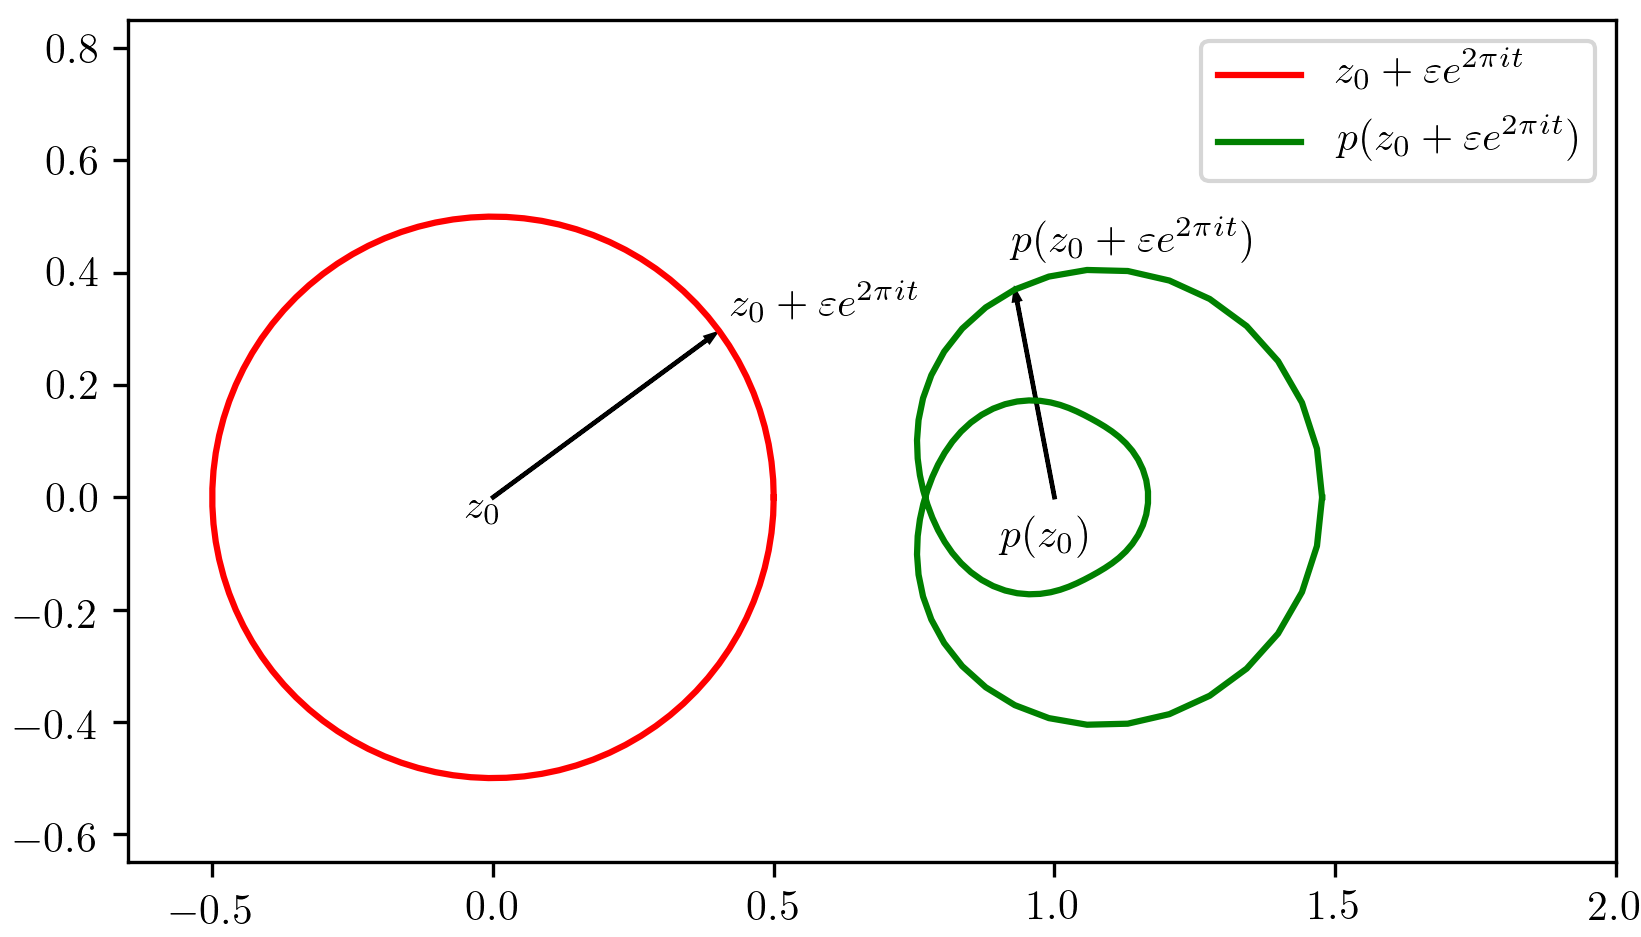
\includegraphics[scale = 0.5]{Figures/graph_cyrcle_cut.png}
\end{center}
Многочлен $p(u)$ в нуле равен нулю, а потому у него нулевой свободный член.
Тогда $p(u) = a_r u^r + \ldots + a_n u^n$, где $a_r$ -- самый младший ненулевой коэффициент ($r > 0$).
Тогда запишем $p(u) = a_r u^r (1 + \omega(u))$, где $\omega(u) = \frac{a_{r+1}}{a_r}u + \ldots + \frac{a_n}{a_r} u^{n-r}$.
Если $|u| < \varepsilon < 1$, то 
\[
|\omega(z)| \leqslant \left| \frac{a_{r+1}}{a_r}u+ \ldots + \frac{a_n}{a_r} u^{n-r}\right| \leqslant  \left|\frac{a_{r+1}}{a_r}\right| \varepsilon+ \ldots + \left|\frac{a_n}{a_r}\right| \varepsilon^{n-r} \leqslant  \left(\left|\frac{a_{r+1}}{a_r}\right|+ \ldots + \left|\frac{a_n}{a_r}\right| \right)\varepsilon
\]
Обозначим последнее выражение за $\delta(\varepsilon)$, оно стремится к нулю при $\varepsilon \to 0$.
Введем следующее обозначение $p_0(u) = a_r u^r$.
Тогда при $\varepsilon < 1$ мы можем оценить значение $p(u(t))$ на окружности $u(t) = \varepsilon e^{2\pi i t}$ следующим образом
\[
|p(u(t)) - p_0(u(t))| \leqslant |a_r| \varepsilon^r \delta(\varepsilon)
\]
Для отображения $p_0(u) = a_r u^r$ найдется $t_0$ такое, что точка $p_0(u(t_0))$ будет ближе к нулю, чем $p(z_0)$ на $ |a_r|\varepsilon^r$.
Но тогда расстояние от $p(u(t_0))$ (по неравенству треугольника) не превосходит
\[
|p(u(t_0))| \leqslant |p_0(u(t_0))| + |p(u(t_0)) - p_0(u(t_0))|  \leqslant |p(z_0)| - |a_r|\varepsilon^r + |a_r|\varepsilon^r\delta(\varepsilon) = |p(z_0)| - |a_r|\varepsilon^r(1 - \delta(\varepsilon))
\]
При малом $\varepsilon$ значение $\delta(\varepsilon)$ будет строго меньше единицы и мы получим точку $z_1 = u(t_0)$, значение в которой будет ближе к нулю, чем значение в $z_0$, что и требовалось.
\end{proof}

\subsection{Многочлены}

В этом разделе я хочу сказать пару слов про многочлены.
Пусть $F$ -- некоторое поле.
Тогда многочлен над полем $F$ -- это картинка вида $f = a_0 + a_1 x + \ldots + a_n x^n$, где $a_i\in F$.
Формально, такая картинка -- это конечная последовательность чисел $(a_0,\ldots,a_n)$, но психологически лучше и правильнее думать именно про картинки.
Еще можно для краткости писать $f = \sum_{k\geqslant 0}a_k x^k$, подразумевая, что в этой сумме только конечное число ненулевых коэффициентов.
Это удобное соображение позволяет удобно записать правила для сложения и умножения многочленов, которые определяются следующим образом
\[
\Bigl( \sum_{k\geqslant 0}a_k x^k\Bigl) + \Bigl( \sum_{k\geqslant 0}b_kx^k\Bigl) =  \sum_{k\geqslant 0}(a_k+b_k) x^k\quad\text{ и }\quad 
\Bigl( \sum_{k\geqslant 0}a_k x^k\Bigl)\Bigl( \sum_{k\geqslant 0}b_k x^k\Bigl) =  \sum_{k\geqslant 0}\Bigl(\sum_{m+n = k} a_m b_n\Bigl) x^k
\]
Таким образом многочлен -- это не функция, а картинка.
Однако, каждый многочлен $f\in F[x]$ задает функцию $F\to F$ по правилу $x\mapsto f(x)$.
Но в случае конечных полей (то есть полей из конечного числа элементов) разные многочлены могут давать одни и те же функции.
Напомню, что степень многочлена $f$ -- это наибольший номер $n$, что коэффициент $a_n\neq 0$.%
\footnote{По-хорошему надо еще аккуратно определить степень нулевого многочлена.
Но ее обычно определяют по ситуации так, как удобнее.
Например можно положить $-1$ или $-\infty$ и есть еще пара способов.
Но об этом можно особенно не запариваться.}

\paragraph{Пример}
\begin{itemize}
\item Пример конечного поля.

Пусть $p\in \mathbb Z$ -- некоторое простое число.
Обозначим через $\mathbb Z_p$ множество остатков по этому числу, то есть $\mathbb Z_p = \{0, 1, \ldots, p-1\}$.
Введем на этом множестве операции сложения и умножения по модулю простого числа $p$, то есть
\[
a + b = a + b\pmod p\quad \text{и}\quad a b = ab \pmod p
\]
Тогда можно проверить, что $Z_p$ является полем, где числа $0$ и $1$ являются нулем и единицей поля.
Единственная аксиома, которая требует усилий -- показать, что любой ненулевой элемент $Z_p$ обратим.
Давайте возьмем произвольный ненулевой элемент $a\in \mathbb Z_p$.
Так как $ a < p$ и $p$ -- простое число, то $(a, p) =1$.
По расширенному алгоритму евклида найдутся целые числа $u, v\in\mathbb Z$ такие, что $1 = u a + vp$.
Рассмотрим это равенство по модулю простого числа $p$ и получим, что
$u a = 1 \pmod p$, а это и означает, что $u$ является обратным к $a$ по умножению.

\item Пример, когда разные многочлены дают одну и ту же функцию.

Рассмотрим многочлены $\mathbb Z_2[x]$.
Тогда $\mathbb Z_2$ состоит только из $0$ и $1$.
В этом случае все многочлены $x^n$ задают одну и ту же функцию.
\end{itemize}

\begin{definition}
 Пусть $F$ -- произвольное поле и $f\in F[x]$ -- некоторый многочлен.
 Если число $a\in F$ является его корнем, то $f$ делится на $x - a$, а значит представляется в виде $f(x) = (x - a) g(x)$ для некоторого $g\in F[x]$.
 Аналогично, если $a$ является корнем $g$, то можно выделить $(x - a)$ и в $g$ и так далее.
 В итоге можно найти разложение $f(x) = (x - a)^k g(x)$, где $g(a) \neq 0$.
 В этом случае говорят, что $k$ -- это кратность корня $a$ в многочлене $f$.
 Корень кратности $1$ называется простым.
\end{definition}


\begin{definition}
Пусть $f\in F[x]$ имеет вид $f = a_0 + a_1 x + \ldots + a_n x^n$.
Определим формальную производную следующим образом $f' = a_1 + 2a_2 x+\ldots + na_n x^{n-1}$ или по-другому $f'=\sum_{k\geqslant 0} k a_k x^{k-1}$.
\end{definition}

Несложно убедиться, что, определив таким образом производную, она удовлетворяет всем естественным свойствам, к которым мы привыкли в анализе.
В качестве упражнения предлагается проверить следующее.

\begin{claim}
Пусть $F$ -- произвольное поле.
Для формальной производной выполнены следующие свойства:
\begin{enumerate}
\item $(f + g)' = f' + g'$ для любых $f,g\in F[x]$.

\item $(\lambda f )' = \lambda f'$ для любых $\lambda\in F$ и $f\in F[x]$.

\item $(fg)' = f' g + fg'$ для любых $f,g\in F[x]$.

\item $f(g(x))' = f'(g(x)) g'(x)$ для любых $f,g\in F[x]$.
\end{enumerate}
\end{claim}


С помощью формальной производной можно проверить кратность корня в произвольном многочлене.
Для начала нам нужно следующее вспомогательное утверждение.

\begin{claim}
Пусть $F$ -- произвольное поле, $f\in F[x]$ -- некоторый многочлен и $a\in F$ -- его корень кратности $k$.
Тогда 
\begin{enumerate}
\item Число $a$ является корнем кратности хотя бы $k-1$ в многочлене $f'$.

\item Если число $k 1 \neq 0$ в $F$, то $a$ является корнем кратности в точности $k - 1$ в многочлене $f'$.
\end{enumerate}
\end{claim}
\begin{proof}
1) По определению имеем $f = (x - a)^k g(x)$ причем $g(a) \neq 0$.
Возьмем производную от $f$, получим
\[
f' = k(x-a)^{k-1}g(x) + (x-a)^k g'(x) = (x-a)^{k-1}(kg(x) + (x-a)g'(x))
\]
и мы видим, что у производной $a$ имеет кратность хотя бы $k-1$.


2) Давайте поймем, когда кратность может вырасти.
Только если множитель $(kg(x) + (x-a)g'(x))$ зануляется в $a$.
Если подставить $a$, то получим $kg(a)$.
Число $g(a)\neq 0$ по выбору, но если $k 1\neq 0$, то и их произведение не ноль в поле $F$, а это будет означать, что кратность корня в точности $k - 1$.
\end{proof}

\paragraph{Примеры и замечания}
\begin{enumerate}
\item
Давайте продемонстрируем ситуацию, когда кратность корня может возрасти.
Например, выберем $F = \mathbb Z_p$ и в качестве многочлена $h$ рассмотрим $x^p - 1$.
Тогда $h' = 0$.
Теперь положим $f = xh(x) = x^{p+1}- x$.
Тогда $f' = h(x) = x^p - 1$.
С другой стороны $x^p - 1 = (x-1)^p$, а значит $1$ имеет кратность $p$ в многочлене $f$.
Но и в многочлене $f'$ $1$ имеет кратность $p$.

\item Если для любого натурального числа $k\in \mathbb N$ в поле $F$ выполнено, $k 1 \neq 0$, то можно следующим образом проверить корень многочлена $f\in F[x]$ на кратность.
Если $a\in F$ -- некоторый корень.
Надо посмотреть на $f'(a)$.
Если это число ноль, то $a$ корень кратности больше $1$, а если не ноль, то кратности в точности $1$.

\item Если $F$ произвольное поле, то общий алгоритм проверки корня на простоту следующий.
Надо взять многочлен $f\in F[x]$, для которого $a$ является корнем.
Посчитать производную $f'$, потом посчитать нод $d(x) = (f, f')$.
Если $d(a) = 0$, то $a$ кратный корень, если $d(a) \neq 0$, то это корень кратности $1$.%
\footnote{Я не буду останавливаться на доказательствах этих фактов.
Все они вам встретятся в курсе алгебры.}
\end{enumerate}



\newpage
\section{Векторные пространства}

\subsection{Идея и определение}

\paragraph{Идея}
Мы с вами до этого изучали много разных объектов, которые не сильно похожи друг на друга.
Например, вектор-столбцы $F^n$, матрицы $\operatorname{M}_{m\,n}(F)$, функции $f\colon X\to F$, многочлены $F[x]$.
Все эти товарищи нам постоянно встречаются и каждый раз приходится для каждого из них все доказывать заново и во время доказательств мы видим, что наши рассуждения повторяются.
Это означает, что на самом деле у всех этих объектов есть некий общий интерфейс, через который мы на самом деле с ним работаем.
Самое главное в этом интерфейсе то, что мы можем брать элементы из этих объектов, умножать эти элементы на числа и складывать между собой.
Абстрактное векторное пространство как раз и формализует идею такого общего интерфейса, через который в множестве можно складывать элементы и умножать на числа.


У такого подхода есть несколько плюсов.
Во-первых, формальное удобство, как только вы что-то сделали для абстрактного векторного пространства и увидели, что что-то конкретное является таковым, то все ваши достижения автоматом применимы в этой конкретной ситуации.
Общий алгоритм для векторного пространства будет одинаково хорошо работать и для столбцов, и для матриц, и для функций и т.д.
Во-вторых, есть менее очевидный бонус.
Когда мы доказываем что-то про абстрактное векторное пространство, то про него надо думать как про $F^n$.
Это поможет вам не потеряться в формализме и догадаться, что откуда берется.
Неформально это означает, что если вы что-то умеет делать для $F^n$, то это автоматически верно для любого векторного пространства!
Формально это не совсем правда, но в классе хороших пространств это так.%
\footnote{Под хорошими тут подразумеваются конечно мерные.}
Тем не менее, даже в классе всех пространств, интуиция из $F^n$ очень полезна.


\paragraph{Определение}
 Следующее определение -- это пример определения с контекстом.
Это означает, что прежде, чем его дать, вы должны зафиксировать некоторую информацию, которая необходима для вашего определения и без это информации оно -- бессмысленный мусор.
У определения векторного пространства в качестве такого контекста выступает некоторое поле $F$.
Это значит, что пока вы не зафиксировали какое-то поле, вы не можете говорить о векторных пространствах над полем $F$, а <<просто векторных пространств>> без указания какого-либо поля не существует.

\begin{definition}\label{def::VectorSpace}
Пусть $F$ -- некоторое фиксированное поле.
Тогда векторное пространство над полем $F$ -- это следующий набор данных $(V, +, \cdot)$, где
\begin{itemize}
\item $V$ -- множество.
Элементы этого множества будут называться векторами.

\item $+\colon V \times V \to V$ -- бинарная операция, то есть правило действующее так $(v,u)\mapsto v + u$, где $u,v \in V$.

\item $\cdot \colon F \times V \to V$ -- бинарная операция , то есть правило действующее так $(\alpha, v)\mapsto \alpha v$, где $\alpha \in F$ и $v\in V$.
\end{itemize}
При этом эти данные удовлетворяют следующим $8$ аксиомам:
\begin{enumerate}
\item {\bf Ассоциативность сложения} Для любых векторов $u,v,w\in V$ верно $(u+v) + w = u + (v+w)$.

\item {\bf Существование нулевого вектора} Существует такой вектор $0\in V$, что для любого $v\in V$ выполнено $0 + v = v + 0 = v$.

\item {\bf Существование противоположного вектора} Для любого вектора $v\in V$ существует вектор $-v\in V$ такой, что $v + (-v) = (-v) + v = 0$.

\item {\bf Коммутативность сложения} Для любых векторов $u,v \in V$ верно $u + v = v + u$.

\item {\bf Согласованность умножения со сложением векторов} Для любого числа $\alpha \in F$ и любых векторов $u,v \in V$ верно $\alpha(v + u) = \alpha v + \alpha u$.

\item {\bf Согласованность умножения со сложением чисел} Для любых чисел $\alpha, \beta\in F$ и любого вектора $v\in V$ верно $(\alpha + \beta)v = \alpha v + \beta v$.

\item {\bf Согласованность умножения с умножением чисел} Для любых чисел $\alpha,\beta\in F$ и любого вектора $v\in V$ верно $(\alpha\beta)v = \alpha(\beta v)$.

\item {\bf Нетривиальность} Для любого $v\in V$ верно $1 v = v$.%
\footnote{Здесь $1\in F$.}
\end{enumerate}
\end{definition}

\paragraph{Примеры}
\begin{enumerate}
\item Поле $F$ (или кто больше привык к вещественным числам $\mathbb R$) является векторным пространством над $F$ (соответственно над $\mathbb R$).

\item Более обще, множество вектор-столбцов $F^n$ является векторным пространством над $F$.

\item Множество матриц $\operatorname{M}_{m\,n}(F)$ является векторным пространством над $F$.

\item Пусть $X$ -- произвольное множество, тогда множество функций $\{f\colon X\to F\}$ является векторным пространством над $F$.
Надо лишь объяснить как складывать функции и умножать на элементы $F$.
Операции поточечные, пусть $f,g\colon X\to F$, тогда функция $(f+g)\colon X\to F$ действует по правилу $(f+g)(x) = f(x) + g(x)$.
Если $\alpha \in F$, то функция $(\alpha f)\colon X\to F$ действует по правилу $(\alpha f)(x) = \alpha f(x)$.

\item Множество многочленов $F[x] = \{a_0+a_1x + \ldots + a_n x^n\mid a_i \in F,\,n\in \mathbb Z_{\geqslant 0}\}$.
Тут надо обратить внимание, что мы подразумеваем под многочленом.
Для нас многочлен -- это НЕ функция, многочлен -- это картинка вида $a_0 + a_1 x + \ldots + a_n x^n$.%
\footnote{Для любителей формализма, можете считать, что многочлен -- это конечная последовательность элементов $F$ вида $(a_0,\ldots,a_n)$, но длина последовательности может быть любой, включая нулевую.}
Складываются и умножаются эти картинки по одинаковым правилам.
Важно, что две такие картинки равны тогда и только тогда, когда у них равные коэффициенты.
Множество всех многочленов $F[x]$ является векторным пространством над $F$.
\end{enumerate}

\paragraph{Замечание}
Стоит отметить, что в обычных векторных пространствах мы привыкли к некоторым свойствам, которые бы хотелось иметь и в общем случае.
Например, в $F^n$ есть единственный нулевой вектор, а аксиомы в общем случае говорят, что нулевой вектор лишь существует.
Однако, можно показать, что нулевой вектора автоматически единственный.
Давайте перечислим некоторые непосредственные следствия из аксиом, которые я оставляю в качестве упражнения:
\begin{enumerate}
\item Нулевой вектор единственный.

\item Для любого $v\in V$ существует единственный $-v$.

\item Для любого вектора $v\in V$ верно $-v = (-1)v$.

\item Для любого вектора $v\in V$ имеем $0 v = 0$.

\item Для любого числа $\alpha \in F$ верно $\alpha 0 = 0$.
\end{enumerate}

\subsection{Подпространство}

Пусть $V$ -- векторное пространство над $F$.
Тогда непустое подмножество $U\subseteq V$ называется подпространством, если на него можно ограничить операции $+$ и $\cdot$ и относительно них оно является векторным пространством.
Давайте определим подпространство формально.
\begin{definition}
Пусть $V$ -- векторное пространство над полем $F$.
Тогда подмножество $U\subseteq V$ называется подпространством, если
\begin{enumerate}
\item $U$ не пусто.%
\footnote{При наличии свойства~(3) это свойство эквивалентно тому, что нулевой вектор $V$ попадает в $U$.
Действительно, если он попадает, то $U$ не пусто.
Наоборот, если $u\in U$ -- какой-то вектор, то $0 = 0 u\in U$ по третьему свойству.}

\item Для любых векторов $u,u'\in U$ верно, что $u+u'\in U$.

\item Для любого скаляра $\alpha\in F$ и вектора $u\in U$ верно, что $\alpha u \in U$.
\end{enumerate}
\end{definition}
Если $U$ -- подпространство в $V$, то на $U$ можно корректно ограничить операции сложения и умножения на скаляр из исходного пространства $V$.
Таким образом у нас получается набор данных $(U, +, \cdot)$ и теперь надо, чтобы выполнялись все аксиомы векторного пространства для них.
Оказывается, что все аксиомы будут выполняться автоматически!
Например, почему у нас будет $0\in U$.
Потому что если мы возьмем любой вектор $u\in U$, то $0 = 0 u \in U$.
Остальное я оставлю в качестве упражнения.

\paragraph{Примеры}
\begin{enumerate}
\item Для любого векторного пространства $V$ подмножества $0$ и $V$ всегда являются подпространствами.

\item Множество $\{y\in F^n \mid Ay = 0\}\subseteq F^n$, где $A\in\operatorname{M}_{m\,n}(F)$, является векторным подпространством в $F^n$.
\end{enumerate}

Обратите внимание, что подпространство из второго примера кажется устроено сложнее, чем векторное пространство, в котором оно лежит $F^n$.
Однако, окажется, что взаимодействие с ними через абстрактный интерфейс векторного пространства происходит абсолютно одинаков.
То есть на самом деле подпространство устроено не сложнее, чем исходное пространство.
Об этом речь пойдет после того, как мы узнаем, что такое базисы и что значит, что какие-то векторные пространства одинаковые.

\subsection{Линейные комбинации}

\paragraph{Мотивация}
Пусть у нас есть векторное пространство $V$ над полем $F$.
Давайте поймем, а что вообще с ним можно делать?
Во-первых, $V$ -- это множество.
Значит из него можно брать элементы.
Во-вторых, там есть операция умножения на числа, то есть любой вектор можно умножить на какое-то число.
В-третьих, у нас вектора можно складывать.
Все это означает, что все что можно делать с векторным пространством, это набрать каких-то векторов из него $v_1,\ldots,v_n$ и написать выражение вида $\alpha_1 v_1 + \ldots + \alpha_n v_n$, для произвольных $\alpha_i\in F$.
Это выражение будет задавать нам какой-то вектор из $V$.
Как мы видим, особенно не разбежишься с разнообразием действий.
Однако, важно, что с помощью подобных выражений можно вытащить абсолютно всю информацию из векторных пространств, которую только возможно.
Именно поэтому все наше внимание будет посвящено выражениям такого вида, так как из них получится узнать все, что только можно про векторные пространства.

\paragraph{Линейные комбинации}

Пусть $V$ -- некоторое векторное пространство над полем $F$ и пусть $v_1,\ldots,v_n\in V$ -- некоторый набор векторов.
Тогда выражение вида $\alpha_1 v_1 +\ldots + \alpha_n v_n$, где $\alpha_i\in F$, называется линейной комбинацией $v_1,\ldots,v_n$.
Линейная комбинация называется тривиальной, если все $\alpha_i = 0$.
В противном случае она называется нетривиальной.

Вектора $v_1,\ldots,v_n\in V$ называются линейно зависимыми, если существует их нетривиальная линейная комбинация равная нулю, то есть для каких-то $\alpha_i\in F$ (так что хотя бы один не равен нулю) выражение $\alpha_1 v_1+\ldots + \alpha_n v_n = 0$.
Подчеркнем, что вектора линейно независимы, если из равенство $\alpha_1 v_1 + \ldots + \alpha_n v_n = 0$ следует, что все $\alpha_i = 0$.

\paragraph{Примеры}
\begin{enumerate}
\item Вектор $0$ всегда линейно зависим.

\item Вектор $v\in V$ линейно зависим тогда и только тогда, когда он равен нулю.

\item Вектора $v_1, v_2 \in V$ линейно зависимы тогда и только тогда, когда они пропорциональны (то есть один из них равен другому умноженному на элемент поля).
\end{enumerate}

\paragraph{Линейная оболочка}

Пусть $E\subseteq V$ -- некоторое подмножество в векторном пространстве $V$ над полем $F$.
Тогда обозначим через $\langle E \rangle$ множество всех линейных комбинаций векторов из $E$, то есть
\[
\langle E \rangle = \{\alpha_1 v_1 + \ldots + \alpha_n v_n \mid \alpha_i\in F,\, v_i \in E,\, n\in\mathbb N\}
\]
Сделаем важное замечание, если $E = \varnothing$ пусто, то $\langle \varnothing \rangle$ полагаем равным нулевому подпространству (подпространству состоящему только из нуля).
Это полезное и удобное соглашение можно понимать так: если берется линейная комбинация с нулевым числом слагаемых, то она равна нулю.

Заметим, что $\langle E \rangle$ является наименьшим векторным подпространством содержащим $E$.
Потому, для любого подпространства $U\subseteq V$ верно $\langle U \rangle  = U$.


\paragraph{Пример}

Полезно держать перед глазами следующий пример.
Пусть $V = \mathbb R^3$ -- пространство, $e_1 =(1,0,0)$, $e_2 = (0,1,0)$, $e_3 = (0,0,1)$ три вектора вдоль координатных осей.
Тогда $\langle e_1\rangle$, $\langle e_2\rangle$ и $\langle e_3\rangle$ -- это в точности координатные оси.
Подпространства $\langle e_1, e_2\rangle$, $\langle e_1, e_3\rangle$ и $\langle e_2, e_3\rangle$ -- это плоскости содержащие пары координатных осей, $\langle e_1, e_2, e_3\rangle$ будет совпадать со всем пространством $\mathbb R^3$.


		
\end{document}
